\documentclass[twoside]{book}

% Packages required by doxygen
\usepackage{calc}
\usepackage{doxygen}
\usepackage{graphicx}
\usepackage[utf8]{inputenc}
\usepackage{makeidx}
\usepackage{multicol}
\usepackage{multirow}
\usepackage{textcomp}
\usepackage[table]{xcolor}

% Font selection
\usepackage[T1]{fontenc}
\usepackage{mathptmx}
\usepackage[scaled=.90]{helvet}
\usepackage{courier}
\usepackage{amssymb}
\usepackage{sectsty}
\renewcommand{\familydefault}{\sfdefault}
\allsectionsfont{%
  \fontseries{bc}\selectfont%
  \color{darkgray}%
}
\renewcommand{\DoxyLabelFont}{%
  \fontseries{bc}\selectfont%
  \color{darkgray}%
}

% Page & text layout
\usepackage{geometry}
\geometry{%
  a4paper,%
  top=2.5cm,%
  bottom=2.5cm,%
  left=2.5cm,%
  right=2.5cm%
}
\tolerance=750
\hfuzz=15pt
\hbadness=750
\setlength{\emergencystretch}{15pt}
\setlength{\parindent}{0cm}
\setlength{\parskip}{0.2cm}
\makeatletter
\renewcommand{\paragraph}{%
  \@startsection{paragraph}{4}{0ex}{-1.0ex}{1.0ex}{%
    \normalfont\normalsize\bfseries\SS@parafont%
  }%
}
\renewcommand{\subparagraph}{%
  \@startsection{subparagraph}{5}{0ex}{-1.0ex}{1.0ex}{%
    \normalfont\normalsize\bfseries\SS@subparafont%
  }%
}
\makeatother

% Headers & footers
\usepackage{fancyhdr}
\pagestyle{fancyplain}
\fancyhead[LE]{\fancyplain{}{\bfseries\thepage}}
\fancyhead[CE]{\fancyplain{}{}}
\fancyhead[RE]{\fancyplain{}{\bfseries\leftmark}}
\fancyhead[LO]{\fancyplain{}{\bfseries\rightmark}}
\fancyhead[CO]{\fancyplain{}{}}
\fancyhead[RO]{\fancyplain{}{\bfseries\thepage}}
\fancyfoot[LE]{\fancyplain{}{}}
\fancyfoot[CE]{\fancyplain{}{}}
\fancyfoot[RE]{\fancyplain{}{\bfseries\scriptsize Generated on Wed Aug 17 2016 10\-:46\-:12 for xtdcpp \mbox{[}counters\mbox{]} by Doxygen }}
\fancyfoot[LO]{\fancyplain{}{\bfseries\scriptsize Generated on Wed Aug 17 2016 10\-:46\-:12 for xtdcpp \mbox{[}counters\mbox{]} by Doxygen }}
\fancyfoot[CO]{\fancyplain{}{}}
\fancyfoot[RO]{\fancyplain{}{}}
\renewcommand{\footrulewidth}{0.4pt}
\renewcommand{\chaptermark}[1]{%
  \markboth{#1}{}%
}
\renewcommand{\sectionmark}[1]{%
  \markright{\thesection\ #1}%
}

% Indices & bibliography
\usepackage{natbib}
\usepackage[titles]{tocloft}
\setcounter{tocdepth}{3}
\setcounter{secnumdepth}{5}
\makeindex

% Hyperlinks (required, but should be loaded last)
\usepackage{ifpdf}
\ifpdf
  \usepackage[pdftex,pagebackref=true]{hyperref}
\else
  \usepackage[ps2pdf,pagebackref=true]{hyperref}
\fi
\hypersetup{%
  colorlinks=true,%
  linkcolor=blue,%
  citecolor=blue,%
  unicode%
}

% Custom commands
\newcommand{\clearemptydoublepage}{%
  \newpage{\pagestyle{empty}\cleardoublepage}%
}


%===== C O N T E N T S =====

\begin{document}

% Titlepage & ToC
\hypersetup{pageanchor=false}
\pagenumbering{roman}
\begin{titlepage}
\vspace*{7cm}
\begin{center}%
{\Large xtdcpp \mbox{[}counters\mbox{]} }\\
\vspace*{1cm}
{\large Generated by Doxygen 1.8.6}\\
\vspace*{0.5cm}
{\small Wed Aug 17 2016 10:46:12}\\
\end{center}
\end{titlepage}
\clearemptydoublepage
\tableofcontents
\clearemptydoublepage
\pagenumbering{arabic}
\hypersetup{pageanchor=true}

%--- Begin generated contents ---
\chapter{Namespace Index}
\section{Namespace List}
Here is a list of all namespaces with brief descriptions\+:\begin{DoxyCompactList}
\item\contentsline{section}{\hyperlink{namespacextd}{xtd} }{\pageref{namespacextd}}{}
\item\contentsline{section}{\hyperlink{namespacextd_1_1servers}{xtd\+::servers} }{\pageref{namespacextd_1_1servers}}{}
\item\contentsline{section}{\hyperlink{namespacextd_1_1servers_1_1app}{xtd\+::servers\+::app} }{\pageref{namespacextd_1_1servers_1_1app}}{}
\item\contentsline{section}{\hyperlink{namespacextd_1_1servers_1_1param}{xtd\+::servers\+::param} }{\pageref{namespacextd_1_1servers_1_1param}}{}
\end{DoxyCompactList}

\chapter{Hierarchical Index}
\section{Class Hierarchy}
This inheritance list is sorted roughly, but not completely, alphabetically\-:\begin{DoxyCompactList}
\item basic\-\_\-streambuf\begin{DoxyCompactList}
\item \contentsline{section}{xtd\-:\-:network\-:\-:utils\-:\-:vectorbuf$<$ Char\-T, Traits\-T $>$}{\pageref{classxtd_1_1network_1_1utils_1_1vectorbuf}}{}
\end{DoxyCompactList}
\item \contentsline{section}{xtd\-:\-:network\-:\-:utils\-:\-:Cache\-Entry}{\pageref{structxtd_1_1network_1_1utils_1_1CacheEntry}}{}
\item \contentsline{section}{xtd\-:\-:network\-:\-:bip\-:\-:Client\-Pool$<$ T\-Request, T\-Response, T\-Domain $>$}{\pageref{classxtd_1_1network_1_1bip_1_1ClientPool}}{}
\item \contentsline{section}{xtd\-:\-:network\-:\-:utils\-:\-:Config}{\pageref{classxtd_1_1network_1_1utils_1_1Config}}{}
\item \contentsline{section}{xtd\-:\-:network\-:\-:http\-:\-:cpptempl\-:\-:Data}{\pageref{classxtd_1_1network_1_1http_1_1cpptempl_1_1Data}}{}
\begin{DoxyCompactList}
\item \contentsline{section}{xtd\-:\-:network\-:\-:http\-:\-:cpptempl\-:\-:Data\-List}{\pageref{classxtd_1_1network_1_1http_1_1cpptempl_1_1DataList}}{}
\item \contentsline{section}{xtd\-:\-:network\-:\-:http\-:\-:cpptempl\-:\-:Data\-Map}{\pageref{classxtd_1_1network_1_1http_1_1cpptempl_1_1DataMap}}{}
\item \contentsline{section}{xtd\-:\-:network\-:\-:http\-:\-:cpptempl\-:\-:Data\-Value}{\pageref{classxtd_1_1network_1_1http_1_1cpptempl_1_1DataValue}}{}
\end{DoxyCompactList}
\item \contentsline{section}{xtd\-:\-:network\-:\-:utils\-:\-:deque\-\_\-id$<$ T $>$}{\pageref{classxtd_1_1network_1_1utils_1_1deque__id}}{}
\item \contentsline{section}{xtd\-:\-:network\-:\-:utils\-:\-:deque\-\_\-id$<$ uint32\-\_\-t $>$}{\pageref{classxtd_1_1network_1_1utils_1_1deque__id}}{}
\item enable\-\_\-shared\-\_\-from\-\_\-this\begin{DoxyCompactList}
\item \contentsline{section}{xtd\-:\-:network\-:\-:base\-:\-:Connection$<$ Domain $>$}{\pageref{classxtd_1_1network_1_1base_1_1Connection}}{}
\begin{DoxyCompactList}
\item \contentsline{section}{xtd\-:\-:network\-:\-:bip\-:\-:Connection$<$ Domain $>$}{\pageref{classxtd_1_1network_1_1bip_1_1Connection}}{}
\item \contentsline{section}{xtd\-:\-:network\-:\-:http\-:\-:Connection$<$ Domain $>$}{\pageref{classxtd_1_1network_1_1http_1_1Connection}}{}
\end{DoxyCompactList}
\end{DoxyCompactList}
\item exception\begin{DoxyCompactList}
\item \contentsline{section}{xtd\-:\-:network\-:\-:http\-:\-:cpptempl\-:\-:Template\-Exception}{\pageref{classxtd_1_1network_1_1http_1_1cpptempl_1_1TemplateException}}{}
\end{DoxyCompactList}
\item function\begin{DoxyCompactList}
\item \contentsline{section}{xtd\-:\-:network\-:\-:http\-:\-:Server$<$ T\-Domain $>$\-:\-:Handler\-:\-:filter}{\pageref{structxtd_1_1network_1_1http_1_1Server_1_1Handler_1_1filter}}{}
\item \contentsline{section}{xtd\-:\-:network\-:\-:http\-:\-:Server$<$ T\-Domain $>$\-:\-:Handler\-:\-:handler}{\pageref{structxtd_1_1network_1_1http_1_1Server_1_1Handler_1_1handler}}{}
\end{DoxyCompactList}
\item \contentsline{section}{xtd\-:\-:network\-:\-:http\-:\-:Generator}{\pageref{classxtd_1_1network_1_1http_1_1Generator}}{}
\begin{DoxyCompactList}
\item \contentsline{section}{xtd\-:\-:network\-:\-:http\-:\-:Json}{\pageref{classxtd_1_1network_1_1http_1_1Json}}{}
\item \contentsline{section}{xtd\-:\-:network\-:\-:http\-:\-:Template}{\pageref{classxtd_1_1network_1_1http_1_1Template}}{}
\begin{DoxyCompactList}
\item \contentsline{section}{xtd\-:\-:network\-:\-:http\-:\-:Html\-Template}{\pageref{classxtd_1_1network_1_1http_1_1HtmlTemplate}}{}
\item \contentsline{section}{xtd\-:\-:network\-:\-:http\-:\-:Xml\-Template}{\pageref{classxtd_1_1network_1_1http_1_1XmlTemplate}}{}
\end{DoxyCompactList}
\end{DoxyCompactList}
\item \contentsline{section}{xtd\-:\-:network\-:\-:http\-:\-:Server$<$ T\-Domain $>$\-:\-:Handler}{\pageref{classxtd_1_1network_1_1http_1_1Server_1_1Handler}}{}
\item \contentsline{section}{xtd\-:\-:network\-:\-:http\-:\-:hex\-\_\-to\-\_\-string}{\pageref{structxtd_1_1network_1_1http_1_1hex__to__string}}{}
\item noncopyable\begin{DoxyCompactList}
\item \contentsline{section}{xtd\-:\-:network\-:\-:base\-:\-:Client$<$ T\-Domain $>$}{\pageref{classxtd_1_1network_1_1base_1_1Client}}{}
\begin{DoxyCompactList}
\item \contentsline{section}{xtd\-:\-:network\-:\-:bip\-:\-:Client$<$ T\-Request, T\-Response, T\-Domain $>$}{\pageref{classxtd_1_1network_1_1bip_1_1Client}}{}
\begin{DoxyCompactList}
\item \contentsline{section}{xtd\-:\-:network\-:\-:bip\-:\-:Client\-Pool$<$ T\-Request, T\-Response, T\-Domain $>$\-:\-:Persistent\-Client}{\pageref{classxtd_1_1network_1_1bip_1_1ClientPool_1_1PersistentClient}}{}
\end{DoxyCompactList}
\end{DoxyCompactList}
\item \contentsline{section}{xtd\-:\-:network\-:\-:base\-:\-:Client$<$ Domain $>$}{\pageref{classxtd_1_1network_1_1base_1_1Client}}{}
\item \contentsline{section}{xtd\-:\-:network\-:\-:base\-:\-:Connection$<$ Domain $>$}{\pageref{classxtd_1_1network_1_1base_1_1Connection}}{}
\item \contentsline{section}{xtd\-:\-:network\-:\-:base\-:\-:Server$<$ Domain $>$}{\pageref{classxtd_1_1network_1_1base_1_1Server}}{}
\begin{DoxyCompactList}
\item \contentsline{section}{xtd\-:\-:network\-:\-:bip\-:\-:Server$<$ T\-Req, T\-Res, Domain $>$}{\pageref{classxtd_1_1network_1_1bip_1_1Server}}{}
\item \contentsline{section}{xtd\-:\-:network\-:\-:http\-:\-:Server$<$ T\-Domain $>$}{\pageref{classxtd_1_1network_1_1http_1_1Server}}{}
\end{DoxyCompactList}
\item \contentsline{section}{xtd\-:\-:network\-:\-:base\-:\-:Thread\-Manager}{\pageref{classxtd_1_1network_1_1base_1_1ThreadManager}}{}
\item \contentsline{section}{xtd\-:\-:network\-:\-:utils\-:\-:Cache\-Dns}{\pageref{classxtd_1_1network_1_1utils_1_1CacheDns}}{}
\item \contentsline{section}{xtd\-:\-:network\-:\-:utils\-:\-:scoped\-\_\-method}{\pageref{classxtd_1_1network_1_1utils_1_1scoped__method}}{}
\end{DoxyCompactList}
\item \contentsline{section}{xtd\-:\-:network\-:\-:http\-:\-:Request}{\pageref{classxtd_1_1network_1_1http_1_1Request}}{}
\item \contentsline{section}{xtd\-:\-:network\-:\-:utils\-:\-:Resolver$<$ D $>$}{\pageref{classxtd_1_1network_1_1utils_1_1Resolver}}{}
\item \contentsline{section}{xtd\-:\-:network\-:\-:utils\-:\-:Resolver$<$ af\-\_\-inet $>$}{\pageref{classxtd_1_1network_1_1utils_1_1Resolver_3_01af__inet_01_4}}{}
\item \contentsline{section}{xtd\-:\-:network\-:\-:utils\-:\-:Resolver$<$ af\-\_\-unix $>$}{\pageref{classxtd_1_1network_1_1utils_1_1Resolver_3_01af__unix_01_4}}{}
\item \contentsline{section}{xtd\-:\-:network\-:\-:http\-:\-:Response}{\pageref{classxtd_1_1network_1_1http_1_1Response}}{}
\item \contentsline{section}{xtd\-:\-:network\-:\-:http\-:\-:cpptempl\-:\-:Token}{\pageref{classxtd_1_1network_1_1http_1_1cpptempl_1_1Token}}{}
\begin{DoxyCompactList}
\item \contentsline{section}{xtd\-:\-:network\-:\-:http\-:\-:cpptempl\-:\-:Token\-End}{\pageref{classxtd_1_1network_1_1http_1_1cpptempl_1_1TokenEnd}}{}
\item \contentsline{section}{xtd\-:\-:network\-:\-:http\-:\-:cpptempl\-:\-:Token\-For}{\pageref{classxtd_1_1network_1_1http_1_1cpptempl_1_1TokenFor}}{}
\item \contentsline{section}{xtd\-:\-:network\-:\-:http\-:\-:cpptempl\-:\-:Token\-If}{\pageref{classxtd_1_1network_1_1http_1_1cpptempl_1_1TokenIf}}{}
\item \contentsline{section}{xtd\-:\-:network\-:\-:http\-:\-:cpptempl\-:\-:Token\-Text}{\pageref{classxtd_1_1network_1_1http_1_1cpptempl_1_1TokenText}}{}
\item \contentsline{section}{xtd\-:\-:network\-:\-:http\-:\-:cpptempl\-:\-:Token\-Var}{\pageref{classxtd_1_1network_1_1http_1_1cpptempl_1_1TokenVar}}{}
\end{DoxyCompactList}
\end{DoxyCompactList}

\chapter{Class Index}
\section{Class List}
Here are the classes, structs, unions and interfaces with brief descriptions\+:\begin{DoxyCompactList}
\item\contentsline{section}{\hyperlink{classxtd_1_1servers_1_1app_1_1Action}{xtd\+::servers\+::app\+::\+Action} }{\pageref{classxtd_1_1servers_1_1app_1_1Action}}{}
\item\contentsline{section}{\hyperlink{structxtd_1_1servers_1_1app_1_1Address}{xtd\+::servers\+::app\+::\+Address$<$ T $>$} }{\pageref{structxtd_1_1servers_1_1app_1_1Address}}{}
\item\contentsline{section}{\hyperlink{classxtd_1_1servers_1_1param_1_1Base}{xtd\+::servers\+::param\+::\+Base} \\*Param base class }{\pageref{classxtd_1_1servers_1_1param_1_1Base}}{}
\item\contentsline{section}{\hyperlink{classxtd_1_1servers_1_1param_1_1Handler}{xtd\+::servers\+::param\+::\+Handler} \\*Param handler class }{\pageref{classxtd_1_1servers_1_1param_1_1Handler}}{}
\item\contentsline{section}{\hyperlink{classxtd_1_1servers_1_1app_1_1HtmlOArchive}{xtd\+::servers\+::app\+::\+Html\+O\+Archive} }{\pageref{classxtd_1_1servers_1_1app_1_1HtmlOArchive}}{}
\item\contentsline{section}{\hyperlink{classxtd_1_1servers_1_1app_1_1HttpServer}{xtd\+::servers\+::app\+::\+Http\+Server} }{\pageref{classxtd_1_1servers_1_1app_1_1HttpServer}}{}
\item\contentsline{section}{\hyperlink{classxtd_1_1servers_1_1param_1_1JsonVisitor}{xtd\+::servers\+::param\+::\+Json\+Visitor} \\*Json specific visitor }{\pageref{classxtd_1_1servers_1_1param_1_1JsonVisitor}}{}
\item\contentsline{section}{\hyperlink{classxtd_1_1servers_1_1param_1_1POD}{xtd\+::servers\+::param\+::\+P\+O\+D$<$ T $>$} \\*Templated param class }{\pageref{classxtd_1_1servers_1_1param_1_1POD}}{}
\item\contentsline{section}{\hyperlink{classxtd_1_1servers_1_1app_1_1Server}{xtd\+::servers\+::app\+::\+Server$<$ T\+Req, T\+Res, Domain $>$} }{\pageref{classxtd_1_1servers_1_1app_1_1Server}}{}
\item\contentsline{section}{\hyperlink{classxtd_1_1servers_1_1param_1_1Visitor}{xtd\+::servers\+::param\+::\+Visitor} \\*\hyperlink{classxtd_1_1servers_1_1param_1_1Visitor}{Visitor} base class }{\pageref{classxtd_1_1servers_1_1param_1_1Visitor}}{}
\end{DoxyCompactList}

\chapter{File Index}
\section{File List}
Here is a list of all files with brief descriptions\+:\begin{DoxyCompactList}
\item\contentsline{section}{/home/psyco/dev/xtdcpp/counters/src/\hyperlink{AvgTimedValue_8cc}{Avg\+Timed\+Value.\+cc} }{\pageref{AvgTimedValue_8cc}}{}
\item\contentsline{section}{/home/psyco/dev/xtdcpp/counters/src/\hyperlink{AvgTimedValue_8hh}{Avg\+Timed\+Value.\+hh} }{\pageref{AvgTimedValue_8hh}}{}
\item\contentsline{section}{/home/psyco/dev/xtdcpp/counters/src/\hyperlink{AvgValue_8cc}{Avg\+Value.\+cc} }{\pageref{AvgValue_8cc}}{}
\item\contentsline{section}{/home/psyco/dev/xtdcpp/counters/src/\hyperlink{AvgValue_8hh}{Avg\+Value.\+hh} }{\pageref{AvgValue_8hh}}{}
\item\contentsline{section}{/home/psyco/dev/xtdcpp/counters/src/\hyperlink{Base_8cc}{Base.\+cc} }{\pageref{Base_8cc}}{}
\item\contentsline{section}{/home/psyco/dev/xtdcpp/counters/src/\hyperlink{Base_8hh}{Base.\+hh} }{\pageref{Base_8hh}}{}
\item\contentsline{section}{/home/psyco/dev/xtdcpp/counters/src/\hyperlink{Cache_8cc}{Cache.\+cc} }{\pageref{Cache_8cc}}{}
\item\contentsline{section}{/home/psyco/dev/xtdcpp/counters/src/\hyperlink{Cache_8hh}{Cache.\+hh} }{\pageref{Cache_8hh}}{}
\item\contentsline{section}{/home/psyco/dev/xtdcpp/counters/src/\hyperlink{Composed_8cc}{Composed.\+cc} }{\pageref{Composed_8cc}}{}
\item\contentsline{section}{/home/psyco/dev/xtdcpp/counters/src/\hyperlink{Composed_8hh}{Composed.\+hh} }{\pageref{Composed_8hh}}{}
\item\contentsline{section}{/home/psyco/dev/xtdcpp/counters/src/\hyperlink{CounterManager_8cc}{Counter\+Manager.\+cc} }{\pageref{CounterManager_8cc}}{}
\item\contentsline{section}{/home/psyco/dev/xtdcpp/counters/src/\hyperlink{CounterManager_8hh}{Counter\+Manager.\+hh} }{\pageref{CounterManager_8hh}}{}
\item\contentsline{section}{/home/psyco/dev/xtdcpp/counters/src/\hyperlink{counters_8hh}{counters.\+hh} }{\pageref{counters_8hh}}{}
\item\contentsline{section}{/home/psyco/dev/xtdcpp/counters/src/\hyperlink{counters__fwd_8hh}{counters\+\_\+fwd.\+hh} }{\pageref{counters__fwd_8hh}}{}
\item\contentsline{section}{/home/psyco/dev/xtdcpp/counters/src/\hyperlink{ExtValue_8cc}{Ext\+Value.\+cc} }{\pageref{ExtValue_8cc}}{}
\item\contentsline{section}{/home/psyco/dev/xtdcpp/counters/src/\hyperlink{ExtValue_8hh}{Ext\+Value.\+hh} }{\pageref{ExtValue_8hh}}{}
\item\contentsline{section}{/home/psyco/dev/xtdcpp/counters/src/\hyperlink{FileVisitor_8hh}{File\+Visitor.\+hh} }{\pageref{FileVisitor_8hh}}{}
\item\contentsline{section}{/home/psyco/dev/xtdcpp/counters/src/\hyperlink{Freq_8cc}{Freq.\+cc} }{\pageref{Freq_8cc}}{}
\item\contentsline{section}{/home/psyco/dev/xtdcpp/counters/src/\hyperlink{Freq_8hh}{Freq.\+hh} }{\pageref{Freq_8hh}}{}
\item\contentsline{section}{/home/psyco/dev/xtdcpp/counters/src/\hyperlink{InstantFreq_8cc}{Instant\+Freq.\+cc} }{\pageref{InstantFreq_8cc}}{}
\item\contentsline{section}{/home/psyco/dev/xtdcpp/counters/src/\hyperlink{InstantFreq_8hh}{Instant\+Freq.\+hh} }{\pageref{InstantFreq_8hh}}{}
\item\contentsline{section}{/home/psyco/dev/xtdcpp/counters/src/\hyperlink{JsonVisitor_8hh}{Json\+Visitor.\+hh} }{\pageref{JsonVisitor_8hh}}{}
\item\contentsline{section}{/home/psyco/dev/xtdcpp/counters/src/\hyperlink{Perf_8cc}{Perf.\+cc} }{\pageref{Perf_8cc}}{}
\item\contentsline{section}{/home/psyco/dev/xtdcpp/counters/src/\hyperlink{Perf_8hh}{Perf.\+hh} }{\pageref{Perf_8hh}}{}
\item\contentsline{section}{/home/psyco/dev/xtdcpp/counters/src/\hyperlink{SumExt_8cc}{Sum\+Ext.\+cc} }{\pageref{SumExt_8cc}}{}
\item\contentsline{section}{/home/psyco/dev/xtdcpp/counters/src/\hyperlink{SumExt_8hh}{Sum\+Ext.\+hh} }{\pageref{SumExt_8hh}}{}
\item\contentsline{section}{/home/psyco/dev/xtdcpp/counters/src/\hyperlink{Value_8cc}{Value.\+cc} }{\pageref{Value_8cc}}{}
\item\contentsline{section}{/home/psyco/dev/xtdcpp/counters/src/\hyperlink{Value_8hh}{Value.\+hh} }{\pageref{Value_8hh}}{}
\item\contentsline{section}{/home/psyco/dev/xtdcpp/counters/src/\hyperlink{Visitor_8hh}{Visitor.\+hh} }{\pageref{Visitor_8hh}}{}
\end{DoxyCompactList}

\chapter{Namespace Documentation}
\hypertarget{namespacextd}{\section{xtd Namespace Reference}
\label{namespacextd}\index{xtd@{xtd}}
}
\subsection*{Namespaces}
\begin{DoxyCompactItemize}
\item 
\hyperlink{namespacextd_1_1text}{text}
\end{DoxyCompactItemize}
\subsection*{Classes}
\begin{DoxyCompactItemize}
\item 
class \hyperlink{classxtd_1_1Application}{Application}
\begin{DoxyCompactList}\small\item\em Parses arguments from \hyperlink{doc_2example_2Application_8hh_a6b77b2233054447db17959182b5fb02b}{main(int,char$\ast$$\ast$)} function. \end{DoxyCompactList}\item 
class \hyperlink{classxtd_1_1ConfParser}{Conf\-Parser}
\item 
class \hyperlink{classxtd_1_1error}{error}
\item 
class \hyperlink{classxtd_1_1logger}{logger}
\end{DoxyCompactItemize}
\subsection*{Enumerations}
\begin{DoxyCompactItemize}
\item 
enum \hyperlink{namespacextd_a68ed4fe8e9c11116b68efe5b102aec50}{status} \-: uint32\-\_\-t \{ \hyperlink{namespacextd_a68ed4fe8e9c11116b68efe5b102aec50a444bcb3a3fcf8389296c49467f27e1d6}{status\-::ok} = 0, 
\hyperlink{namespacextd_a68ed4fe8e9c11116b68efe5b102aec50acb5e100e5a9a3e7f6d1fd97512215282}{status\-::error} = 1, 
\hyperlink{namespacextd_a68ed4fe8e9c11116b68efe5b102aec50a90272dda245ae1fb3cf197e91a8689dc}{status\-::timeout} = 2, 
\hyperlink{namespacextd_a68ed4fe8e9c11116b68efe5b102aec50ac2adf6ecc220f2711801d6e466340183}{status\-::notfound} = 3
 \}
\end{DoxyCompactItemize}
\subsection*{Functions}
\begin{DoxyCompactItemize}
\item 
{\footnotesize template$<$typename T $>$ }\\std\-::underlying\-\_\-type$<$ T $>$\-::type \hyperlink{namespacextd_a518b0ddcbf87f6c21175d2760f4fbe21}{valueof} (T p\-\_\-item)
\end{DoxyCompactItemize}


\subsection{Enumeration Type Documentation}
\hypertarget{namespacextd_a68ed4fe8e9c11116b68efe5b102aec50}{\index{xtd@{xtd}!status@{status}}
\index{status@{status}!xtd@{xtd}}
\subsubsection[{status}]{\setlength{\rightskip}{0pt plus 5cm}enum {\bf xtd\-::status} \-: uint32\-\_\-t\hspace{0.3cm}{\ttfamily [strong]}}}\label{namespacextd_a68ed4fe8e9c11116b68efe5b102aec50}
\begin{Desc}
\item[Enumerator]\par
\begin{description}
\index{ok@{ok}!xtd@{xtd}}\index{xtd@{xtd}!ok@{ok}}\item[{\em 
\hypertarget{namespacextd_a68ed4fe8e9c11116b68efe5b102aec50a444bcb3a3fcf8389296c49467f27e1d6}{ok}\label{namespacextd_a68ed4fe8e9c11116b68efe5b102aec50a444bcb3a3fcf8389296c49467f27e1d6}
}]\index{error@{error}!xtd@{xtd}}\index{xtd@{xtd}!error@{error}}\item[{\em 
\hypertarget{namespacextd_a68ed4fe8e9c11116b68efe5b102aec50acb5e100e5a9a3e7f6d1fd97512215282}{error}\label{namespacextd_a68ed4fe8e9c11116b68efe5b102aec50acb5e100e5a9a3e7f6d1fd97512215282}
}]\index{timeout@{timeout}!xtd@{xtd}}\index{xtd@{xtd}!timeout@{timeout}}\item[{\em 
\hypertarget{namespacextd_a68ed4fe8e9c11116b68efe5b102aec50a90272dda245ae1fb3cf197e91a8689dc}{timeout}\label{namespacextd_a68ed4fe8e9c11116b68efe5b102aec50a90272dda245ae1fb3cf197e91a8689dc}
}]\index{notfound@{notfound}!xtd@{xtd}}\index{xtd@{xtd}!notfound@{notfound}}\item[{\em 
\hypertarget{namespacextd_a68ed4fe8e9c11116b68efe5b102aec50ac2adf6ecc220f2711801d6e466340183}{notfound}\label{namespacextd_a68ed4fe8e9c11116b68efe5b102aec50ac2adf6ecc220f2711801d6e466340183}
}]\end{description}
\end{Desc}


Definition at line 37 of file types.\-hh.


\begin{DoxyCode}
37 : uint32\_t \{ \hyperlink{namespacextd_a68ed4fe8e9c11116b68efe5b102aec50a444bcb3a3fcf8389296c49467f27e1d6}{ok} = 0, \hyperlink{namespacextd_a68ed4fe8e9c11116b68efe5b102aec50acb5e100e5a9a3e7f6d1fd97512215282}{error} = 1, \hyperlink{namespacextd_a68ed4fe8e9c11116b68efe5b102aec50a90272dda245ae1fb3cf197e91a8689dc}{timeout} = 2, \hyperlink{namespacextd_a68ed4fe8e9c11116b68efe5b102aec50ac2adf6ecc220f2711801d6e466340183}{notfound} = 3 \};
\end{DoxyCode}


\subsection{Function Documentation}
\hypertarget{namespacextd_a518b0ddcbf87f6c21175d2760f4fbe21}{\index{xtd@{xtd}!valueof@{valueof}}
\index{valueof@{valueof}!xtd@{xtd}}
\subsubsection[{valueof}]{\setlength{\rightskip}{0pt plus 5cm}template$<$typename T $>$ std\-::underlying\-\_\-type$<$T$>$\-::type xtd\-::valueof (
\begin{DoxyParamCaption}
\item[{T}]{p\-\_\-item}
\end{DoxyParamCaption}
)}}\label{namespacextd_a518b0ddcbf87f6c21175d2760f4fbe21}


Definition at line 32 of file types.\-hh.


\begin{DoxyCode}
33 \{
34   \textcolor{keywordflow}{return} \textcolor{keyword}{static\_cast<}typename std::underlying\_type<T>::type\textcolor{keyword}{>}(p\_item);
35 \}
\end{DoxyCode}

\hypertarget{namespacextd_1_1counters}{\section{xtd\-:\-:counters Namespace Reference}
\label{namespacextd_1_1counters}\index{xtd\-::counters@{xtd\-::counters}}
}
\subsection*{Classes}
\begin{DoxyCompactItemize}
\item 
class \hyperlink{classxtd_1_1counters_1_1AvgTimedValue}{Avg\-Timed\-Value}
\item 
class \hyperlink{classxtd_1_1counters_1_1AvgValue}{Avg\-Value}
\item 
class \hyperlink{classxtd_1_1counters_1_1Base}{Base}
\item 
class \hyperlink{classxtd_1_1counters_1_1Cache}{Cache}
\item 
class \hyperlink{classxtd_1_1counters_1_1Composed}{Composed}
\item 
class \hyperlink{classxtd_1_1counters_1_1CounterManager}{Counter\-Manager}
\item 
class \hyperlink{classxtd_1_1counters_1_1Value}{Value}
\item 
class \hyperlink{classxtd_1_1counters_1_1ExtValue}{Ext\-Value}
\item 
class \hyperlink{classxtd_1_1counters_1_1SumExt}{Sum\-Ext}
\item 
class \hyperlink{classxtd_1_1counters_1_1AvgExt}{Avg\-Ext}
\item 
class \hyperlink{classxtd_1_1counters_1_1FileVisitor}{File\-Visitor}
\item 
class \hyperlink{classxtd_1_1counters_1_1Freq}{Freq}
\item 
class \hyperlink{classxtd_1_1counters_1_1InstantFreq}{Instant\-Freq}
\item 
class \hyperlink{classxtd_1_1counters_1_1JsonVisitor}{Json\-Visitor}
\item 
class \hyperlink{classxtd_1_1counters_1_1Perf}{Perf}
\item 
class \hyperlink{classxtd_1_1counters_1_1Atomic}{Atomic}
\item 
class \hyperlink{classxtd_1_1counters_1_1Visitor}{Visitor}
\end{DoxyCompactItemize}
\subsection*{Typedefs}
\begin{DoxyCompactItemize}
\item 
typedef \hyperlink{classxtd_1_1counters_1_1AvgValue}{Avg\-Value}$<$ uint32\-\_\-t $>$ \hyperlink{namespacextd_1_1counters_a162dd5cde0e6fcc970c543f7420b4c14}{Avg\-Value32}
\item 
typedef \hyperlink{classxtd_1_1counters_1_1AvgValue}{Avg\-Value}$<$ uint64\-\_\-t $>$ \hyperlink{namespacextd_1_1counters_aa43118623f65cdf1ba43bffd8f17ea0e}{Avg\-Value64}
\item 
typedef \hyperlink{classxtd_1_1counters_1_1ExtValue}{Ext\-Value}$<$ uint32\-\_\-t $>$ \hyperlink{namespacextd_1_1counters_ae049cff0f00adb1728a511d333c2aa50}{Ext\-Value32}
\item 
typedef \hyperlink{classxtd_1_1counters_1_1ExtValue}{Ext\-Value}$<$ uint64\-\_\-t $>$ \hyperlink{namespacextd_1_1counters_ad0d26d26ad71069f92a20b6d870e4872}{Ext\-Value64}
\item 
typedef \hyperlink{classxtd_1_1counters_1_1SumExt}{Sum\-Ext}$<$ uint32\-\_\-t $>$ \hyperlink{namespacextd_1_1counters_a7e0abdd1fae0f70421c2e0ea3924db6f}{Sum\-Ext32}
\item 
typedef \hyperlink{classxtd_1_1counters_1_1SumExt}{Sum\-Ext}$<$ uint64\-\_\-t $>$ \hyperlink{namespacextd_1_1counters_a268d063d4f32d16f65c388b8791602e3}{Sum\-Ext64}
\item 
typedef \hyperlink{classxtd_1_1counters_1_1Value}{Value}$<$ uint32\-\_\-t $>$ \hyperlink{namespacextd_1_1counters_ad10dfbcb762ad7dfc7199ab5a268bc6e}{Value32}
\item 
typedef \hyperlink{classxtd_1_1counters_1_1Value}{Value}$<$ uint64\-\_\-t $>$ \hyperlink{namespacextd_1_1counters_a20cdfbbbf5aa96abb1c5d461497d1769}{Value64}
\end{DoxyCompactItemize}
\subsection*{Enumerations}
\begin{DoxyCompactItemize}
\item 
enum \hyperlink{namespacextd_1_1counters_a408a8b2fd75b44228e1741ac4a32aff8}{exec\-\_\-status} \-: uint32\-\_\-t \{ \hyperlink{namespacextd_1_1counters_a408a8b2fd75b44228e1741ac4a32aff8a1ee85f6c60017a7f0646ba8dc5824de6}{exec\-\_\-status\-::starting} = 0, 
\hyperlink{namespacextd_1_1counters_a408a8b2fd75b44228e1741ac4a32aff8a75101dcdfc88455bcafc9e53e0b06689}{exec\-\_\-status\-::running} = 1, 
\hyperlink{namespacextd_1_1counters_a408a8b2fd75b44228e1741ac4a32aff8acb5e100e5a9a3e7f6d1fd97512215282}{exec\-\_\-status\-::error} = 2, 
\hyperlink{namespacextd_1_1counters_a408a8b2fd75b44228e1741ac4a32aff8a444bcb3a3fcf8389296c49467f27e1d6}{exec\-\_\-status\-::ok} = 3
 \}
\end{DoxyCompactItemize}


\subsection{Typedef Documentation}
\hypertarget{namespacextd_1_1counters_a162dd5cde0e6fcc970c543f7420b4c14}{\index{xtd\-::counters@{xtd\-::counters}!Avg\-Value32@{Avg\-Value32}}
\index{Avg\-Value32@{Avg\-Value32}!xtd::counters@{xtd\-::counters}}
\subsubsection[{Avg\-Value32}]{\setlength{\rightskip}{0pt plus 5cm}typedef {\bf Avg\-Value}$<$uint32\-\_\-t$>$ {\bf xtd\-::counters\-::\-Avg\-Value32}}}\label{namespacextd_1_1counters_a162dd5cde0e6fcc970c543f7420b4c14}


Definition at line 50 of file Avg\-Value.\-hh.

\hypertarget{namespacextd_1_1counters_aa43118623f65cdf1ba43bffd8f17ea0e}{\index{xtd\-::counters@{xtd\-::counters}!Avg\-Value64@{Avg\-Value64}}
\index{Avg\-Value64@{Avg\-Value64}!xtd::counters@{xtd\-::counters}}
\subsubsection[{Avg\-Value64}]{\setlength{\rightskip}{0pt plus 5cm}typedef {\bf Avg\-Value}$<$uint64\-\_\-t$>$ {\bf xtd\-::counters\-::\-Avg\-Value64}}}\label{namespacextd_1_1counters_aa43118623f65cdf1ba43bffd8f17ea0e}


Definition at line 51 of file Avg\-Value.\-hh.

\hypertarget{namespacextd_1_1counters_ae049cff0f00adb1728a511d333c2aa50}{\index{xtd\-::counters@{xtd\-::counters}!Ext\-Value32@{Ext\-Value32}}
\index{Ext\-Value32@{Ext\-Value32}!xtd::counters@{xtd\-::counters}}
\subsubsection[{Ext\-Value32}]{\setlength{\rightskip}{0pt plus 5cm}typedef {\bf Ext\-Value}$<$uint32\-\_\-t$>$ {\bf xtd\-::counters\-::\-Ext\-Value32}}}\label{namespacextd_1_1counters_ae049cff0f00adb1728a511d333c2aa50}


Definition at line 28 of file Ext\-Value.\-hh.

\hypertarget{namespacextd_1_1counters_ad0d26d26ad71069f92a20b6d870e4872}{\index{xtd\-::counters@{xtd\-::counters}!Ext\-Value64@{Ext\-Value64}}
\index{Ext\-Value64@{Ext\-Value64}!xtd::counters@{xtd\-::counters}}
\subsubsection[{Ext\-Value64}]{\setlength{\rightskip}{0pt plus 5cm}typedef {\bf Ext\-Value}$<$uint64\-\_\-t$>$ {\bf xtd\-::counters\-::\-Ext\-Value64}}}\label{namespacextd_1_1counters_ad0d26d26ad71069f92a20b6d870e4872}


Definition at line 29 of file Ext\-Value.\-hh.

\hypertarget{namespacextd_1_1counters_a7e0abdd1fae0f70421c2e0ea3924db6f}{\index{xtd\-::counters@{xtd\-::counters}!Sum\-Ext32@{Sum\-Ext32}}
\index{Sum\-Ext32@{Sum\-Ext32}!xtd::counters@{xtd\-::counters}}
\subsubsection[{Sum\-Ext32}]{\setlength{\rightskip}{0pt plus 5cm}typedef {\bf Sum\-Ext}$<$uint32\-\_\-t$>$ {\bf xtd\-::counters\-::\-Sum\-Ext32}}}\label{namespacextd_1_1counters_a7e0abdd1fae0f70421c2e0ea3924db6f}


Definition at line 34 of file Sum\-Ext.\-hh.

\hypertarget{namespacextd_1_1counters_a268d063d4f32d16f65c388b8791602e3}{\index{xtd\-::counters@{xtd\-::counters}!Sum\-Ext64@{Sum\-Ext64}}
\index{Sum\-Ext64@{Sum\-Ext64}!xtd::counters@{xtd\-::counters}}
\subsubsection[{Sum\-Ext64}]{\setlength{\rightskip}{0pt plus 5cm}typedef {\bf Sum\-Ext}$<$uint64\-\_\-t$>$ {\bf xtd\-::counters\-::\-Sum\-Ext64}}}\label{namespacextd_1_1counters_a268d063d4f32d16f65c388b8791602e3}


Definition at line 35 of file Sum\-Ext.\-hh.

\hypertarget{namespacextd_1_1counters_ad10dfbcb762ad7dfc7199ab5a268bc6e}{\index{xtd\-::counters@{xtd\-::counters}!Value32@{Value32}}
\index{Value32@{Value32}!xtd::counters@{xtd\-::counters}}
\subsubsection[{Value32}]{\setlength{\rightskip}{0pt plus 5cm}typedef {\bf Value}$<$uint32\-\_\-t$>$ {\bf xtd\-::counters\-::\-Value32}}}\label{namespacextd_1_1counters_ad10dfbcb762ad7dfc7199ab5a268bc6e}


Definition at line 68 of file Value.\-hh.

\hypertarget{namespacextd_1_1counters_a20cdfbbbf5aa96abb1c5d461497d1769}{\index{xtd\-::counters@{xtd\-::counters}!Value64@{Value64}}
\index{Value64@{Value64}!xtd::counters@{xtd\-::counters}}
\subsubsection[{Value64}]{\setlength{\rightskip}{0pt plus 5cm}typedef {\bf Value}$<$uint64\-\_\-t$>$ {\bf xtd\-::counters\-::\-Value64}}}\label{namespacextd_1_1counters_a20cdfbbbf5aa96abb1c5d461497d1769}


Definition at line 69 of file Value.\-hh.



\subsection{Enumeration Type Documentation}
\hypertarget{namespacextd_1_1counters_a408a8b2fd75b44228e1741ac4a32aff8}{\index{xtd\-::counters@{xtd\-::counters}!exec\-\_\-status@{exec\-\_\-status}}
\index{exec\-\_\-status@{exec\-\_\-status}!xtd::counters@{xtd\-::counters}}
\subsubsection[{exec\-\_\-status}]{\setlength{\rightskip}{0pt plus 5cm}enum {\bf xtd\-::counters\-::exec\-\_\-status} \-: uint32\-\_\-t\hspace{0.3cm}{\ttfamily [strong]}}}\label{namespacextd_1_1counters_a408a8b2fd75b44228e1741ac4a32aff8}
\begin{Desc}
\item[Enumerator]\par
\begin{description}
\index{starting@{starting}!xtd\-::counters@{xtd\-::counters}}\index{xtd\-::counters@{xtd\-::counters}!starting@{starting}}\item[{\em 
\hypertarget{namespacextd_1_1counters_a408a8b2fd75b44228e1741ac4a32aff8a1ee85f6c60017a7f0646ba8dc5824de6}{starting}\label{namespacextd_1_1counters_a408a8b2fd75b44228e1741ac4a32aff8a1ee85f6c60017a7f0646ba8dc5824de6}
}]\index{running@{running}!xtd\-::counters@{xtd\-::counters}}\index{xtd\-::counters@{xtd\-::counters}!running@{running}}\item[{\em 
\hypertarget{namespacextd_1_1counters_a408a8b2fd75b44228e1741ac4a32aff8a75101dcdfc88455bcafc9e53e0b06689}{running}\label{namespacextd_1_1counters_a408a8b2fd75b44228e1741ac4a32aff8a75101dcdfc88455bcafc9e53e0b06689}
}]\index{error@{error}!xtd\-::counters@{xtd\-::counters}}\index{xtd\-::counters@{xtd\-::counters}!error@{error}}\item[{\em 
\hypertarget{namespacextd_1_1counters_a408a8b2fd75b44228e1741ac4a32aff8acb5e100e5a9a3e7f6d1fd97512215282}{error}\label{namespacextd_1_1counters_a408a8b2fd75b44228e1741ac4a32aff8acb5e100e5a9a3e7f6d1fd97512215282}
}]\index{ok@{ok}!xtd\-::counters@{xtd\-::counters}}\index{xtd\-::counters@{xtd\-::counters}!ok@{ok}}\item[{\em 
\hypertarget{namespacextd_1_1counters_a408a8b2fd75b44228e1741ac4a32aff8a444bcb3a3fcf8389296c49467f27e1d6}{ok}\label{namespacextd_1_1counters_a408a8b2fd75b44228e1741ac4a32aff8a444bcb3a3fcf8389296c49467f27e1d6}
}]\end{description}
\end{Desc}


Definition at line 16 of file Counter\-Manager.\-hh.


\begin{DoxyCode}
16 : uint32\_t \{ \hyperlink{namespacextd_1_1counters_a408a8b2fd75b44228e1741ac4a32aff8a1ee85f6c60017a7f0646ba8dc5824de6}{starting} = 0, \hyperlink{namespacextd_1_1counters_a408a8b2fd75b44228e1741ac4a32aff8a75101dcdfc88455bcafc9e53e0b06689}{running} = 1, \hyperlink{namespacextd_1_1counters_a408a8b2fd75b44228e1741ac4a32aff8acb5e100e5a9a3e7f6d1fd97512215282}{error} = 2, \hyperlink{namespacextd_1_1counters_a408a8b2fd75b44228e1741ac4a32aff8a444bcb3a3fcf8389296c49467f27e1d6}{ok} = 3 \};
\end{DoxyCode}

\chapter{Class Documentation}
\hypertarget{classxtd_1_1counters_1_1Atomic}{}\section{xtd\+:\+:counters\+:\+:Atomic Class Reference}
\label{classxtd_1_1counters_1_1Atomic}\index{xtd\+::counters\+::\+Atomic@{xtd\+::counters\+::\+Atomic}}


{\ttfamily \#include $<$Value.\+hh$>$}

\subsection*{Public Member Functions}
\begin{DoxyCompactItemize}
\item 
\hyperlink{classxtd_1_1counters_1_1Atomic_a54a3a8f1a29283e78a495fdd410fc3c4}{Atomic} (void)
\item 
void \hyperlink{classxtd_1_1counters_1_1Atomic_a88c5f887b5d7b70f1da87b393f12bccc}{inc} (uint32\+\_\+t \&p\+\_\+val)
\item 
void \hyperlink{classxtd_1_1counters_1_1Atomic_adb613d1d33a70c6e17d1896058a110fe}{dec} (uint32\+\_\+t \&p\+\_\+val)
\item 
void \hyperlink{classxtd_1_1counters_1_1Atomic_a90c6aa9ad58612b867df2bbdc779ca3b}{write} (uint32\+\_\+t \&p\+\_\+val, const uint32\+\_\+t \&p\+\_\+src)
\item 
{\footnotesize template$<$typename T\+Type $>$ }\\void \hyperlink{classxtd_1_1counters_1_1Atomic_adf3283f7fc1cf51af28ea2aa5822f272}{inc} (T\+Type \&p\+\_\+val)
\item 
{\footnotesize template$<$typename T\+Type $>$ }\\void \hyperlink{classxtd_1_1counters_1_1Atomic_a2bf93bdc52005c846ac43bb2afcac8f5}{dec} (T\+Type \&p\+\_\+val)
\item 
{\footnotesize template$<$typename T\+Type $>$ }\\void \hyperlink{classxtd_1_1counters_1_1Atomic_a53755a00d69b11274593f62737d9a54a}{write} (T\+Type \&p\+\_\+val, const T\+Type \&p\+\_\+src)
\end{DoxyCompactItemize}


\subsection{Detailed Description}


Definition at line 13 of file Value.\+hh.



\subsection{Constructor \& Destructor Documentation}
\index{xtd\+::counters\+::\+Atomic@{xtd\+::counters\+::\+Atomic}!Atomic@{Atomic}}
\index{Atomic@{Atomic}!xtd\+::counters\+::\+Atomic@{xtd\+::counters\+::\+Atomic}}
\subsubsection[{\texorpdfstring{Atomic(void)}{Atomic(void)}}]{\setlength{\rightskip}{0pt plus 5cm}xtd\+::counters\+::\+Atomic\+::\+Atomic (
\begin{DoxyParamCaption}
\item[{void}]{}
\end{DoxyParamCaption}
)}\hypertarget{classxtd_1_1counters_1_1Atomic_a54a3a8f1a29283e78a495fdd410fc3c4}{}\label{classxtd_1_1counters_1_1Atomic_a54a3a8f1a29283e78a495fdd410fc3c4}


Definition at line 9 of file Value.\+cc.


\begin{DoxyCode}
9                    :
10   m\_mutex()
11 \{
12 \}
\end{DoxyCode}


\subsection{Member Function Documentation}
\index{xtd\+::counters\+::\+Atomic@{xtd\+::counters\+::\+Atomic}!dec@{dec}}
\index{dec@{dec}!xtd\+::counters\+::\+Atomic@{xtd\+::counters\+::\+Atomic}}
\subsubsection[{\texorpdfstring{dec(uint32\+\_\+t \&p\+\_\+val)}{dec(uint32_t &p_val)}}]{\setlength{\rightskip}{0pt plus 5cm}void xtd\+::counters\+::\+Atomic\+::dec (
\begin{DoxyParamCaption}
\item[{uint32\+\_\+t \&}]{p\+\_\+val}
\end{DoxyParamCaption}
)}\hypertarget{classxtd_1_1counters_1_1Atomic_adb613d1d33a70c6e17d1896058a110fe}{}\label{classxtd_1_1counters_1_1Atomic_adb613d1d33a70c6e17d1896058a110fe}


Definition at line 21 of file Value.\+cc.


\begin{DoxyCode}
22 \{
23   atom::atomic\_dec32(&p\_val);
24 \}
\end{DoxyCode}
\index{xtd\+::counters\+::\+Atomic@{xtd\+::counters\+::\+Atomic}!dec@{dec}}
\index{dec@{dec}!xtd\+::counters\+::\+Atomic@{xtd\+::counters\+::\+Atomic}}
\subsubsection[{\texorpdfstring{dec(\+T\+Type \&p\+\_\+val)}{dec(TType &p_val)}}]{\setlength{\rightskip}{0pt plus 5cm}template$<$typename T\+Type $>$ void xtd\+::counters\+::\+Atomic\+::dec (
\begin{DoxyParamCaption}
\item[{T\+Type \&}]{p\+\_\+val}
\end{DoxyParamCaption}
)}\hypertarget{classxtd_1_1counters_1_1Atomic_a2bf93bdc52005c846ac43bb2afcac8f5}{}\label{classxtd_1_1counters_1_1Atomic_a2bf93bdc52005c846ac43bb2afcac8f5}
\index{xtd\+::counters\+::\+Atomic@{xtd\+::counters\+::\+Atomic}!inc@{inc}}
\index{inc@{inc}!xtd\+::counters\+::\+Atomic@{xtd\+::counters\+::\+Atomic}}
\subsubsection[{\texorpdfstring{inc(uint32\+\_\+t \&p\+\_\+val)}{inc(uint32_t &p_val)}}]{\setlength{\rightskip}{0pt plus 5cm}void xtd\+::counters\+::\+Atomic\+::inc (
\begin{DoxyParamCaption}
\item[{uint32\+\_\+t \&}]{p\+\_\+val}
\end{DoxyParamCaption}
)}\hypertarget{classxtd_1_1counters_1_1Atomic_a88c5f887b5d7b70f1da87b393f12bccc}{}\label{classxtd_1_1counters_1_1Atomic_a88c5f887b5d7b70f1da87b393f12bccc}


Definition at line 15 of file Value.\+cc.


\begin{DoxyCode}
16 \{
17   atom::atomic\_inc32(&p\_val);
18 \}
\end{DoxyCode}
\index{xtd\+::counters\+::\+Atomic@{xtd\+::counters\+::\+Atomic}!inc@{inc}}
\index{inc@{inc}!xtd\+::counters\+::\+Atomic@{xtd\+::counters\+::\+Atomic}}
\subsubsection[{\texorpdfstring{inc(\+T\+Type \&p\+\_\+val)}{inc(TType &p_val)}}]{\setlength{\rightskip}{0pt plus 5cm}template$<$typename T\+Type $>$ void xtd\+::counters\+::\+Atomic\+::inc (
\begin{DoxyParamCaption}
\item[{T\+Type \&}]{p\+\_\+val}
\end{DoxyParamCaption}
)}\hypertarget{classxtd_1_1counters_1_1Atomic_adf3283f7fc1cf51af28ea2aa5822f272}{}\label{classxtd_1_1counters_1_1Atomic_adf3283f7fc1cf51af28ea2aa5822f272}
\index{xtd\+::counters\+::\+Atomic@{xtd\+::counters\+::\+Atomic}!write@{write}}
\index{write@{write}!xtd\+::counters\+::\+Atomic@{xtd\+::counters\+::\+Atomic}}
\subsubsection[{\texorpdfstring{write(uint32\+\_\+t \&p\+\_\+val, const uint32\+\_\+t \&p\+\_\+src)}{write(uint32_t &p_val, const uint32_t &p_src)}}]{\setlength{\rightskip}{0pt plus 5cm}void xtd\+::counters\+::\+Atomic\+::write (
\begin{DoxyParamCaption}
\item[{uint32\+\_\+t \&}]{p\+\_\+val, }
\item[{const uint32\+\_\+t \&}]{p\+\_\+src}
\end{DoxyParamCaption}
)}\hypertarget{classxtd_1_1counters_1_1Atomic_a90c6aa9ad58612b867df2bbdc779ca3b}{}\label{classxtd_1_1counters_1_1Atomic_a90c6aa9ad58612b867df2bbdc779ca3b}


Definition at line 27 of file Value.\+cc.


\begin{DoxyCode}
28 \{
29   atom::atomic\_write32(&p\_val, p\_src);
30 \}
\end{DoxyCode}
\index{xtd\+::counters\+::\+Atomic@{xtd\+::counters\+::\+Atomic}!write@{write}}
\index{write@{write}!xtd\+::counters\+::\+Atomic@{xtd\+::counters\+::\+Atomic}}
\subsubsection[{\texorpdfstring{write(\+T\+Type \&p\+\_\+val, const T\+Type \&p\+\_\+src)}{write(TType &p_val, const TType &p_src)}}]{\setlength{\rightskip}{0pt plus 5cm}template$<$typename T\+Type $>$ void xtd\+::counters\+::\+Atomic\+::write (
\begin{DoxyParamCaption}
\item[{T\+Type \&}]{p\+\_\+val, }
\item[{const T\+Type \&}]{p\+\_\+src}
\end{DoxyParamCaption}
)}\hypertarget{classxtd_1_1counters_1_1Atomic_a53755a00d69b11274593f62737d9a54a}{}\label{classxtd_1_1counters_1_1Atomic_a53755a00d69b11274593f62737d9a54a}


The documentation for this class was generated from the following files\+:\begin{DoxyCompactItemize}
\item 
/home/psyco/dev/xtdcpp/counters/src/\hyperlink{Value_8hh}{Value.\+hh}\item 
/home/psyco/dev/xtdcpp/counters/src/\hyperlink{Value_8cc}{Value.\+cc}\end{DoxyCompactItemize}

\hypertarget{classxtd_1_1counters_1_1AvgExt}{}\section{xtd\+:\+:counters\+:\+:Avg\+Ext$<$ T\+Type $>$ Class Template Reference}
\label{classxtd_1_1counters_1_1AvgExt}\index{xtd\+::counters\+::\+Avg\+Ext$<$ T\+Type $>$@{xtd\+::counters\+::\+Avg\+Ext$<$ T\+Type $>$}}


{\ttfamily \#include $<$counters\+\_\+fwd.\+hh$>$}



\subsection{Detailed Description}
\subsubsection*{template$<$typename T\+Type$>$\\*
class xtd\+::counters\+::\+Avg\+Ext$<$ T\+Type $>$}



Definition at line 13 of file counters\+\_\+fwd.\+hh.



The documentation for this class was generated from the following file\+:\begin{DoxyCompactItemize}
\item 
/home/psyco/dev/xtdcpp/counters/src/\hyperlink{counters__fwd_8hh}{counters\+\_\+fwd.\+hh}\end{DoxyCompactItemize}

\hypertarget{classxtd_1_1counters_1_1AvgTimedValue}{\section{xtd\-:\-:counters\-:\-:Avg\-Timed\-Value Class Reference}
\label{classxtd_1_1counters_1_1AvgTimedValue}\index{xtd\-::counters\-::\-Avg\-Timed\-Value@{xtd\-::counters\-::\-Avg\-Timed\-Value}}
}


{\ttfamily \#include $<$Avg\-Timed\-Value.\-hh$>$}



Inheritance diagram for xtd\-:\-:counters\-:\-:Avg\-Timed\-Value\-:
\nopagebreak
\begin{figure}[H]
\begin{center}
\leavevmode
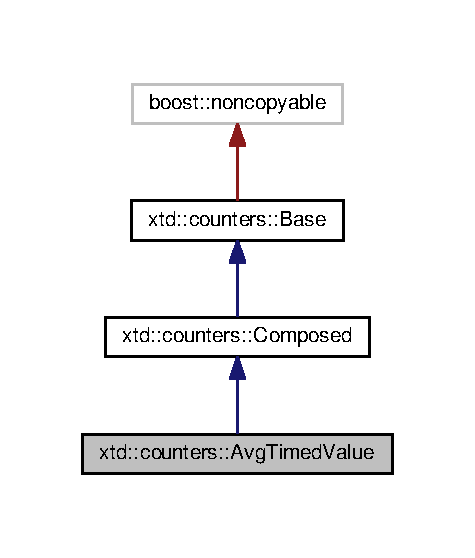
\includegraphics[width=228pt]{classxtd_1_1counters_1_1AvgTimedValue__inherit__graph}
\end{center}
\end{figure}


Collaboration diagram for xtd\-:\-:counters\-:\-:Avg\-Timed\-Value\-:
\nopagebreak
\begin{figure}[H]
\begin{center}
\leavevmode
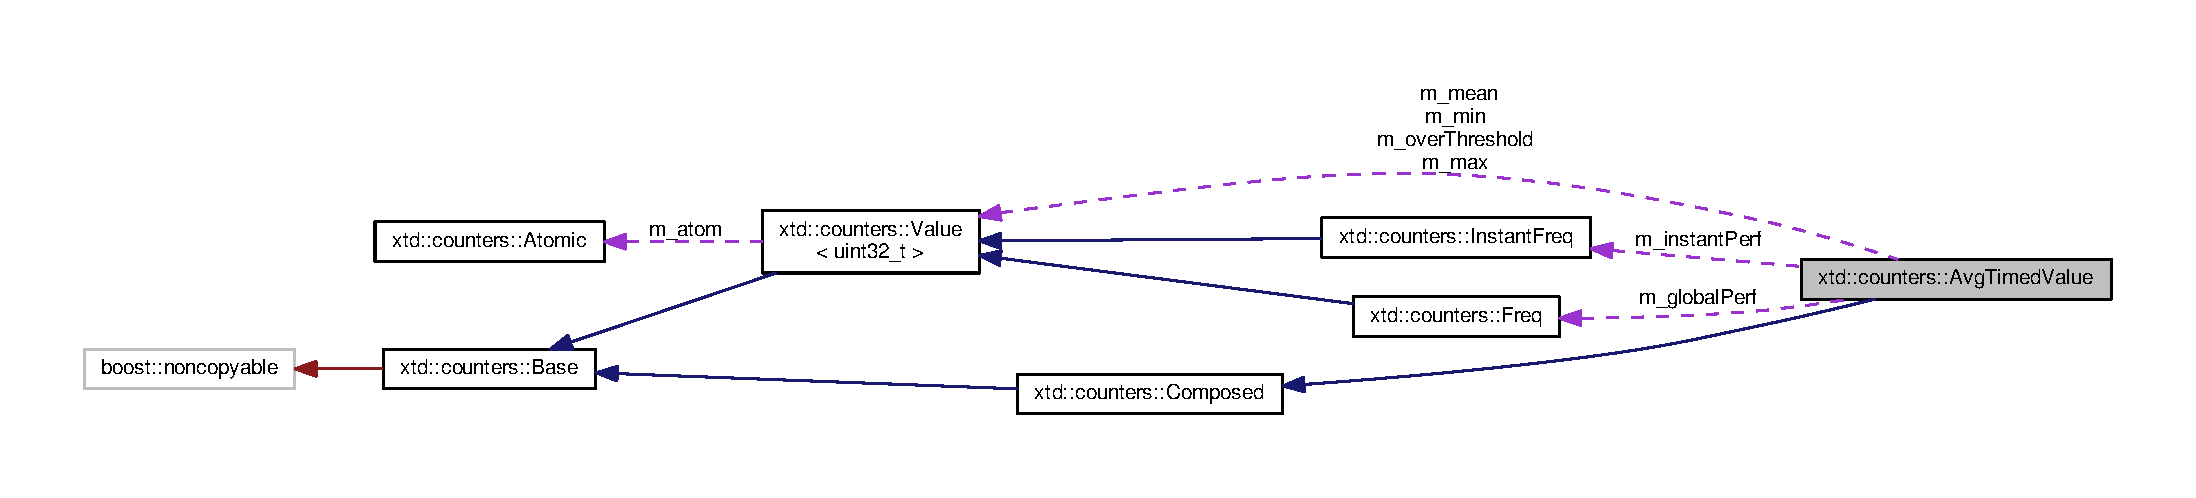
\includegraphics[width=350pt]{classxtd_1_1counters_1_1AvgTimedValue__coll__graph}
\end{center}
\end{figure}
\subsection*{Public Types}
\begin{DoxyCompactItemize}
\item 
typedef boost\-::shared\-\_\-ptr\\*
$<$ \hyperlink{classxtd_1_1counters_1_1AvgTimedValue}{Avg\-Timed\-Value} $>$ \hyperlink{classxtd_1_1counters_1_1AvgTimedValue_a68434add28044efc37c616ec7002d0f8}{t\-\_\-sptr}
\end{DoxyCompactItemize}
\subsection*{Public Member Functions}
\begin{DoxyCompactItemize}
\item 
\hyperlink{classxtd_1_1counters_1_1AvgTimedValue_a2c4e692d5e33a1155d7c869be55af0de}{Avg\-Timed\-Value} (const string \&p\-\_\-name, uint32\-\_\-t p\-\_\-nb\-Thread, uint32\-\_\-t p\-\_\-time\-Delta\-Ms=5 $\ast$60 $\ast$1000, uint32\-\_\-t p\-\_\-threshold\-Ms=0)
\item 
virtual \hyperlink{classxtd_1_1counters_1_1AvgTimedValue_a08aa140f45a1160943a494e5eab59aa7}{$\sim$\-Avg\-Timed\-Value} (void)
\item 
void \hyperlink{classxtd_1_1counters_1_1AvgTimedValue_ab5b5b6e1b4dae4bb4172ebc11ffc7c91}{start\-Chrono} (uint32\-\_\-t p\-\_\-request\-I\-D)
\item 
void \hyperlink{classxtd_1_1counters_1_1AvgTimedValue_a9a6818ff8c4f882a1445e9c49ed79e0f}{stop\-Chrono} (uint32\-\_\-t p\-\_\-request\-I\-D)
\item 
void \hyperlink{classxtd_1_1counters_1_1AvgTimedValue_a8d3f9dbf787c7c307957038a879fb69a}{add\-Response\-Time} (uint32\-\_\-t p\-\_\-time\-Us)
\item 
void \hyperlink{classxtd_1_1counters_1_1AvgTimedValue_a789b1bdb5596f6cb332435892411dbb0}{set\-Assert} (const bool p\-\_\-assert)
\end{DoxyCompactItemize}
\subsection*{Public Attributes}
\begin{DoxyCompactItemize}
\item 
\hyperlink{classxtd_1_1counters_1_1AvgTimedValue_a71d5e67cb282762c880dc4986e5a8d7c}{t\-\_\-samples} \hyperlink{classxtd_1_1counters_1_1AvgTimedValue_af33c7f1f69e37ef49e4195de8f4ac6e2}{m\-\_\-samples}
\item 
\hyperlink{classxtd_1_1counters_1_1AvgTimedValue_a901afa3b937939c2132a593d4a801cad}{t\-\_\-timevect} \hyperlink{classxtd_1_1counters_1_1AvgTimedValue_aff4e550c326e9e16ad2f9e5ff384ae2e}{m\-\_\-start\-Times}
\item 
vector$<$ uint32\-\_\-t $>$ \hyperlink{classxtd_1_1counters_1_1AvgTimedValue_a9f3477cd3eb3fb75f2ba8d75d706eb88}{m\-\_\-reseted}
\item 
\hyperlink{classxtd_1_1counters_1_1Freq}{Freq} \hyperlink{classxtd_1_1counters_1_1AvgTimedValue_ad0b3148989210f269416e5af2169278e}{m\-\_\-global\-Perf}
\item 
\hyperlink{classxtd_1_1counters_1_1InstantFreq}{Instant\-Freq} \hyperlink{classxtd_1_1counters_1_1AvgTimedValue_a16f6336d72850b29aa10a97d72309ec4}{m\-\_\-instant\-Perf}
\item 
\hyperlink{namespacextd_1_1counters_ad10dfbcb762ad7dfc7199ab5a268bc6e}{Value32} \hyperlink{classxtd_1_1counters_1_1AvgTimedValue_ab0eb52c60a1fe28c6ea148270ca8cc74}{m\-\_\-mean}
\item 
\hyperlink{namespacextd_1_1counters_ad10dfbcb762ad7dfc7199ab5a268bc6e}{Value32} \hyperlink{classxtd_1_1counters_1_1AvgTimedValue_aeed066e7062c73d577033308bc0344bf}{m\-\_\-min}
\item 
\hyperlink{namespacextd_1_1counters_ad10dfbcb762ad7dfc7199ab5a268bc6e}{Value32} \hyperlink{classxtd_1_1counters_1_1AvgTimedValue_a90ef2640c6d711a3eef2585aaef50afb}{m\-\_\-max}
\item 
\hyperlink{namespacextd_1_1counters_ad10dfbcb762ad7dfc7199ab5a268bc6e}{Value32} \hyperlink{classxtd_1_1counters_1_1AvgTimedValue_a7a91ad83dade8f67c4df8150ddb33060}{m\-\_\-over\-Threshold}
\item 
const uint32\-\_\-t \hyperlink{classxtd_1_1counters_1_1AvgTimedValue_a2986c9cf3526f6f86d340dafd25ae04f}{m\-\_\-time\-Delta\-Ms}
\item 
const uint32\-\_\-t \hyperlink{classxtd_1_1counters_1_1AvgTimedValue_a96ae1248a1019b22cf41bae4a47314c2}{m\-\_\-threshold\-Ms}
\item 
bool \hyperlink{classxtd_1_1counters_1_1AvgTimedValue_a6e4edcfa3fcd639b23195119f2b28bd3}{m\-\_\-assert}
\end{DoxyCompactItemize}
\subsection*{Protected Types}
\begin{DoxyCompactItemize}
\item 
typedef std\-::pair\\*
$<$ boost\-::posix\-\_\-time\-::ptime, \\*
uint32\-\_\-t $>$ \hyperlink{classxtd_1_1counters_1_1AvgTimedValue_a1495aff37899fa6b011aed1b4283db18}{t\-\_\-elem}
\item 
typedef std\-::deque$<$ \hyperlink{classxtd_1_1counters_1_1AvgTimedValue_a1495aff37899fa6b011aed1b4283db18}{t\-\_\-elem} $>$ \hyperlink{classxtd_1_1counters_1_1AvgTimedValue_a71d5e67cb282762c880dc4986e5a8d7c}{t\-\_\-samples}
\item 
typedef std\-::deque\\*
$<$ boost\-::posix\-\_\-time\-::ptime $>$ \hyperlink{classxtd_1_1counters_1_1AvgTimedValue_a901afa3b937939c2132a593d4a801cad}{t\-\_\-timevect}
\end{DoxyCompactItemize}
\subsection*{Protected Member Functions}
\begin{DoxyCompactItemize}
\item 
void \hyperlink{classxtd_1_1counters_1_1AvgTimedValue_a1430fd5ff91e960a251b0656c2b5c0ca}{update\-\_\-safe} (void)
\end{DoxyCompactItemize}
\subsection*{Friends}
\begin{DoxyCompactItemize}
\item 
class \hyperlink{classxtd_1_1counters_1_1AvgTimedValue_a93e934ad70d5b32b14beed5572450abf}{Composed}
\end{DoxyCompactItemize}
\subsection*{Additional Inherited Members}


\subsection{Detailed Description}


Definition at line 19 of file Avg\-Timed\-Value.\-hh.



\subsection{Member Typedef Documentation}
\hypertarget{classxtd_1_1counters_1_1AvgTimedValue_a1495aff37899fa6b011aed1b4283db18}{\index{xtd\-::counters\-::\-Avg\-Timed\-Value@{xtd\-::counters\-::\-Avg\-Timed\-Value}!t\-\_\-elem@{t\-\_\-elem}}
\index{t\-\_\-elem@{t\-\_\-elem}!xtd::counters::AvgTimedValue@{xtd\-::counters\-::\-Avg\-Timed\-Value}}
\subsubsection[{t\-\_\-elem}]{\setlength{\rightskip}{0pt plus 5cm}typedef std\-::pair$<$boost\-::posix\-\_\-time\-::ptime, uint32\-\_\-t$>$ {\bf xtd\-::counters\-::\-Avg\-Timed\-Value\-::t\-\_\-elem}\hspace{0.3cm}{\ttfamily [protected]}}}\label{classxtd_1_1counters_1_1AvgTimedValue_a1495aff37899fa6b011aed1b4283db18}


Definition at line 24 of file Avg\-Timed\-Value.\-hh.

\hypertarget{classxtd_1_1counters_1_1AvgTimedValue_a71d5e67cb282762c880dc4986e5a8d7c}{\index{xtd\-::counters\-::\-Avg\-Timed\-Value@{xtd\-::counters\-::\-Avg\-Timed\-Value}!t\-\_\-samples@{t\-\_\-samples}}
\index{t\-\_\-samples@{t\-\_\-samples}!xtd::counters::AvgTimedValue@{xtd\-::counters\-::\-Avg\-Timed\-Value}}
\subsubsection[{t\-\_\-samples}]{\setlength{\rightskip}{0pt plus 5cm}typedef std\-::deque$<${\bf t\-\_\-elem}$>$ {\bf xtd\-::counters\-::\-Avg\-Timed\-Value\-::t\-\_\-samples}\hspace{0.3cm}{\ttfamily [protected]}}}\label{classxtd_1_1counters_1_1AvgTimedValue_a71d5e67cb282762c880dc4986e5a8d7c}


Definition at line 25 of file Avg\-Timed\-Value.\-hh.

\hypertarget{classxtd_1_1counters_1_1AvgTimedValue_a68434add28044efc37c616ec7002d0f8}{\index{xtd\-::counters\-::\-Avg\-Timed\-Value@{xtd\-::counters\-::\-Avg\-Timed\-Value}!t\-\_\-sptr@{t\-\_\-sptr}}
\index{t\-\_\-sptr@{t\-\_\-sptr}!xtd::counters::AvgTimedValue@{xtd\-::counters\-::\-Avg\-Timed\-Value}}
\subsubsection[{t\-\_\-sptr}]{\setlength{\rightskip}{0pt plus 5cm}typedef boost\-::shared\-\_\-ptr$<${\bf Avg\-Timed\-Value}$>$ {\bf xtd\-::counters\-::\-Avg\-Timed\-Value\-::t\-\_\-sptr}}}\label{classxtd_1_1counters_1_1AvgTimedValue_a68434add28044efc37c616ec7002d0f8}


Definition at line 29 of file Avg\-Timed\-Value.\-hh.

\hypertarget{classxtd_1_1counters_1_1AvgTimedValue_a901afa3b937939c2132a593d4a801cad}{\index{xtd\-::counters\-::\-Avg\-Timed\-Value@{xtd\-::counters\-::\-Avg\-Timed\-Value}!t\-\_\-timevect@{t\-\_\-timevect}}
\index{t\-\_\-timevect@{t\-\_\-timevect}!xtd::counters::AvgTimedValue@{xtd\-::counters\-::\-Avg\-Timed\-Value}}
\subsubsection[{t\-\_\-timevect}]{\setlength{\rightskip}{0pt plus 5cm}typedef std\-::deque$<$ boost\-::posix\-\_\-time\-::ptime $>$ {\bf xtd\-::counters\-::\-Avg\-Timed\-Value\-::t\-\_\-timevect}\hspace{0.3cm}{\ttfamily [protected]}}}\label{classxtd_1_1counters_1_1AvgTimedValue_a901afa3b937939c2132a593d4a801cad}


Definition at line 26 of file Avg\-Timed\-Value.\-hh.



\subsection{Constructor \& Destructor Documentation}
\hypertarget{classxtd_1_1counters_1_1AvgTimedValue_a2c4e692d5e33a1155d7c869be55af0de}{\index{xtd\-::counters\-::\-Avg\-Timed\-Value@{xtd\-::counters\-::\-Avg\-Timed\-Value}!Avg\-Timed\-Value@{Avg\-Timed\-Value}}
\index{Avg\-Timed\-Value@{Avg\-Timed\-Value}!xtd::counters::AvgTimedValue@{xtd\-::counters\-::\-Avg\-Timed\-Value}}
\subsubsection[{Avg\-Timed\-Value}]{\setlength{\rightskip}{0pt plus 5cm}xtd\-::counters\-::\-Avg\-Timed\-Value\-::\-Avg\-Timed\-Value (
\begin{DoxyParamCaption}
\item[{const string \&}]{p\-\_\-name, }
\item[{uint32\-\_\-t}]{p\-\_\-nb\-Thread, }
\item[{uint32\-\_\-t}]{p\-\_\-time\-Delta\-Ms = {\ttfamily 5~$\ast$~60~$\ast$~1000}, }
\item[{uint32\-\_\-t}]{p\-\_\-threshold\-Ms = {\ttfamily 0}}
\end{DoxyParamCaption}
)}}\label{classxtd_1_1counters_1_1AvgTimedValue_a2c4e692d5e33a1155d7c869be55af0de}


Definition at line 16 of file Avg\-Timed\-Value.\-cc.


\begin{DoxyCode}
19                                                      :
20   \hyperlink{classxtd_1_1counters_1_1AvgTimedValue_a93e934ad70d5b32b14beed5572450abf}{Composed}(p\_name),
21   \hyperlink{classxtd_1_1counters_1_1AvgTimedValue_af33c7f1f69e37ef49e4195de8f4ac6e2}{m\_samples}(),
22   \hyperlink{classxtd_1_1counters_1_1AvgTimedValue_aff4e550c326e9e16ad2f9e5ff384ae2e}{m\_startTimes}(p\_nbThread),
23   \hyperlink{classxtd_1_1counters_1_1AvgTimedValue_a9f3477cd3eb3fb75f2ba8d75d706eb88}{m\_reseted}(p\_nbThread, 0),
24   \hyperlink{classxtd_1_1counters_1_1AvgTimedValue_ad0b3148989210f269416e5af2169278e}{m\_globalPerf}(\textcolor{stringliteral}{"perf"}),
25   \hyperlink{classxtd_1_1counters_1_1AvgTimedValue_a16f6336d72850b29aa10a97d72309ec4}{m\_instantPerf}(\textcolor{stringliteral}{"instant.perf"}),
26   \hyperlink{classxtd_1_1counters_1_1AvgTimedValue_ab0eb52c60a1fe28c6ea148270ca8cc74}{m\_mean}(\textcolor{stringliteral}{"RTT.moy"}),
27   \hyperlink{classxtd_1_1counters_1_1AvgTimedValue_aeed066e7062c73d577033308bc0344bf}{m\_min}(\textcolor{stringliteral}{"RTT.min"}),
28   \hyperlink{classxtd_1_1counters_1_1AvgTimedValue_a90ef2640c6d711a3eef2585aaef50afb}{m\_max}(\textcolor{stringliteral}{"RTT.max"}),
29   \hyperlink{classxtd_1_1counters_1_1AvgTimedValue_a7a91ad83dade8f67c4df8150ddb33060}{m\_overThreshold}(\textcolor{stringliteral}{"RTT.threshold"}),
30   \hyperlink{classxtd_1_1counters_1_1AvgTimedValue_a2986c9cf3526f6f86d340dafd25ae04f}{m\_timeDeltaMs}(p\_timeDeltaMs),
31   \hyperlink{classxtd_1_1counters_1_1AvgTimedValue_a96ae1248a1019b22cf41bae4a47314c2}{m\_thresholdMs}(p\_thresholdMs),
32   \hyperlink{classxtd_1_1counters_1_1AvgTimedValue_a6e4edcfa3fcd639b23195119f2b28bd3}{m\_assert}(\textcolor{keyword}{false})
33 \{
34   \hyperlink{classxtd_1_1counters_1_1Composed_ac2efbce59510b352a2d47b3118e0d02a}{addItem}(\hyperlink{classxtd_1_1counters_1_1AvgTimedValue_ad0b3148989210f269416e5af2169278e}{m\_globalPerf});
35   \hyperlink{classxtd_1_1counters_1_1Composed_ac2efbce59510b352a2d47b3118e0d02a}{addItem}(\hyperlink{classxtd_1_1counters_1_1AvgTimedValue_a16f6336d72850b29aa10a97d72309ec4}{m\_instantPerf});
36   \hyperlink{classxtd_1_1counters_1_1Composed_ac2efbce59510b352a2d47b3118e0d02a}{addItem}(\hyperlink{classxtd_1_1counters_1_1AvgTimedValue_ab0eb52c60a1fe28c6ea148270ca8cc74}{m\_mean});
37   \hyperlink{classxtd_1_1counters_1_1Composed_ac2efbce59510b352a2d47b3118e0d02a}{addItem}(\hyperlink{classxtd_1_1counters_1_1AvgTimedValue_aeed066e7062c73d577033308bc0344bf}{m\_min});
38   \hyperlink{classxtd_1_1counters_1_1Composed_ac2efbce59510b352a2d47b3118e0d02a}{addItem}(\hyperlink{classxtd_1_1counters_1_1AvgTimedValue_a90ef2640c6d711a3eef2585aaef50afb}{m\_max});
39   \hyperlink{classxtd_1_1counters_1_1Composed_ac2efbce59510b352a2d47b3118e0d02a}{addItem}(\hyperlink{classxtd_1_1counters_1_1AvgTimedValue_a7a91ad83dade8f67c4df8150ddb33060}{m\_overThreshold});
40 
41   \hyperlink{classxtd_1_1counters_1_1AvgTimedValue_ab0eb52c60a1fe28c6ea148270ca8cc74}{m\_mean}.\hyperlink{classxtd_1_1counters_1_1Value_ab206db077ef38ac776a7e64774f56f2b}{NaN}();
42   \hyperlink{classxtd_1_1counters_1_1AvgTimedValue_aeed066e7062c73d577033308bc0344bf}{m\_min}.\hyperlink{classxtd_1_1counters_1_1Value_ab206db077ef38ac776a7e64774f56f2b}{NaN}();
43   \hyperlink{classxtd_1_1counters_1_1AvgTimedValue_a90ef2640c6d711a3eef2585aaef50afb}{m\_max}.\hyperlink{classxtd_1_1counters_1_1Value_ab206db077ef38ac776a7e64774f56f2b}{NaN}();
44   \hyperlink{classxtd_1_1counters_1_1AvgTimedValue_a7a91ad83dade8f67c4df8150ddb33060}{m\_overThreshold} = 0;
45   \hyperlink{classxtd_1_1counters_1_1AvgTimedValue_ad0b3148989210f269416e5af2169278e}{m\_globalPerf}    = 0;
46   \hyperlink{classxtd_1_1counters_1_1AvgTimedValue_a16f6336d72850b29aa10a97d72309ec4}{m\_instantPerf}   = 0;
47 \}
\end{DoxyCode}


Here is the call graph for this function\-:
\nopagebreak
\begin{figure}[H]
\begin{center}
\leavevmode
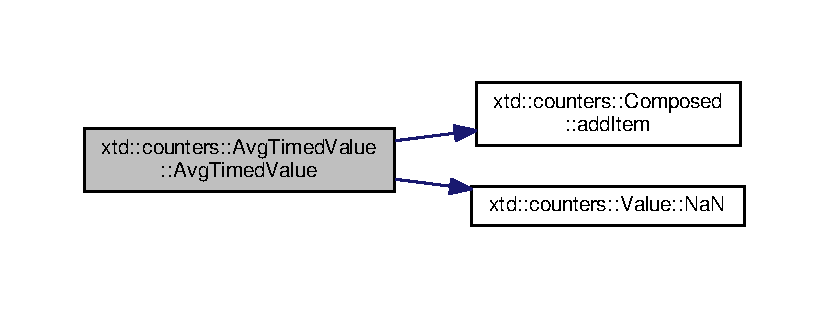
\includegraphics[width=350pt]{classxtd_1_1counters_1_1AvgTimedValue_a2c4e692d5e33a1155d7c869be55af0de_cgraph}
\end{center}
\end{figure}


\hypertarget{classxtd_1_1counters_1_1AvgTimedValue_a08aa140f45a1160943a494e5eab59aa7}{\index{xtd\-::counters\-::\-Avg\-Timed\-Value@{xtd\-::counters\-::\-Avg\-Timed\-Value}!$\sim$\-Avg\-Timed\-Value@{$\sim$\-Avg\-Timed\-Value}}
\index{$\sim$\-Avg\-Timed\-Value@{$\sim$\-Avg\-Timed\-Value}!xtd::counters::AvgTimedValue@{xtd\-::counters\-::\-Avg\-Timed\-Value}}
\subsubsection[{$\sim$\-Avg\-Timed\-Value}]{\setlength{\rightskip}{0pt plus 5cm}virtual xtd\-::counters\-::\-Avg\-Timed\-Value\-::$\sim$\-Avg\-Timed\-Value (
\begin{DoxyParamCaption}
\item[{void}]{}
\end{DoxyParamCaption}
)\hspace{0.3cm}{\ttfamily [inline]}, {\ttfamily [virtual]}}}\label{classxtd_1_1counters_1_1AvgTimedValue_a08aa140f45a1160943a494e5eab59aa7}


Definition at line 37 of file Avg\-Timed\-Value.\-hh.


\begin{DoxyCode}
37 \{\};
\end{DoxyCode}


\subsection{Member Function Documentation}
\hypertarget{classxtd_1_1counters_1_1AvgTimedValue_a8d3f9dbf787c7c307957038a879fb69a}{\index{xtd\-::counters\-::\-Avg\-Timed\-Value@{xtd\-::counters\-::\-Avg\-Timed\-Value}!add\-Response\-Time@{add\-Response\-Time}}
\index{add\-Response\-Time@{add\-Response\-Time}!xtd::counters::AvgTimedValue@{xtd\-::counters\-::\-Avg\-Timed\-Value}}
\subsubsection[{add\-Response\-Time}]{\setlength{\rightskip}{0pt plus 5cm}void xtd\-::counters\-::\-Avg\-Timed\-Value\-::add\-Response\-Time (
\begin{DoxyParamCaption}
\item[{uint32\-\_\-t}]{p\-\_\-time\-Us}
\end{DoxyParamCaption}
)}}\label{classxtd_1_1counters_1_1AvgTimedValue_a8d3f9dbf787c7c307957038a879fb69a}


Definition at line 84 of file Avg\-Timed\-Value.\-cc.


\begin{DoxyCode}
85 \{
86   boost::mutex::scoped\_lock l\_lock(\hyperlink{classxtd_1_1counters_1_1Base_aeeac2ffcae02eb6341418d708188a353}{m\_mutex});
87   responsetime\_safe(p\_timeUs);
88 \}
\end{DoxyCode}
\hypertarget{classxtd_1_1counters_1_1AvgTimedValue_a789b1bdb5596f6cb332435892411dbb0}{\index{xtd\-::counters\-::\-Avg\-Timed\-Value@{xtd\-::counters\-::\-Avg\-Timed\-Value}!set\-Assert@{set\-Assert}}
\index{set\-Assert@{set\-Assert}!xtd::counters::AvgTimedValue@{xtd\-::counters\-::\-Avg\-Timed\-Value}}
\subsubsection[{set\-Assert}]{\setlength{\rightskip}{0pt plus 5cm}void xtd\-::counters\-::\-Avg\-Timed\-Value\-::set\-Assert (
\begin{DoxyParamCaption}
\item[{const bool}]{p\-\_\-assert}
\end{DoxyParamCaption}
)}}\label{classxtd_1_1counters_1_1AvgTimedValue_a789b1bdb5596f6cb332435892411dbb0}


Definition at line 197 of file Avg\-Timed\-Value.\-cc.


\begin{DoxyCode}
198 \{
199   \hyperlink{classxtd_1_1counters_1_1AvgTimedValue_a6e4edcfa3fcd639b23195119f2b28bd3}{m\_assert} = p\_assert;
200 \}
\end{DoxyCode}
\hypertarget{classxtd_1_1counters_1_1AvgTimedValue_ab5b5b6e1b4dae4bb4172ebc11ffc7c91}{\index{xtd\-::counters\-::\-Avg\-Timed\-Value@{xtd\-::counters\-::\-Avg\-Timed\-Value}!start\-Chrono@{start\-Chrono}}
\index{start\-Chrono@{start\-Chrono}!xtd::counters::AvgTimedValue@{xtd\-::counters\-::\-Avg\-Timed\-Value}}
\subsubsection[{start\-Chrono}]{\setlength{\rightskip}{0pt plus 5cm}void xtd\-::counters\-::\-Avg\-Timed\-Value\-::start\-Chrono (
\begin{DoxyParamCaption}
\item[{uint32\-\_\-t}]{p\-\_\-request\-I\-D}
\end{DoxyParamCaption}
)}}\label{classxtd_1_1counters_1_1AvgTimedValue_ab5b5b6e1b4dae4bb4172ebc11ffc7c91}


Definition at line 50 of file Avg\-Timed\-Value.\-cc.


\begin{DoxyCode}
51 \{
52   \textcolor{keywordflow}{if}(\hyperlink{classxtd_1_1counters_1_1AvgTimedValue_a9f3477cd3eb3fb75f2ba8d75d706eb88}{m\_reseted}[p\_requestID] == 1)
53   \{
54     logger::crit(\textcolor{stringliteral}{"counters.avgtimedvalue"}, \textcolor{stringliteral}{"AvgTimedValue chrono started but not stopped (ID:%d)!!! Cancel
       init start date. "}, p\_requestID, HERE);
55   \}
56   \textcolor{keywordflow}{else}
57   \{
58     \hyperlink{classxtd_1_1counters_1_1AvgTimedValue_aff4e550c326e9e16ad2f9e5ff384ae2e}{m\_startTimes}[p\_requestID] = bpt::microsec\_clock::local\_time();
59   \}
60 
61   \hyperlink{classxtd_1_1counters_1_1AvgTimedValue_a9f3477cd3eb3fb75f2ba8d75d706eb88}{m\_reseted}[p\_requestID] = 1;
62 \}
\end{DoxyCode}
\hypertarget{classxtd_1_1counters_1_1AvgTimedValue_a9a6818ff8c4f882a1445e9c49ed79e0f}{\index{xtd\-::counters\-::\-Avg\-Timed\-Value@{xtd\-::counters\-::\-Avg\-Timed\-Value}!stop\-Chrono@{stop\-Chrono}}
\index{stop\-Chrono@{stop\-Chrono}!xtd::counters::AvgTimedValue@{xtd\-::counters\-::\-Avg\-Timed\-Value}}
\subsubsection[{stop\-Chrono}]{\setlength{\rightskip}{0pt plus 5cm}void xtd\-::counters\-::\-Avg\-Timed\-Value\-::stop\-Chrono (
\begin{DoxyParamCaption}
\item[{uint32\-\_\-t}]{p\-\_\-request\-I\-D}
\end{DoxyParamCaption}
)}}\label{classxtd_1_1counters_1_1AvgTimedValue_a9a6818ff8c4f882a1445e9c49ed79e0f}


Definition at line 65 of file Avg\-Timed\-Value.\-cc.


\begin{DoxyCode}
66 \{
67   boost::mutex::scoped\_lock l\_lock(\hyperlink{classxtd_1_1counters_1_1Base_aeeac2ffcae02eb6341418d708188a353}{m\_mutex});
68 
69   \textcolor{keywordflow}{if} (\hyperlink{classxtd_1_1counters_1_1AvgTimedValue_a9f3477cd3eb3fb75f2ba8d75d706eb88}{m\_reseted}[p\_requestID] == 0)
70   \{
71     logger::crit(\textcolor{stringliteral}{"counters.avgtimedvalue"}, \textcolor{stringliteral}{"AvgTimedValue chrono stopped but not started (ID:%d)!!! Value
       is discarded. "}, p\_requestID, HERE);
72     \textcolor{keywordflow}{return};
73   \}
74 
75   bpt::ptime         l\_now      = bpt::microsec\_clock::local\_time();
76   bpt::time\_duration l\_diffTime = l\_now - \hyperlink{classxtd_1_1counters_1_1AvgTimedValue_aff4e550c326e9e16ad2f9e5ff384ae2e}{m\_startTimes}[p\_requestID];
77   uint32\_t           l\_timeUs   = l\_diffTime.total\_microseconds();
78 
79   responsetime\_safe(l\_timeUs);
80   \hyperlink{classxtd_1_1counters_1_1AvgTimedValue_a9f3477cd3eb3fb75f2ba8d75d706eb88}{m\_reseted}[p\_requestID] = 0;
81 \}
\end{DoxyCode}
\hypertarget{classxtd_1_1counters_1_1AvgTimedValue_a1430fd5ff91e960a251b0656c2b5c0ca}{\index{xtd\-::counters\-::\-Avg\-Timed\-Value@{xtd\-::counters\-::\-Avg\-Timed\-Value}!update\-\_\-safe@{update\-\_\-safe}}
\index{update\-\_\-safe@{update\-\_\-safe}!xtd::counters::AvgTimedValue@{xtd\-::counters\-::\-Avg\-Timed\-Value}}
\subsubsection[{update\-\_\-safe}]{\setlength{\rightskip}{0pt plus 5cm}void xtd\-::counters\-::\-Avg\-Timed\-Value\-::update\-\_\-safe (
\begin{DoxyParamCaption}
\item[{void}]{}
\end{DoxyParamCaption}
)\hspace{0.3cm}{\ttfamily [protected]}, {\ttfamily [virtual]}}}\label{classxtd_1_1counters_1_1AvgTimedValue_a1430fd5ff91e960a251b0656c2b5c0ca}


Reimplemented from \hyperlink{classxtd_1_1counters_1_1Composed_ab6c13e603340cd00da4edc968d747c4d}{xtd\-::counters\-::\-Composed}.



Definition at line 161 of file Avg\-Timed\-Value.\-cc.


\begin{DoxyCode}
162 \{
163   shrink\_safe();
164 
165   \textcolor{keywordflow}{if} (\hyperlink{classxtd_1_1counters_1_1AvgTimedValue_af33c7f1f69e37ef49e4195de8f4ac6e2}{m\_samples}.empty())
166   \{
167     \hyperlink{classxtd_1_1counters_1_1AvgTimedValue_aeed066e7062c73d577033308bc0344bf}{m\_min}.\hyperlink{classxtd_1_1counters_1_1Value_ab206db077ef38ac776a7e64774f56f2b}{NaN}();
168     \hyperlink{classxtd_1_1counters_1_1AvgTimedValue_a90ef2640c6d711a3eef2585aaef50afb}{m\_max}.\hyperlink{classxtd_1_1counters_1_1Value_ab206db077ef38ac776a7e64774f56f2b}{NaN}();
169     \hyperlink{classxtd_1_1counters_1_1AvgTimedValue_ab0eb52c60a1fe28c6ea148270ca8cc74}{m\_mean}.\hyperlink{classxtd_1_1counters_1_1Value_ab206db077ef38ac776a7e64774f56f2b}{NaN}();
170   \}
171   \textcolor{keywordflow}{else}
172     compute\_safe();
173 \}
\end{DoxyCode}


Here is the call graph for this function\-:
\nopagebreak
\begin{figure}[H]
\begin{center}
\leavevmode
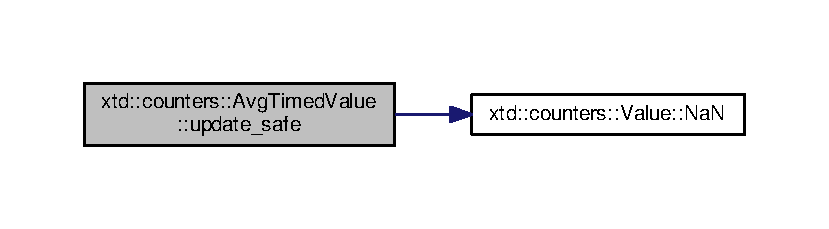
\includegraphics[width=350pt]{classxtd_1_1counters_1_1AvgTimedValue_a1430fd5ff91e960a251b0656c2b5c0ca_cgraph}
\end{center}
\end{figure}




\subsection{Friends And Related Function Documentation}
\hypertarget{classxtd_1_1counters_1_1AvgTimedValue_a93e934ad70d5b32b14beed5572450abf}{\index{xtd\-::counters\-::\-Avg\-Timed\-Value@{xtd\-::counters\-::\-Avg\-Timed\-Value}!Composed@{Composed}}
\index{Composed@{Composed}!xtd::counters::AvgTimedValue@{xtd\-::counters\-::\-Avg\-Timed\-Value}}
\subsubsection[{Composed}]{\setlength{\rightskip}{0pt plus 5cm}friend class {\bf Composed}\hspace{0.3cm}{\ttfamily [friend]}}}\label{classxtd_1_1counters_1_1AvgTimedValue_a93e934ad70d5b32b14beed5572450abf}


Definition at line 21 of file Avg\-Timed\-Value.\-hh.



\subsection{Member Data Documentation}
\hypertarget{classxtd_1_1counters_1_1AvgTimedValue_a6e4edcfa3fcd639b23195119f2b28bd3}{\index{xtd\-::counters\-::\-Avg\-Timed\-Value@{xtd\-::counters\-::\-Avg\-Timed\-Value}!m\-\_\-assert@{m\-\_\-assert}}
\index{m\-\_\-assert@{m\-\_\-assert}!xtd::counters::AvgTimedValue@{xtd\-::counters\-::\-Avg\-Timed\-Value}}
\subsubsection[{m\-\_\-assert}]{\setlength{\rightskip}{0pt plus 5cm}bool xtd\-::counters\-::\-Avg\-Timed\-Value\-::m\-\_\-assert}}\label{classxtd_1_1counters_1_1AvgTimedValue_a6e4edcfa3fcd639b23195119f2b28bd3}


Definition at line 67 of file Avg\-Timed\-Value.\-hh.

\hypertarget{classxtd_1_1counters_1_1AvgTimedValue_ad0b3148989210f269416e5af2169278e}{\index{xtd\-::counters\-::\-Avg\-Timed\-Value@{xtd\-::counters\-::\-Avg\-Timed\-Value}!m\-\_\-global\-Perf@{m\-\_\-global\-Perf}}
\index{m\-\_\-global\-Perf@{m\-\_\-global\-Perf}!xtd::counters::AvgTimedValue@{xtd\-::counters\-::\-Avg\-Timed\-Value}}
\subsubsection[{m\-\_\-global\-Perf}]{\setlength{\rightskip}{0pt plus 5cm}{\bf Freq} xtd\-::counters\-::\-Avg\-Timed\-Value\-::m\-\_\-global\-Perf}}\label{classxtd_1_1counters_1_1AvgTimedValue_ad0b3148989210f269416e5af2169278e}


Definition at line 59 of file Avg\-Timed\-Value.\-hh.

\hypertarget{classxtd_1_1counters_1_1AvgTimedValue_a16f6336d72850b29aa10a97d72309ec4}{\index{xtd\-::counters\-::\-Avg\-Timed\-Value@{xtd\-::counters\-::\-Avg\-Timed\-Value}!m\-\_\-instant\-Perf@{m\-\_\-instant\-Perf}}
\index{m\-\_\-instant\-Perf@{m\-\_\-instant\-Perf}!xtd::counters::AvgTimedValue@{xtd\-::counters\-::\-Avg\-Timed\-Value}}
\subsubsection[{m\-\_\-instant\-Perf}]{\setlength{\rightskip}{0pt plus 5cm}{\bf Instant\-Freq} xtd\-::counters\-::\-Avg\-Timed\-Value\-::m\-\_\-instant\-Perf}}\label{classxtd_1_1counters_1_1AvgTimedValue_a16f6336d72850b29aa10a97d72309ec4}


Definition at line 60 of file Avg\-Timed\-Value.\-hh.

\hypertarget{classxtd_1_1counters_1_1AvgTimedValue_a90ef2640c6d711a3eef2585aaef50afb}{\index{xtd\-::counters\-::\-Avg\-Timed\-Value@{xtd\-::counters\-::\-Avg\-Timed\-Value}!m\-\_\-max@{m\-\_\-max}}
\index{m\-\_\-max@{m\-\_\-max}!xtd::counters::AvgTimedValue@{xtd\-::counters\-::\-Avg\-Timed\-Value}}
\subsubsection[{m\-\_\-max}]{\setlength{\rightskip}{0pt plus 5cm}{\bf Value32} xtd\-::counters\-::\-Avg\-Timed\-Value\-::m\-\_\-max}}\label{classxtd_1_1counters_1_1AvgTimedValue_a90ef2640c6d711a3eef2585aaef50afb}


Definition at line 63 of file Avg\-Timed\-Value.\-hh.

\hypertarget{classxtd_1_1counters_1_1AvgTimedValue_ab0eb52c60a1fe28c6ea148270ca8cc74}{\index{xtd\-::counters\-::\-Avg\-Timed\-Value@{xtd\-::counters\-::\-Avg\-Timed\-Value}!m\-\_\-mean@{m\-\_\-mean}}
\index{m\-\_\-mean@{m\-\_\-mean}!xtd::counters::AvgTimedValue@{xtd\-::counters\-::\-Avg\-Timed\-Value}}
\subsubsection[{m\-\_\-mean}]{\setlength{\rightskip}{0pt plus 5cm}{\bf Value32} xtd\-::counters\-::\-Avg\-Timed\-Value\-::m\-\_\-mean}}\label{classxtd_1_1counters_1_1AvgTimedValue_ab0eb52c60a1fe28c6ea148270ca8cc74}


Definition at line 61 of file Avg\-Timed\-Value.\-hh.

\hypertarget{classxtd_1_1counters_1_1AvgTimedValue_aeed066e7062c73d577033308bc0344bf}{\index{xtd\-::counters\-::\-Avg\-Timed\-Value@{xtd\-::counters\-::\-Avg\-Timed\-Value}!m\-\_\-min@{m\-\_\-min}}
\index{m\-\_\-min@{m\-\_\-min}!xtd::counters::AvgTimedValue@{xtd\-::counters\-::\-Avg\-Timed\-Value}}
\subsubsection[{m\-\_\-min}]{\setlength{\rightskip}{0pt plus 5cm}{\bf Value32} xtd\-::counters\-::\-Avg\-Timed\-Value\-::m\-\_\-min}}\label{classxtd_1_1counters_1_1AvgTimedValue_aeed066e7062c73d577033308bc0344bf}


Definition at line 62 of file Avg\-Timed\-Value.\-hh.

\hypertarget{classxtd_1_1counters_1_1AvgTimedValue_a7a91ad83dade8f67c4df8150ddb33060}{\index{xtd\-::counters\-::\-Avg\-Timed\-Value@{xtd\-::counters\-::\-Avg\-Timed\-Value}!m\-\_\-over\-Threshold@{m\-\_\-over\-Threshold}}
\index{m\-\_\-over\-Threshold@{m\-\_\-over\-Threshold}!xtd::counters::AvgTimedValue@{xtd\-::counters\-::\-Avg\-Timed\-Value}}
\subsubsection[{m\-\_\-over\-Threshold}]{\setlength{\rightskip}{0pt plus 5cm}{\bf Value32} xtd\-::counters\-::\-Avg\-Timed\-Value\-::m\-\_\-over\-Threshold}}\label{classxtd_1_1counters_1_1AvgTimedValue_a7a91ad83dade8f67c4df8150ddb33060}


Definition at line 64 of file Avg\-Timed\-Value.\-hh.

\hypertarget{classxtd_1_1counters_1_1AvgTimedValue_a9f3477cd3eb3fb75f2ba8d75d706eb88}{\index{xtd\-::counters\-::\-Avg\-Timed\-Value@{xtd\-::counters\-::\-Avg\-Timed\-Value}!m\-\_\-reseted@{m\-\_\-reseted}}
\index{m\-\_\-reseted@{m\-\_\-reseted}!xtd::counters::AvgTimedValue@{xtd\-::counters\-::\-Avg\-Timed\-Value}}
\subsubsection[{m\-\_\-reseted}]{\setlength{\rightskip}{0pt plus 5cm}vector$<$uint32\-\_\-t$>$ xtd\-::counters\-::\-Avg\-Timed\-Value\-::m\-\_\-reseted}}\label{classxtd_1_1counters_1_1AvgTimedValue_a9f3477cd3eb3fb75f2ba8d75d706eb88}


Definition at line 58 of file Avg\-Timed\-Value.\-hh.

\hypertarget{classxtd_1_1counters_1_1AvgTimedValue_af33c7f1f69e37ef49e4195de8f4ac6e2}{\index{xtd\-::counters\-::\-Avg\-Timed\-Value@{xtd\-::counters\-::\-Avg\-Timed\-Value}!m\-\_\-samples@{m\-\_\-samples}}
\index{m\-\_\-samples@{m\-\_\-samples}!xtd::counters::AvgTimedValue@{xtd\-::counters\-::\-Avg\-Timed\-Value}}
\subsubsection[{m\-\_\-samples}]{\setlength{\rightskip}{0pt plus 5cm}{\bf t\-\_\-samples} xtd\-::counters\-::\-Avg\-Timed\-Value\-::m\-\_\-samples}}\label{classxtd_1_1counters_1_1AvgTimedValue_af33c7f1f69e37ef49e4195de8f4ac6e2}


Definition at line 56 of file Avg\-Timed\-Value.\-hh.

\hypertarget{classxtd_1_1counters_1_1AvgTimedValue_aff4e550c326e9e16ad2f9e5ff384ae2e}{\index{xtd\-::counters\-::\-Avg\-Timed\-Value@{xtd\-::counters\-::\-Avg\-Timed\-Value}!m\-\_\-start\-Times@{m\-\_\-start\-Times}}
\index{m\-\_\-start\-Times@{m\-\_\-start\-Times}!xtd::counters::AvgTimedValue@{xtd\-::counters\-::\-Avg\-Timed\-Value}}
\subsubsection[{m\-\_\-start\-Times}]{\setlength{\rightskip}{0pt plus 5cm}{\bf t\-\_\-timevect} xtd\-::counters\-::\-Avg\-Timed\-Value\-::m\-\_\-start\-Times}}\label{classxtd_1_1counters_1_1AvgTimedValue_aff4e550c326e9e16ad2f9e5ff384ae2e}


Definition at line 57 of file Avg\-Timed\-Value.\-hh.

\hypertarget{classxtd_1_1counters_1_1AvgTimedValue_a96ae1248a1019b22cf41bae4a47314c2}{\index{xtd\-::counters\-::\-Avg\-Timed\-Value@{xtd\-::counters\-::\-Avg\-Timed\-Value}!m\-\_\-threshold\-Ms@{m\-\_\-threshold\-Ms}}
\index{m\-\_\-threshold\-Ms@{m\-\_\-threshold\-Ms}!xtd::counters::AvgTimedValue@{xtd\-::counters\-::\-Avg\-Timed\-Value}}
\subsubsection[{m\-\_\-threshold\-Ms}]{\setlength{\rightskip}{0pt plus 5cm}const uint32\-\_\-t xtd\-::counters\-::\-Avg\-Timed\-Value\-::m\-\_\-threshold\-Ms}}\label{classxtd_1_1counters_1_1AvgTimedValue_a96ae1248a1019b22cf41bae4a47314c2}


Definition at line 66 of file Avg\-Timed\-Value.\-hh.

\hypertarget{classxtd_1_1counters_1_1AvgTimedValue_a2986c9cf3526f6f86d340dafd25ae04f}{\index{xtd\-::counters\-::\-Avg\-Timed\-Value@{xtd\-::counters\-::\-Avg\-Timed\-Value}!m\-\_\-time\-Delta\-Ms@{m\-\_\-time\-Delta\-Ms}}
\index{m\-\_\-time\-Delta\-Ms@{m\-\_\-time\-Delta\-Ms}!xtd::counters::AvgTimedValue@{xtd\-::counters\-::\-Avg\-Timed\-Value}}
\subsubsection[{m\-\_\-time\-Delta\-Ms}]{\setlength{\rightskip}{0pt plus 5cm}const uint32\-\_\-t xtd\-::counters\-::\-Avg\-Timed\-Value\-::m\-\_\-time\-Delta\-Ms}}\label{classxtd_1_1counters_1_1AvgTimedValue_a2986c9cf3526f6f86d340dafd25ae04f}


Definition at line 65 of file Avg\-Timed\-Value.\-hh.



The documentation for this class was generated from the following files\-:\begin{DoxyCompactItemize}
\item 
/home/travis/build/psycofdj/xtdcpp/counters/src/\hyperlink{AvgTimedValue_8hh}{Avg\-Timed\-Value.\-hh}\item 
/home/travis/build/psycofdj/xtdcpp/counters/src/\hyperlink{AvgTimedValue_8cc}{Avg\-Timed\-Value.\-cc}\end{DoxyCompactItemize}

\hypertarget{classxtd_1_1counters_1_1AvgValue}{}\section{xtd\+:\+:counters\+:\+:Avg\+Value$<$ T\+Type $>$ Class Template Reference}
\label{classxtd_1_1counters_1_1AvgValue}\index{xtd\+::counters\+::\+Avg\+Value$<$ T\+Type $>$@{xtd\+::counters\+::\+Avg\+Value$<$ T\+Type $>$}}


{\ttfamily \#include $<$Avg\+Value.\+hh$>$}



Inheritance diagram for xtd\+:\+:counters\+:\+:Avg\+Value$<$ T\+Type $>$\+:
\nopagebreak
\begin{figure}[H]
\begin{center}
\leavevmode
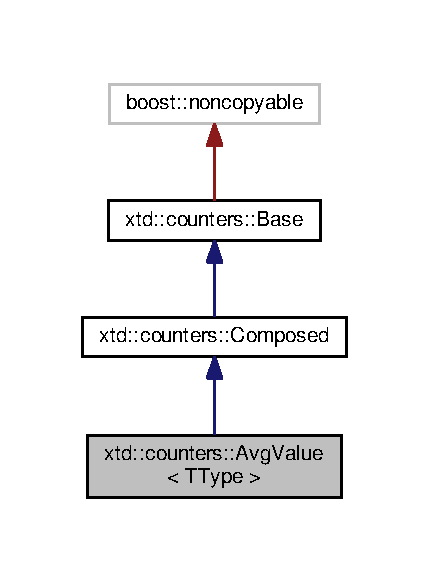
\includegraphics[width=207pt]{classxtd_1_1counters_1_1AvgValue__inherit__graph}
\end{center}
\end{figure}


Collaboration diagram for xtd\+:\+:counters\+:\+:Avg\+Value$<$ T\+Type $>$\+:
\nopagebreak
\begin{figure}[H]
\begin{center}
\leavevmode
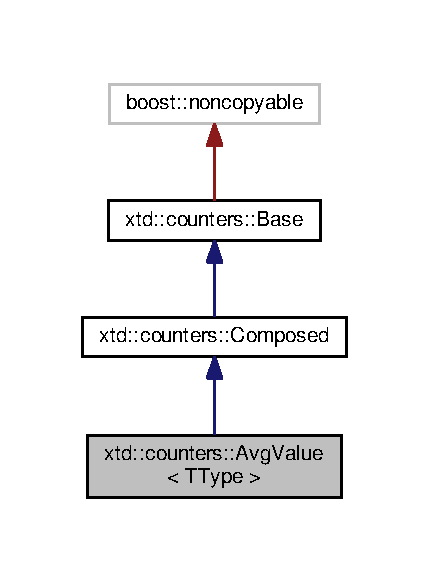
\includegraphics[width=207pt]{classxtd_1_1counters_1_1AvgValue__coll__graph}
\end{center}
\end{figure}
\subsection*{Public Types}
\begin{DoxyCompactItemize}
\item 
typedef boost\+::shared\+\_\+ptr$<$ \hyperlink{classxtd_1_1counters_1_1AvgValue}{Avg\+Value}$<$ T\+Type $>$ $>$ \hyperlink{classxtd_1_1counters_1_1AvgValue_a2186c119cedc1cd9c3a7a7a39e0bdc55}{t\+\_\+sptr}
\end{DoxyCompactItemize}
\subsection*{Public Member Functions}
\begin{DoxyCompactItemize}
\item 
\hyperlink{classxtd_1_1counters_1_1AvgValue_aa6f20ce5b30cc7a781669cd6e4f70a6b}{Avg\+Value} (const string \&p\+\_\+name, uint32\+\_\+t p\+\_\+sampe\+Size=\hyperlink{classxtd_1_1counters_1_1AvgValue_aa65f0400547f2cb940ec9b79cbc3a662}{mcs\+\_\+default\+Sample\+Size})
\item 
virtual \hyperlink{classxtd_1_1counters_1_1AvgValue_ad9e1d371b0787698ebdf0350e58601c8}{$\sim$\+Avg\+Value} (void)
\item 
\hyperlink{classxtd_1_1counters_1_1AvgValue}{Avg\+Value} \& \hyperlink{classxtd_1_1counters_1_1AvgValue_a9605750713e85b4bf2e09e54e46d4e1a}{operator=} (const T\+Type \&p\+\_\+value)
\item 
\hyperlink{classxtd_1_1counters_1_1AvgValue}{Avg\+Value} \& \hyperlink{classxtd_1_1counters_1_1AvgValue_a52054872a2d938baf8c23e1208d7613a}{operator+} (const \hyperlink{classxtd_1_1counters_1_1AvgValue}{Avg\+Value} \&p\+\_\+value)
\end{DoxyCompactItemize}
\subsection*{Static Public Attributes}
\begin{DoxyCompactItemize}
\item 
static const uint32\+\_\+t \hyperlink{classxtd_1_1counters_1_1AvgValue_aa65f0400547f2cb940ec9b79cbc3a662}{mcs\+\_\+default\+Sample\+Size} = 1000
\end{DoxyCompactItemize}
\subsection*{Protected Types}
\begin{DoxyCompactItemize}
\item 
typedef std\+::deque$<$ T\+Type $>$ \hyperlink{classxtd_1_1counters_1_1AvgValue_aa58af8a852f52342b087373414e61878}{t\+\_\+samples}
\end{DoxyCompactItemize}
\subsection*{Protected Member Functions}
\begin{DoxyCompactItemize}
\item 
void \hyperlink{classxtd_1_1counters_1_1AvgValue_a3ad3008fc30f1936e8dd1eef1d62f324}{affect\+\_\+safe} (const T\+Type \&p\+\_\+value)
\item 
void \hyperlink{classxtd_1_1counters_1_1AvgValue_ad0532ed35af8242fabd3a910cc88c543}{add\+\_\+safe} (const \hyperlink{classxtd_1_1counters_1_1AvgValue}{Avg\+Value} \&p\+\_\+value)
\end{DoxyCompactItemize}
\subsection*{Protected Attributes}
\begin{DoxyCompactItemize}
\item 
\hyperlink{classxtd_1_1counters_1_1AvgValue_aa58af8a852f52342b087373414e61878}{t\+\_\+samples} \hyperlink{classxtd_1_1counters_1_1AvgValue_a787afb6a601eb29f48a0fd247524cf84}{m\+\_\+samples}
\item 
\hyperlink{classxtd_1_1counters_1_1Value}{Value}$<$ T\+Type $>$ \hyperlink{classxtd_1_1counters_1_1AvgValue_afa1908ab38d3deef50e1169b1cc20f6c}{m\+\_\+mean}
\item 
\hyperlink{classxtd_1_1counters_1_1Value}{Value}$<$ T\+Type $>$ \hyperlink{classxtd_1_1counters_1_1AvgValue_a8e217891d937894812b5edfcf6a5ce0e}{m\+\_\+min}
\item 
\hyperlink{classxtd_1_1counters_1_1Value}{Value}$<$ T\+Type $>$ \hyperlink{classxtd_1_1counters_1_1AvgValue_a9ee9567a0a95cf6b579c13329f21f0d5}{m\+\_\+max}
\item 
uint32\+\_\+t \hyperlink{classxtd_1_1counters_1_1AvgValue_aba4c4022706bda9bfdedea3cb9c3647a}{m\+\_\+nb\+Event}
\item 
const uint32\+\_\+t \hyperlink{classxtd_1_1counters_1_1AvgValue_a85edafd4829b5aa5be6562cadd8e4764}{m\+\_\+sample\+Size}
\end{DoxyCompactItemize}
\subsection*{Friends}
\begin{DoxyCompactItemize}
\item 
class \hyperlink{classxtd_1_1counters_1_1AvgValue_a93e934ad70d5b32b14beed5572450abf}{Composed}
\end{DoxyCompactItemize}


\subsection{Detailed Description}
\subsubsection*{template$<$typename T\+Type$>$\\*
class xtd\+::counters\+::\+Avg\+Value$<$ T\+Type $>$}



Definition at line 14 of file Avg\+Value.\+hh.



\subsection{Member Typedef Documentation}
\index{xtd\+::counters\+::\+Avg\+Value@{xtd\+::counters\+::\+Avg\+Value}!t\+\_\+samples@{t\+\_\+samples}}
\index{t\+\_\+samples@{t\+\_\+samples}!xtd\+::counters\+::\+Avg\+Value@{xtd\+::counters\+::\+Avg\+Value}}
\subsubsection[{\texorpdfstring{t\+\_\+samples}{t_samples}}]{\setlength{\rightskip}{0pt plus 5cm}template$<$typename T\+Type$>$ typedef std\+::deque$<$T\+Type$>$ {\bf xtd\+::counters\+::\+Avg\+Value}$<$ T\+Type $>$\+::{\bf t\+\_\+samples}\hspace{0.3cm}{\ttfamily [protected]}}\hypertarget{classxtd_1_1counters_1_1AvgValue_aa58af8a852f52342b087373414e61878}{}\label{classxtd_1_1counters_1_1AvgValue_aa58af8a852f52342b087373414e61878}


Definition at line 22 of file Avg\+Value.\+hh.

\index{xtd\+::counters\+::\+Avg\+Value@{xtd\+::counters\+::\+Avg\+Value}!t\+\_\+sptr@{t\+\_\+sptr}}
\index{t\+\_\+sptr@{t\+\_\+sptr}!xtd\+::counters\+::\+Avg\+Value@{xtd\+::counters\+::\+Avg\+Value}}
\subsubsection[{\texorpdfstring{t\+\_\+sptr}{t_sptr}}]{\setlength{\rightskip}{0pt plus 5cm}template$<$typename T\+Type$>$ typedef boost\+::shared\+\_\+ptr$<${\bf Avg\+Value}$<$T\+Type$>$ $>$ {\bf xtd\+::counters\+::\+Avg\+Value}$<$ T\+Type $>$\+::{\bf t\+\_\+sptr}}\hypertarget{classxtd_1_1counters_1_1AvgValue_a2186c119cedc1cd9c3a7a7a39e0bdc55}{}\label{classxtd_1_1counters_1_1AvgValue_a2186c119cedc1cd9c3a7a7a39e0bdc55}


Definition at line 19 of file Avg\+Value.\+hh.



\subsection{Constructor \& Destructor Documentation}
\index{xtd\+::counters\+::\+Avg\+Value@{xtd\+::counters\+::\+Avg\+Value}!Avg\+Value@{Avg\+Value}}
\index{Avg\+Value@{Avg\+Value}!xtd\+::counters\+::\+Avg\+Value@{xtd\+::counters\+::\+Avg\+Value}}
\subsubsection[{\texorpdfstring{Avg\+Value(const string \&p\+\_\+name, uint32\+\_\+t p\+\_\+sampe\+Size=mcs\+\_\+default\+Sample\+Size)}{AvgValue(const string &p_name, uint32_t p_sampeSize=mcs_defaultSampleSize)}}]{\setlength{\rightskip}{0pt plus 5cm}template$<$typename T\+Type$>$ {\bf xtd\+::counters\+::\+Avg\+Value}$<$ T\+Type $>$\+::{\bf Avg\+Value} (
\begin{DoxyParamCaption}
\item[{const string \&}]{p\+\_\+name, }
\item[{uint32\+\_\+t}]{p\+\_\+sampe\+Size = {\ttfamily {\bf mcs\+\_\+default\+Sample\+Size}}}
\end{DoxyParamCaption}
)}\hypertarget{classxtd_1_1counters_1_1AvgValue_aa6f20ce5b30cc7a781669cd6e4f70a6b}{}\label{classxtd_1_1counters_1_1AvgValue_aa6f20ce5b30cc7a781669cd6e4f70a6b}
\index{xtd\+::counters\+::\+Avg\+Value@{xtd\+::counters\+::\+Avg\+Value}!````~Avg\+Value@{$\sim$\+Avg\+Value}}
\index{````~Avg\+Value@{$\sim$\+Avg\+Value}!xtd\+::counters\+::\+Avg\+Value@{xtd\+::counters\+::\+Avg\+Value}}
\subsubsection[{\texorpdfstring{$\sim$\+Avg\+Value(void)}{~AvgValue(void)}}]{\setlength{\rightskip}{0pt plus 5cm}template$<$typename T\+Type$>$ virtual {\bf xtd\+::counters\+::\+Avg\+Value}$<$ T\+Type $>$\+::$\sim${\bf Avg\+Value} (
\begin{DoxyParamCaption}
\item[{void}]{}
\end{DoxyParamCaption}
)\hspace{0.3cm}{\ttfamily [inline]}, {\ttfamily [virtual]}}\hypertarget{classxtd_1_1counters_1_1AvgValue_ad9e1d371b0787698ebdf0350e58601c8}{}\label{classxtd_1_1counters_1_1AvgValue_ad9e1d371b0787698ebdf0350e58601c8}


Definition at line 30 of file Avg\+Value.\+hh.


\begin{DoxyCode}
30 \{\};
\end{DoxyCode}


\subsection{Member Function Documentation}
\index{xtd\+::counters\+::\+Avg\+Value@{xtd\+::counters\+::\+Avg\+Value}!add\+\_\+safe@{add\+\_\+safe}}
\index{add\+\_\+safe@{add\+\_\+safe}!xtd\+::counters\+::\+Avg\+Value@{xtd\+::counters\+::\+Avg\+Value}}
\subsubsection[{\texorpdfstring{add\+\_\+safe(const Avg\+Value \&p\+\_\+value)}{add_safe(const AvgValue &p_value)}}]{\setlength{\rightskip}{0pt plus 5cm}template$<$typename T\+Type$>$ void {\bf xtd\+::counters\+::\+Avg\+Value}$<$ T\+Type $>$\+::add\+\_\+safe (
\begin{DoxyParamCaption}
\item[{const {\bf Avg\+Value}$<$ T\+Type $>$ \&}]{p\+\_\+value}
\end{DoxyParamCaption}
)\hspace{0.3cm}{\ttfamily [protected]}}\hypertarget{classxtd_1_1counters_1_1AvgValue_ad0532ed35af8242fabd3a910cc88c543}{}\label{classxtd_1_1counters_1_1AvgValue_ad0532ed35af8242fabd3a910cc88c543}


Here is the caller graph for this function\+:
\nopagebreak
\begin{figure}[H]
\begin{center}
\leavevmode
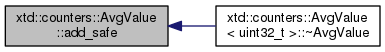
\includegraphics[width=350pt]{classxtd_1_1counters_1_1AvgValue_ad0532ed35af8242fabd3a910cc88c543_icgraph}
\end{center}
\end{figure}


\index{xtd\+::counters\+::\+Avg\+Value@{xtd\+::counters\+::\+Avg\+Value}!affect\+\_\+safe@{affect\+\_\+safe}}
\index{affect\+\_\+safe@{affect\+\_\+safe}!xtd\+::counters\+::\+Avg\+Value@{xtd\+::counters\+::\+Avg\+Value}}
\subsubsection[{\texorpdfstring{affect\+\_\+safe(const T\+Type \&p\+\_\+value)}{affect_safe(const TType &p_value)}}]{\setlength{\rightskip}{0pt plus 5cm}template$<$typename T\+Type$>$ void {\bf xtd\+::counters\+::\+Avg\+Value}$<$ T\+Type $>$\+::affect\+\_\+safe (
\begin{DoxyParamCaption}
\item[{const T\+Type \&}]{p\+\_\+value}
\end{DoxyParamCaption}
)\hspace{0.3cm}{\ttfamily [protected]}}\hypertarget{classxtd_1_1counters_1_1AvgValue_a3ad3008fc30f1936e8dd1eef1d62f324}{}\label{classxtd_1_1counters_1_1AvgValue_a3ad3008fc30f1936e8dd1eef1d62f324}


Here is the caller graph for this function\+:
\nopagebreak
\begin{figure}[H]
\begin{center}
\leavevmode
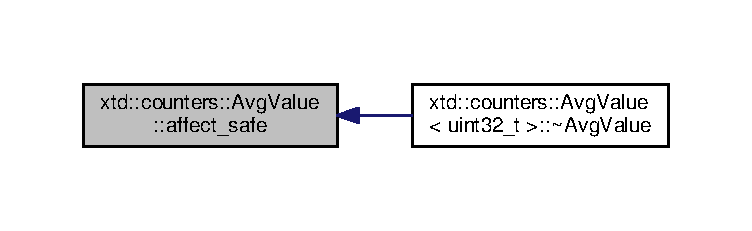
\includegraphics[width=350pt]{classxtd_1_1counters_1_1AvgValue_a3ad3008fc30f1936e8dd1eef1d62f324_icgraph}
\end{center}
\end{figure}


\index{xtd\+::counters\+::\+Avg\+Value@{xtd\+::counters\+::\+Avg\+Value}!operator+@{operator+}}
\index{operator+@{operator+}!xtd\+::counters\+::\+Avg\+Value@{xtd\+::counters\+::\+Avg\+Value}}
\subsubsection[{\texorpdfstring{operator+(const Avg\+Value \&p\+\_\+value)}{operator+(const AvgValue &p_value)}}]{\setlength{\rightskip}{0pt plus 5cm}template$<$typename T\+Type$>$ {\bf Avg\+Value}\& {\bf xtd\+::counters\+::\+Avg\+Value}$<$ T\+Type $>$\+::operator+ (
\begin{DoxyParamCaption}
\item[{const {\bf Avg\+Value}$<$ T\+Type $>$ \&}]{p\+\_\+value}
\end{DoxyParamCaption}
)}\hypertarget{classxtd_1_1counters_1_1AvgValue_a52054872a2d938baf8c23e1208d7613a}{}\label{classxtd_1_1counters_1_1AvgValue_a52054872a2d938baf8c23e1208d7613a}


Here is the caller graph for this function\+:
\nopagebreak
\begin{figure}[H]
\begin{center}
\leavevmode
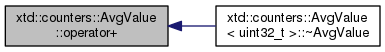
\includegraphics[width=350pt]{classxtd_1_1counters_1_1AvgValue_a52054872a2d938baf8c23e1208d7613a_icgraph}
\end{center}
\end{figure}


\index{xtd\+::counters\+::\+Avg\+Value@{xtd\+::counters\+::\+Avg\+Value}!operator=@{operator=}}
\index{operator=@{operator=}!xtd\+::counters\+::\+Avg\+Value@{xtd\+::counters\+::\+Avg\+Value}}
\subsubsection[{\texorpdfstring{operator=(const T\+Type \&p\+\_\+value)}{operator=(const TType &p_value)}}]{\setlength{\rightskip}{0pt plus 5cm}template$<$typename T\+Type$>$ {\bf Avg\+Value}\& {\bf xtd\+::counters\+::\+Avg\+Value}$<$ T\+Type $>$\+::operator= (
\begin{DoxyParamCaption}
\item[{const T\+Type \&}]{p\+\_\+value}
\end{DoxyParamCaption}
)}\hypertarget{classxtd_1_1counters_1_1AvgValue_a9605750713e85b4bf2e09e54e46d4e1a}{}\label{classxtd_1_1counters_1_1AvgValue_a9605750713e85b4bf2e09e54e46d4e1a}


Here is the caller graph for this function\+:
\nopagebreak
\begin{figure}[H]
\begin{center}
\leavevmode
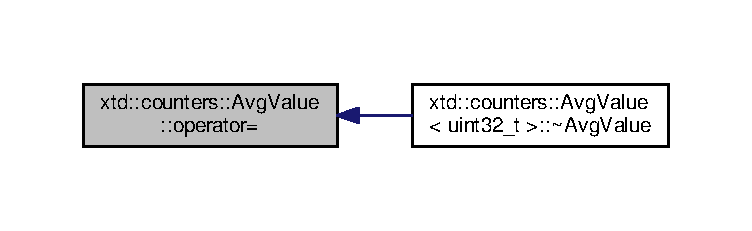
\includegraphics[width=350pt]{classxtd_1_1counters_1_1AvgValue_a9605750713e85b4bf2e09e54e46d4e1a_icgraph}
\end{center}
\end{figure}




\subsection{Friends And Related Function Documentation}
\index{xtd\+::counters\+::\+Avg\+Value@{xtd\+::counters\+::\+Avg\+Value}!Composed@{Composed}}
\index{Composed@{Composed}!xtd\+::counters\+::\+Avg\+Value@{xtd\+::counters\+::\+Avg\+Value}}
\subsubsection[{\texorpdfstring{Composed}{Composed}}]{\setlength{\rightskip}{0pt plus 5cm}template$<$typename T\+Type$>$ friend class {\bf Composed}\hspace{0.3cm}{\ttfamily [friend]}}\hypertarget{classxtd_1_1counters_1_1AvgValue_a93e934ad70d5b32b14beed5572450abf}{}\label{classxtd_1_1counters_1_1AvgValue_a93e934ad70d5b32b14beed5572450abf}


Definition at line 16 of file Avg\+Value.\+hh.



\subsection{Member Data Documentation}
\index{xtd\+::counters\+::\+Avg\+Value@{xtd\+::counters\+::\+Avg\+Value}!m\+\_\+max@{m\+\_\+max}}
\index{m\+\_\+max@{m\+\_\+max}!xtd\+::counters\+::\+Avg\+Value@{xtd\+::counters\+::\+Avg\+Value}}
\subsubsection[{\texorpdfstring{m\+\_\+max}{m_max}}]{\setlength{\rightskip}{0pt plus 5cm}template$<$typename T\+Type$>$ {\bf Value}$<$T\+Type$>$ {\bf xtd\+::counters\+::\+Avg\+Value}$<$ T\+Type $>$\+::m\+\_\+max\hspace{0.3cm}{\ttfamily [protected]}}\hypertarget{classxtd_1_1counters_1_1AvgValue_a9ee9567a0a95cf6b579c13329f21f0d5}{}\label{classxtd_1_1counters_1_1AvgValue_a9ee9567a0a95cf6b579c13329f21f0d5}


Definition at line 44 of file Avg\+Value.\+hh.

\index{xtd\+::counters\+::\+Avg\+Value@{xtd\+::counters\+::\+Avg\+Value}!m\+\_\+mean@{m\+\_\+mean}}
\index{m\+\_\+mean@{m\+\_\+mean}!xtd\+::counters\+::\+Avg\+Value@{xtd\+::counters\+::\+Avg\+Value}}
\subsubsection[{\texorpdfstring{m\+\_\+mean}{m_mean}}]{\setlength{\rightskip}{0pt plus 5cm}template$<$typename T\+Type$>$ {\bf Value}$<$T\+Type$>$ {\bf xtd\+::counters\+::\+Avg\+Value}$<$ T\+Type $>$\+::m\+\_\+mean\hspace{0.3cm}{\ttfamily [protected]}}\hypertarget{classxtd_1_1counters_1_1AvgValue_afa1908ab38d3deef50e1169b1cc20f6c}{}\label{classxtd_1_1counters_1_1AvgValue_afa1908ab38d3deef50e1169b1cc20f6c}


Definition at line 42 of file Avg\+Value.\+hh.

\index{xtd\+::counters\+::\+Avg\+Value@{xtd\+::counters\+::\+Avg\+Value}!m\+\_\+min@{m\+\_\+min}}
\index{m\+\_\+min@{m\+\_\+min}!xtd\+::counters\+::\+Avg\+Value@{xtd\+::counters\+::\+Avg\+Value}}
\subsubsection[{\texorpdfstring{m\+\_\+min}{m_min}}]{\setlength{\rightskip}{0pt plus 5cm}template$<$typename T\+Type$>$ {\bf Value}$<$T\+Type$>$ {\bf xtd\+::counters\+::\+Avg\+Value}$<$ T\+Type $>$\+::m\+\_\+min\hspace{0.3cm}{\ttfamily [protected]}}\hypertarget{classxtd_1_1counters_1_1AvgValue_a8e217891d937894812b5edfcf6a5ce0e}{}\label{classxtd_1_1counters_1_1AvgValue_a8e217891d937894812b5edfcf6a5ce0e}


Definition at line 43 of file Avg\+Value.\+hh.

\index{xtd\+::counters\+::\+Avg\+Value@{xtd\+::counters\+::\+Avg\+Value}!m\+\_\+nb\+Event@{m\+\_\+nb\+Event}}
\index{m\+\_\+nb\+Event@{m\+\_\+nb\+Event}!xtd\+::counters\+::\+Avg\+Value@{xtd\+::counters\+::\+Avg\+Value}}
\subsubsection[{\texorpdfstring{m\+\_\+nb\+Event}{m_nbEvent}}]{\setlength{\rightskip}{0pt plus 5cm}template$<$typename T\+Type$>$ uint32\+\_\+t {\bf xtd\+::counters\+::\+Avg\+Value}$<$ T\+Type $>$\+::m\+\_\+nb\+Event\hspace{0.3cm}{\ttfamily [protected]}}\hypertarget{classxtd_1_1counters_1_1AvgValue_aba4c4022706bda9bfdedea3cb9c3647a}{}\label{classxtd_1_1counters_1_1AvgValue_aba4c4022706bda9bfdedea3cb9c3647a}


Definition at line 45 of file Avg\+Value.\+hh.

\index{xtd\+::counters\+::\+Avg\+Value@{xtd\+::counters\+::\+Avg\+Value}!m\+\_\+samples@{m\+\_\+samples}}
\index{m\+\_\+samples@{m\+\_\+samples}!xtd\+::counters\+::\+Avg\+Value@{xtd\+::counters\+::\+Avg\+Value}}
\subsubsection[{\texorpdfstring{m\+\_\+samples}{m_samples}}]{\setlength{\rightskip}{0pt plus 5cm}template$<$typename T\+Type$>$ {\bf t\+\_\+samples} {\bf xtd\+::counters\+::\+Avg\+Value}$<$ T\+Type $>$\+::m\+\_\+samples\hspace{0.3cm}{\ttfamily [protected]}}\hypertarget{classxtd_1_1counters_1_1AvgValue_a787afb6a601eb29f48a0fd247524cf84}{}\label{classxtd_1_1counters_1_1AvgValue_a787afb6a601eb29f48a0fd247524cf84}


Definition at line 41 of file Avg\+Value.\+hh.

\index{xtd\+::counters\+::\+Avg\+Value@{xtd\+::counters\+::\+Avg\+Value}!m\+\_\+sample\+Size@{m\+\_\+sample\+Size}}
\index{m\+\_\+sample\+Size@{m\+\_\+sample\+Size}!xtd\+::counters\+::\+Avg\+Value@{xtd\+::counters\+::\+Avg\+Value}}
\subsubsection[{\texorpdfstring{m\+\_\+sample\+Size}{m_sampleSize}}]{\setlength{\rightskip}{0pt plus 5cm}template$<$typename T\+Type$>$ const uint32\+\_\+t {\bf xtd\+::counters\+::\+Avg\+Value}$<$ T\+Type $>$\+::m\+\_\+sample\+Size\hspace{0.3cm}{\ttfamily [protected]}}\hypertarget{classxtd_1_1counters_1_1AvgValue_a85edafd4829b5aa5be6562cadd8e4764}{}\label{classxtd_1_1counters_1_1AvgValue_a85edafd4829b5aa5be6562cadd8e4764}


Definition at line 47 of file Avg\+Value.\+hh.

\index{xtd\+::counters\+::\+Avg\+Value@{xtd\+::counters\+::\+Avg\+Value}!mcs\+\_\+default\+Sample\+Size@{mcs\+\_\+default\+Sample\+Size}}
\index{mcs\+\_\+default\+Sample\+Size@{mcs\+\_\+default\+Sample\+Size}!xtd\+::counters\+::\+Avg\+Value@{xtd\+::counters\+::\+Avg\+Value}}
\subsubsection[{\texorpdfstring{mcs\+\_\+default\+Sample\+Size}{mcs_defaultSampleSize}}]{\setlength{\rightskip}{0pt plus 5cm}template$<$typename T\+Type$>$ const uint32\+\_\+t {\bf xtd\+::counters\+::\+Avg\+Value}$<$ T\+Type $>$\+::mcs\+\_\+default\+Sample\+Size = 1000\hspace{0.3cm}{\ttfamily [static]}}\hypertarget{classxtd_1_1counters_1_1AvgValue_aa65f0400547f2cb940ec9b79cbc3a662}{}\label{classxtd_1_1counters_1_1AvgValue_aa65f0400547f2cb940ec9b79cbc3a662}


Definition at line 25 of file Avg\+Value.\+hh.



The documentation for this class was generated from the following file\+:\begin{DoxyCompactItemize}
\item 
/home/psyco/dev/xtdcpp/counters/src/\hyperlink{AvgValue_8hh}{Avg\+Value.\+hh}\end{DoxyCompactItemize}

\hypertarget{classxtd_1_1counters_1_1Base}{}\section{xtd\+:\+:counters\+:\+:Base Class Reference}
\label{classxtd_1_1counters_1_1Base}\index{xtd\+::counters\+::\+Base@{xtd\+::counters\+::\+Base}}


{\ttfamily \#include $<$Base.\+hh$>$}



Inheritance diagram for xtd\+:\+:counters\+:\+:Base\+:
\nopagebreak
\begin{figure}[H]
\begin{center}
\leavevmode
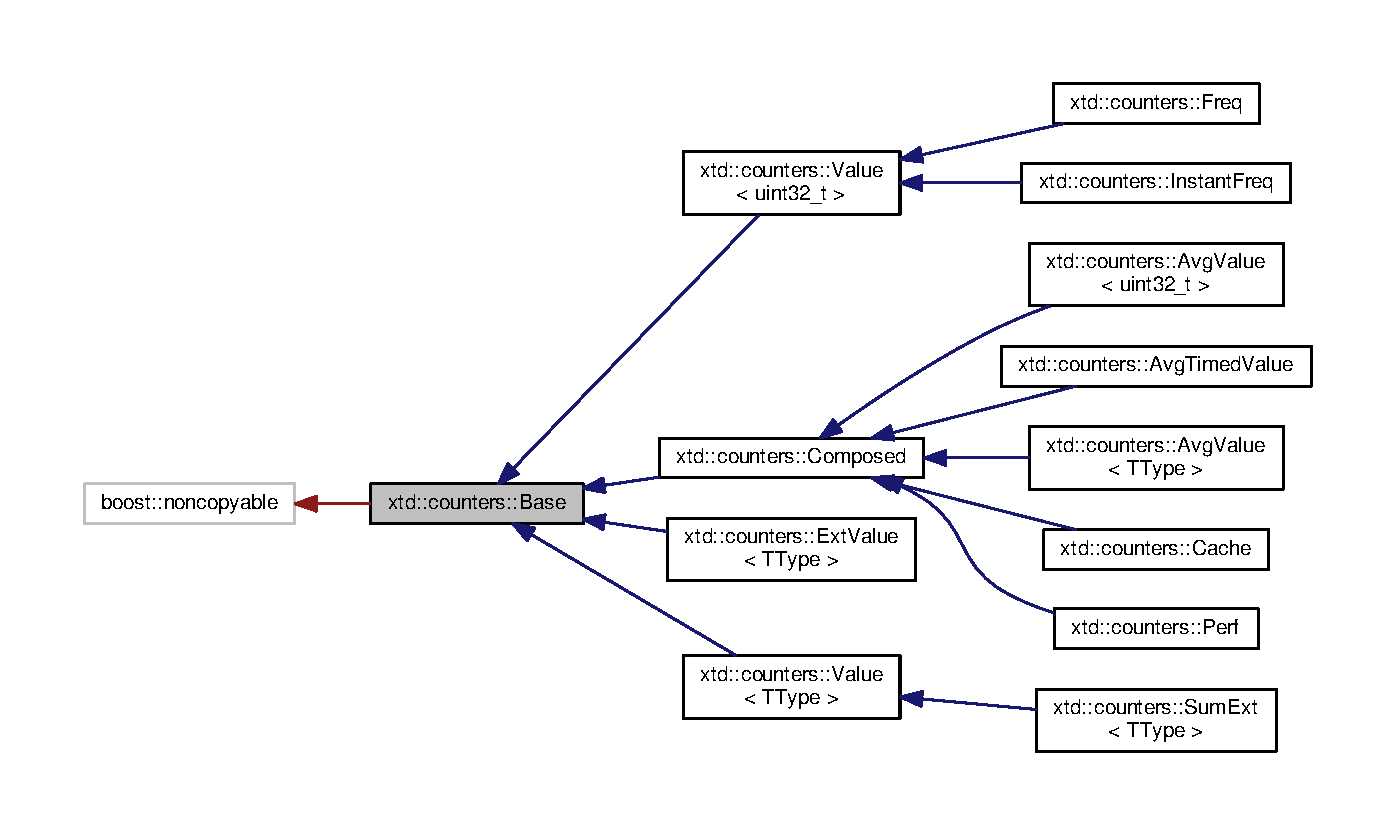
\includegraphics[width=350pt]{classxtd_1_1counters_1_1Base__inherit__graph}
\end{center}
\end{figure}


Collaboration diagram for xtd\+:\+:counters\+:\+:Base\+:
\nopagebreak
\begin{figure}[H]
\begin{center}
\leavevmode
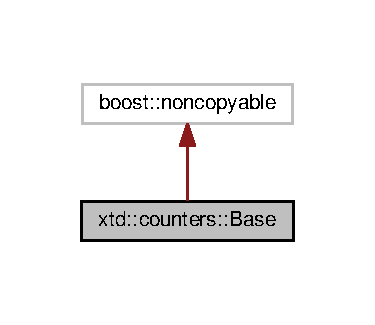
\includegraphics[width=182pt]{classxtd_1_1counters_1_1Base__coll__graph}
\end{center}
\end{figure}
\subsection*{Public Types}
\begin{DoxyCompactItemize}
\item 
typedef boost\+::shared\+\_\+ptr$<$ \hyperlink{classxtd_1_1counters_1_1Base}{Base} $>$ \hyperlink{classxtd_1_1counters_1_1Base_aa0ea634f1a5e3df87418566a3e8fcbd6}{t\+\_\+sptr}
\item 
typedef map$<$ string, string $>$ \hyperlink{classxtd_1_1counters_1_1Base_a8bb7d024911a4c454c003a18e330d268}{t\+\_\+data}
\end{DoxyCompactItemize}
\subsection*{Public Member Functions}
\begin{DoxyCompactItemize}
\item 
\hyperlink{classxtd_1_1counters_1_1Base_ab370a97f3a40bd529e871daedfce60c7}{Base} (const string \&p\+\_\+name)
\item 
virtual \hyperlink{classxtd_1_1counters_1_1Base_aa2bddc0c397ef1e77eff98969ba3bc7d}{$\sim$\+Base} (void)
\item 
void \hyperlink{classxtd_1_1counters_1_1Base_a0c743f0686dc24bada97c2ed31238c02}{visit} (\hyperlink{classxtd_1_1counters_1_1Visitor}{Visitor} \&p\+\_\+visitor) const 
\item 
void \hyperlink{classxtd_1_1counters_1_1Base_a5ba0d495403ba1ca4e1c6c30d8038dad}{update} (void)
\item 
const string \& \hyperlink{classxtd_1_1counters_1_1Base_a64ef0c0b30b420384494fd06c535f84d}{get\+Name} (void) const 
\end{DoxyCompactItemize}
\subsection*{Protected Member Functions}
\begin{DoxyCompactItemize}
\item 
virtual void \hyperlink{classxtd_1_1counters_1_1Base_a8b3d10c9fb2bea1d240f887bbe4008ea}{update\+\_\+safe} (void)
\item 
virtual void \hyperlink{classxtd_1_1counters_1_1Base_a0b8f3bdc6880dc03da750aa815dfdf0b}{visit\+\_\+safe} (\hyperlink{classxtd_1_1counters_1_1Visitor}{Visitor} \&p\+\_\+visitor) const =0
\end{DoxyCompactItemize}
\subsection*{Protected Attributes}
\begin{DoxyCompactItemize}
\item 
string \hyperlink{classxtd_1_1counters_1_1Base_ab07d4a6071bfa8263b24d5992bca6960}{m\+\_\+name}
\item 
boost\+::mutex \hyperlink{classxtd_1_1counters_1_1Base_aeeac2ffcae02eb6341418d708188a353}{m\+\_\+mutex}
\end{DoxyCompactItemize}
\subsection*{Friends}
\begin{DoxyCompactItemize}
\item 
class \hyperlink{classxtd_1_1counters_1_1Base_a93e934ad70d5b32b14beed5572450abf}{Composed}
\end{DoxyCompactItemize}


\subsection{Detailed Description}


Definition at line 13 of file Base.\+hh.



\subsection{Member Typedef Documentation}
\index{xtd\+::counters\+::\+Base@{xtd\+::counters\+::\+Base}!t\+\_\+data@{t\+\_\+data}}
\index{t\+\_\+data@{t\+\_\+data}!xtd\+::counters\+::\+Base@{xtd\+::counters\+::\+Base}}
\subsubsection[{\texorpdfstring{t\+\_\+data}{t_data}}]{\setlength{\rightskip}{0pt plus 5cm}typedef map$<$string, string$>$ {\bf xtd\+::counters\+::\+Base\+::t\+\_\+data}}\hypertarget{classxtd_1_1counters_1_1Base_a8bb7d024911a4c454c003a18e330d268}{}\label{classxtd_1_1counters_1_1Base_a8bb7d024911a4c454c003a18e330d268}


Definition at line 19 of file Base.\+hh.

\index{xtd\+::counters\+::\+Base@{xtd\+::counters\+::\+Base}!t\+\_\+sptr@{t\+\_\+sptr}}
\index{t\+\_\+sptr@{t\+\_\+sptr}!xtd\+::counters\+::\+Base@{xtd\+::counters\+::\+Base}}
\subsubsection[{\texorpdfstring{t\+\_\+sptr}{t_sptr}}]{\setlength{\rightskip}{0pt plus 5cm}typedef boost\+::shared\+\_\+ptr$<${\bf Base}$>$ {\bf xtd\+::counters\+::\+Base\+::t\+\_\+sptr}}\hypertarget{classxtd_1_1counters_1_1Base_aa0ea634f1a5e3df87418566a3e8fcbd6}{}\label{classxtd_1_1counters_1_1Base_aa0ea634f1a5e3df87418566a3e8fcbd6}


Definition at line 18 of file Base.\+hh.



\subsection{Constructor \& Destructor Documentation}
\index{xtd\+::counters\+::\+Base@{xtd\+::counters\+::\+Base}!Base@{Base}}
\index{Base@{Base}!xtd\+::counters\+::\+Base@{xtd\+::counters\+::\+Base}}
\subsubsection[{\texorpdfstring{Base(const string \&p\+\_\+name)}{Base(const string &p_name)}}]{\setlength{\rightskip}{0pt plus 5cm}xtd\+::counters\+::\+Base\+::\+Base (
\begin{DoxyParamCaption}
\item[{const string \&}]{p\+\_\+name}
\end{DoxyParamCaption}
)}\hypertarget{classxtd_1_1counters_1_1Base_ab370a97f3a40bd529e871daedfce60c7}{}\label{classxtd_1_1counters_1_1Base_ab370a97f3a40bd529e871daedfce60c7}


Definition at line 7 of file Base.\+cc.


\begin{DoxyCode}
7                                :
8   \hyperlink{classxtd_1_1counters_1_1Base_ab07d4a6071bfa8263b24d5992bca6960}{m\_name}(p\_name)
9 \{
10 \}
\end{DoxyCode}
\index{xtd\+::counters\+::\+Base@{xtd\+::counters\+::\+Base}!````~Base@{$\sim$\+Base}}
\index{````~Base@{$\sim$\+Base}!xtd\+::counters\+::\+Base@{xtd\+::counters\+::\+Base}}
\subsubsection[{\texorpdfstring{$\sim$\+Base(void)}{~Base(void)}}]{\setlength{\rightskip}{0pt plus 5cm}xtd\+::counters\+::\+Base\+::$\sim$\+Base (
\begin{DoxyParamCaption}
\item[{void}]{}
\end{DoxyParamCaption}
)\hspace{0.3cm}{\ttfamily [virtual]}}\hypertarget{classxtd_1_1counters_1_1Base_aa2bddc0c397ef1e77eff98969ba3bc7d}{}\label{classxtd_1_1counters_1_1Base_aa2bddc0c397ef1e77eff98969ba3bc7d}


Definition at line 12 of file Base.\+cc.


\begin{DoxyCode}
13 \{
14 \}
\end{DoxyCode}


\subsection{Member Function Documentation}
\index{xtd\+::counters\+::\+Base@{xtd\+::counters\+::\+Base}!get\+Name@{get\+Name}}
\index{get\+Name@{get\+Name}!xtd\+::counters\+::\+Base@{xtd\+::counters\+::\+Base}}
\subsubsection[{\texorpdfstring{get\+Name(void) const }{getName(void) const }}]{\setlength{\rightskip}{0pt plus 5cm}const string \& xtd\+::counters\+::\+Base\+::get\+Name (
\begin{DoxyParamCaption}
\item[{void}]{}
\end{DoxyParamCaption}
) const}\hypertarget{classxtd_1_1counters_1_1Base_a64ef0c0b30b420384494fd06c535f84d}{}\label{classxtd_1_1counters_1_1Base_a64ef0c0b30b420384494fd06c535f84d}


Definition at line 37 of file Base.\+cc.


\begin{DoxyCode}
38 \{
39   \textcolor{keywordflow}{return} \hyperlink{classxtd_1_1counters_1_1Base_ab07d4a6071bfa8263b24d5992bca6960}{m\_name};
40 \}
\end{DoxyCode}
\index{xtd\+::counters\+::\+Base@{xtd\+::counters\+::\+Base}!update@{update}}
\index{update@{update}!xtd\+::counters\+::\+Base@{xtd\+::counters\+::\+Base}}
\subsubsection[{\texorpdfstring{update(void)}{update(void)}}]{\setlength{\rightskip}{0pt plus 5cm}void xtd\+::counters\+::\+Base\+::update (
\begin{DoxyParamCaption}
\item[{void}]{}
\end{DoxyParamCaption}
)}\hypertarget{classxtd_1_1counters_1_1Base_a5ba0d495403ba1ca4e1c6c30d8038dad}{}\label{classxtd_1_1counters_1_1Base_a5ba0d495403ba1ca4e1c6c30d8038dad}


Definition at line 25 of file Base.\+cc.


\begin{DoxyCode}
26 \{
27   boost::mutex::scoped\_lock l\_lock(\hyperlink{classxtd_1_1counters_1_1Base_aeeac2ffcae02eb6341418d708188a353}{m\_mutex});
28   \hyperlink{classxtd_1_1counters_1_1Base_a8b3d10c9fb2bea1d240f887bbe4008ea}{update\_safe}();
29 \}
\end{DoxyCode}


Here is the call graph for this function\+:
\nopagebreak
\begin{figure}[H]
\begin{center}
\leavevmode
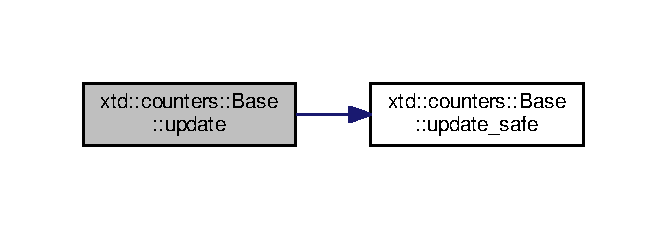
\includegraphics[width=320pt]{classxtd_1_1counters_1_1Base_a5ba0d495403ba1ca4e1c6c30d8038dad_cgraph}
\end{center}
\end{figure}




Here is the caller graph for this function\+:
\nopagebreak
\begin{figure}[H]
\begin{center}
\leavevmode
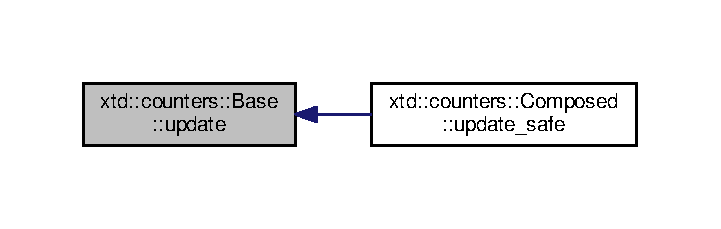
\includegraphics[width=350pt]{classxtd_1_1counters_1_1Base_a5ba0d495403ba1ca4e1c6c30d8038dad_icgraph}
\end{center}
\end{figure}


\index{xtd\+::counters\+::\+Base@{xtd\+::counters\+::\+Base}!update\+\_\+safe@{update\+\_\+safe}}
\index{update\+\_\+safe@{update\+\_\+safe}!xtd\+::counters\+::\+Base@{xtd\+::counters\+::\+Base}}
\subsubsection[{\texorpdfstring{update\+\_\+safe(void)}{update_safe(void)}}]{\setlength{\rightskip}{0pt plus 5cm}void xtd\+::counters\+::\+Base\+::update\+\_\+safe (
\begin{DoxyParamCaption}
\item[{void}]{}
\end{DoxyParamCaption}
)\hspace{0.3cm}{\ttfamily [protected]}, {\ttfamily [virtual]}}\hypertarget{classxtd_1_1counters_1_1Base_a8b3d10c9fb2bea1d240f887bbe4008ea}{}\label{classxtd_1_1counters_1_1Base_a8b3d10c9fb2bea1d240f887bbe4008ea}


Reimplemented in \hyperlink{classxtd_1_1counters_1_1AvgTimedValue_a1430fd5ff91e960a251b0656c2b5c0ca}{xtd\+::counters\+::\+Avg\+Timed\+Value}, \hyperlink{classxtd_1_1counters_1_1InstantFreq_a2e4629f5a835d7b52425a72f25dcd4d2}{xtd\+::counters\+::\+Instant\+Freq}, \hyperlink{classxtd_1_1counters_1_1SumExt_a1f3c5d348aa4b16104027fb2175acbe6}{xtd\+::counters\+::\+Sum\+Ext$<$ T\+Type $>$}, \hyperlink{classxtd_1_1counters_1_1Freq_af4ee512e594def96c8bd907d2a369729}{xtd\+::counters\+::\+Freq}, and \hyperlink{classxtd_1_1counters_1_1Composed_ab6c13e603340cd00da4edc968d747c4d}{xtd\+::counters\+::\+Composed}.



Definition at line 32 of file Base.\+cc.


\begin{DoxyCode}
33 \{
34 \}
\end{DoxyCode}


Here is the caller graph for this function\+:
\nopagebreak
\begin{figure}[H]
\begin{center}
\leavevmode
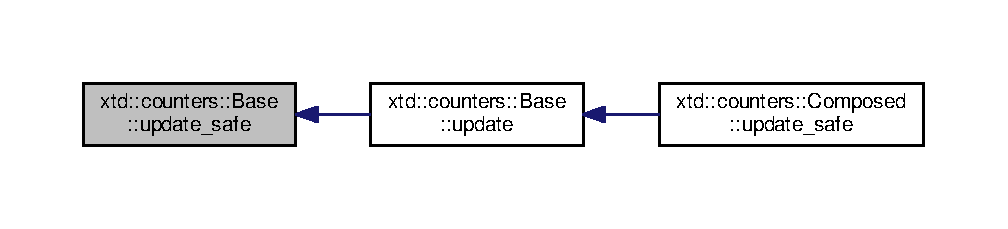
\includegraphics[width=350pt]{classxtd_1_1counters_1_1Base_a8b3d10c9fb2bea1d240f887bbe4008ea_icgraph}
\end{center}
\end{figure}


\index{xtd\+::counters\+::\+Base@{xtd\+::counters\+::\+Base}!visit@{visit}}
\index{visit@{visit}!xtd\+::counters\+::\+Base@{xtd\+::counters\+::\+Base}}
\subsubsection[{\texorpdfstring{visit(\+Visitor \&p\+\_\+visitor) const }{visit(Visitor &p_visitor) const }}]{\setlength{\rightskip}{0pt plus 5cm}void xtd\+::counters\+::\+Base\+::visit (
\begin{DoxyParamCaption}
\item[{{\bf Visitor} \&}]{p\+\_\+visitor}
\end{DoxyParamCaption}
) const}\hypertarget{classxtd_1_1counters_1_1Base_a0c743f0686dc24bada97c2ed31238c02}{}\label{classxtd_1_1counters_1_1Base_a0c743f0686dc24bada97c2ed31238c02}


Definition at line 18 of file Base.\+cc.


\begin{DoxyCode}
19 \{
20   boost::mutex::scoped\_lock l\_lock(\hyperlink{classxtd_1_1counters_1_1Base_aeeac2ffcae02eb6341418d708188a353}{m\_mutex});
21   \hyperlink{classxtd_1_1counters_1_1Base_a0b8f3bdc6880dc03da750aa815dfdf0b}{visit\_safe}(p\_visitor);
22 \}
\end{DoxyCode}


Here is the call graph for this function\+:
\nopagebreak
\begin{figure}[H]
\begin{center}
\leavevmode
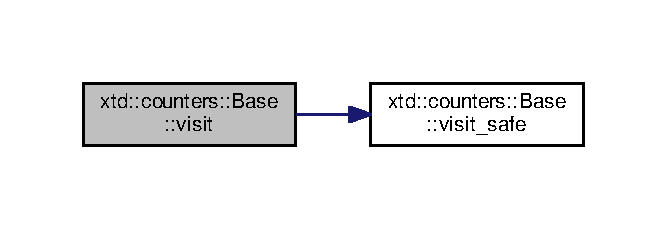
\includegraphics[width=320pt]{classxtd_1_1counters_1_1Base_a0c743f0686dc24bada97c2ed31238c02_cgraph}
\end{center}
\end{figure}




Here is the caller graph for this function\+:
\nopagebreak
\begin{figure}[H]
\begin{center}
\leavevmode
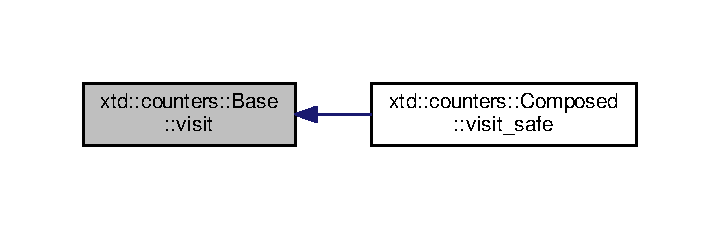
\includegraphics[width=350pt]{classxtd_1_1counters_1_1Base_a0c743f0686dc24bada97c2ed31238c02_icgraph}
\end{center}
\end{figure}


\index{xtd\+::counters\+::\+Base@{xtd\+::counters\+::\+Base}!visit\+\_\+safe@{visit\+\_\+safe}}
\index{visit\+\_\+safe@{visit\+\_\+safe}!xtd\+::counters\+::\+Base@{xtd\+::counters\+::\+Base}}
\subsubsection[{\texorpdfstring{visit\+\_\+safe(\+Visitor \&p\+\_\+visitor) const =0}{visit_safe(Visitor &p_visitor) const =0}}]{\setlength{\rightskip}{0pt plus 5cm}virtual void xtd\+::counters\+::\+Base\+::visit\+\_\+safe (
\begin{DoxyParamCaption}
\item[{{\bf Visitor} \&}]{p\+\_\+visitor}
\end{DoxyParamCaption}
) const\hspace{0.3cm}{\ttfamily [protected]}, {\ttfamily [pure virtual]}}\hypertarget{classxtd_1_1counters_1_1Base_a0b8f3bdc6880dc03da750aa815dfdf0b}{}\label{classxtd_1_1counters_1_1Base_a0b8f3bdc6880dc03da750aa815dfdf0b}


Implemented in \hyperlink{classxtd_1_1counters_1_1Value_a7be35e9a5a52891c5946425152b4db30}{xtd\+::counters\+::\+Value$<$ T\+Type $>$}, \hyperlink{classxtd_1_1counters_1_1Value_a7be35e9a5a52891c5946425152b4db30}{xtd\+::counters\+::\+Value$<$ uint32\+\_\+t $>$}, \hyperlink{classxtd_1_1counters_1_1Composed_a0ef35ed872c3c19d29e2ecc3fa524474}{xtd\+::counters\+::\+Composed}, and \hyperlink{classxtd_1_1counters_1_1ExtValue_af9ea755a42e20d03d325edfe27e05a75}{xtd\+::counters\+::\+Ext\+Value$<$ T\+Type $>$}.



Here is the caller graph for this function\+:
\nopagebreak
\begin{figure}[H]
\begin{center}
\leavevmode
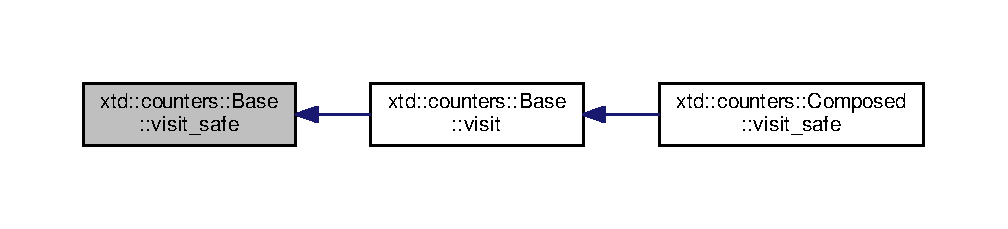
\includegraphics[width=350pt]{classxtd_1_1counters_1_1Base_a0b8f3bdc6880dc03da750aa815dfdf0b_icgraph}
\end{center}
\end{figure}




\subsection{Friends And Related Function Documentation}
\index{xtd\+::counters\+::\+Base@{xtd\+::counters\+::\+Base}!Composed@{Composed}}
\index{Composed@{Composed}!xtd\+::counters\+::\+Base@{xtd\+::counters\+::\+Base}}
\subsubsection[{\texorpdfstring{Composed}{Composed}}]{\setlength{\rightskip}{0pt plus 5cm}friend class {\bf Composed}\hspace{0.3cm}{\ttfamily [friend]}}\hypertarget{classxtd_1_1counters_1_1Base_a93e934ad70d5b32b14beed5572450abf}{}\label{classxtd_1_1counters_1_1Base_a93e934ad70d5b32b14beed5572450abf}


Definition at line 15 of file Base.\+hh.



\subsection{Member Data Documentation}
\index{xtd\+::counters\+::\+Base@{xtd\+::counters\+::\+Base}!m\+\_\+mutex@{m\+\_\+mutex}}
\index{m\+\_\+mutex@{m\+\_\+mutex}!xtd\+::counters\+::\+Base@{xtd\+::counters\+::\+Base}}
\subsubsection[{\texorpdfstring{m\+\_\+mutex}{m_mutex}}]{\setlength{\rightskip}{0pt plus 5cm}boost\+::mutex xtd\+::counters\+::\+Base\+::m\+\_\+mutex\hspace{0.3cm}{\ttfamily [mutable]}, {\ttfamily [protected]}}\hypertarget{classxtd_1_1counters_1_1Base_aeeac2ffcae02eb6341418d708188a353}{}\label{classxtd_1_1counters_1_1Base_aeeac2ffcae02eb6341418d708188a353}


Definition at line 36 of file Base.\+hh.

\index{xtd\+::counters\+::\+Base@{xtd\+::counters\+::\+Base}!m\+\_\+name@{m\+\_\+name}}
\index{m\+\_\+name@{m\+\_\+name}!xtd\+::counters\+::\+Base@{xtd\+::counters\+::\+Base}}
\subsubsection[{\texorpdfstring{m\+\_\+name}{m_name}}]{\setlength{\rightskip}{0pt plus 5cm}string xtd\+::counters\+::\+Base\+::m\+\_\+name\hspace{0.3cm}{\ttfamily [protected]}}\hypertarget{classxtd_1_1counters_1_1Base_ab07d4a6071bfa8263b24d5992bca6960}{}\label{classxtd_1_1counters_1_1Base_ab07d4a6071bfa8263b24d5992bca6960}


Definition at line 35 of file Base.\+hh.



The documentation for this class was generated from the following files\+:\begin{DoxyCompactItemize}
\item 
/home/psyco/dev/xtdcpp/counters/src/\hyperlink{Base_8hh}{Base.\+hh}\item 
/home/psyco/dev/xtdcpp/counters/src/\hyperlink{Base_8cc}{Base.\+cc}\end{DoxyCompactItemize}

\hypertarget{classxtd_1_1counters_1_1Cache}{\section{xtd\-:\-:counters\-:\-:Cache Class Reference}
\label{classxtd_1_1counters_1_1Cache}\index{xtd\-::counters\-::\-Cache@{xtd\-::counters\-::\-Cache}}
}


{\ttfamily \#include $<$Cache.\-hh$>$}



Inheritance diagram for xtd\-:\-:counters\-:\-:Cache\-:
\nopagebreak
\begin{figure}[H]
\begin{center}
\leavevmode
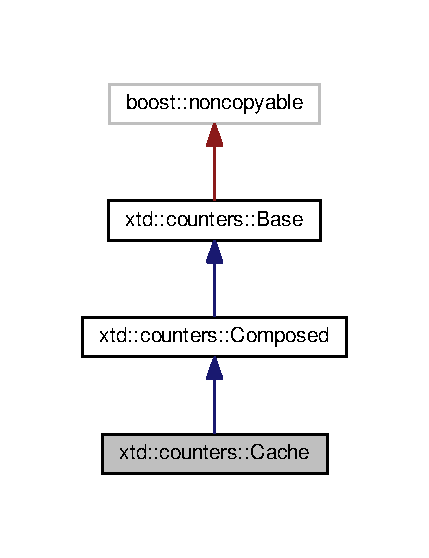
\includegraphics[width=206pt]{classxtd_1_1counters_1_1Cache__inherit__graph}
\end{center}
\end{figure}


Collaboration diagram for xtd\-:\-:counters\-:\-:Cache\-:
\nopagebreak
\begin{figure}[H]
\begin{center}
\leavevmode
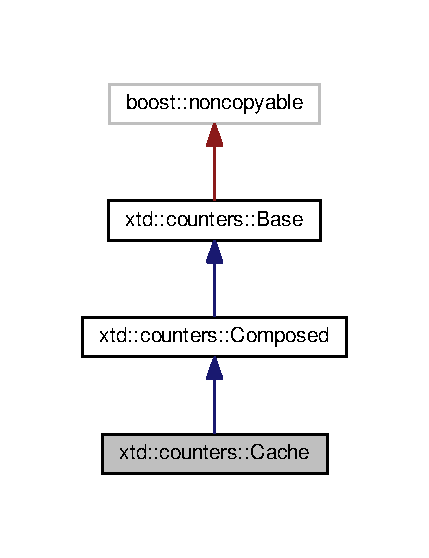
\includegraphics[width=206pt]{classxtd_1_1counters_1_1Cache__coll__graph}
\end{center}
\end{figure}
\subsection*{Public Types}
\begin{DoxyCompactItemize}
\item 
typedef boost\-::shared\-\_\-ptr$<$ \hyperlink{classxtd_1_1counters_1_1Cache}{Cache} $>$ \hyperlink{classxtd_1_1counters_1_1Cache_ad248c57507dbfd4b90332551fd0d5f1b}{t\-\_\-sptr}
\end{DoxyCompactItemize}
\subsection*{Public Member Functions}
\begin{DoxyCompactItemize}
\item 
\hyperlink{classxtd_1_1counters_1_1Cache_a73df8a43eff5fd364e41dccabc562d54}{Cache} (const string \&p\-\_\-name, uint32\-\_\-t p\-\_\-delta\-Time\-Ms=10000)
\item 
void \hyperlink{classxtd_1_1counters_1_1Cache_a57101c273f95f2cf4d5a71627f0b23de}{hit} (void)
\item 
void \hyperlink{classxtd_1_1counters_1_1Cache_a71c25293724fa534633e6d5c9f2cc36d}{miss} (void)
\item 
void \hyperlink{classxtd_1_1counters_1_1Cache_a419b5620c93818158193cb6aca015c9b}{invalid} (void)
\item 
void \hyperlink{classxtd_1_1counters_1_1Cache_a42ea3f207a0399b1864f3ee918e8a0e4}{valid} (void)
\item 
void \hyperlink{classxtd_1_1counters_1_1Cache_a827a66e44b127d38c5f808fa38a2535a}{filtered} (void)
\end{DoxyCompactItemize}
\subsection*{Friends}
\begin{DoxyCompactItemize}
\item 
class \hyperlink{classxtd_1_1counters_1_1Cache_a93e934ad70d5b32b14beed5572450abf}{Composed}
\end{DoxyCompactItemize}
\subsection*{Additional Inherited Members}


\subsection{Detailed Description}
On choisi l'heritage plutot que la composition pour garder une coherence sur la visibilite des methodes internes collect\-\_\-safe update\-\_\-safe (qu'on serait onbligé de mettre en public ou en friend pour faire de la composition). 

Definition at line 22 of file Cache.\-hh.



\subsection{Member Typedef Documentation}
\hypertarget{classxtd_1_1counters_1_1Cache_ad248c57507dbfd4b90332551fd0d5f1b}{\index{xtd\-::counters\-::\-Cache@{xtd\-::counters\-::\-Cache}!t\-\_\-sptr@{t\-\_\-sptr}}
\index{t\-\_\-sptr@{t\-\_\-sptr}!xtd::counters::Cache@{xtd\-::counters\-::\-Cache}}
\subsubsection[{t\-\_\-sptr}]{\setlength{\rightskip}{0pt plus 5cm}typedef boost\-::shared\-\_\-ptr$<${\bf Cache}$>$ {\bf xtd\-::counters\-::\-Cache\-::t\-\_\-sptr}}}\label{classxtd_1_1counters_1_1Cache_ad248c57507dbfd4b90332551fd0d5f1b}


Definition at line 27 of file Cache.\-hh.



\subsection{Constructor \& Destructor Documentation}
\hypertarget{classxtd_1_1counters_1_1Cache_a73df8a43eff5fd364e41dccabc562d54}{\index{xtd\-::counters\-::\-Cache@{xtd\-::counters\-::\-Cache}!Cache@{Cache}}
\index{Cache@{Cache}!xtd::counters::Cache@{xtd\-::counters\-::\-Cache}}
\subsubsection[{Cache}]{\setlength{\rightskip}{0pt plus 5cm}xtd\-::counters\-::\-Cache\-::\-Cache (
\begin{DoxyParamCaption}
\item[{const string \&}]{p\-\_\-name, }
\item[{uint32\-\_\-t}]{p\-\_\-delta\-Time\-Ms = {\ttfamily 10000}}
\end{DoxyParamCaption}
)}}\label{classxtd_1_1counters_1_1Cache_a73df8a43eff5fd364e41dccabc562d54}


Definition at line 9 of file Cache.\-cc.


\begin{DoxyCode}
10                                             :
11   \hyperlink{classxtd_1_1counters_1_1Cache_a93e934ad70d5b32b14beed5572450abf}{Composed}(p\_name),
12   m\_nb                   (\textcolor{stringliteral}{"requests"}),
13   m\_nbFiltered           (\textcolor{stringliteral}{"requests.filtered"}),
14   m\_nbAccepted           (\textcolor{stringliteral}{"requests.accepted"}),
15   m\_nbAcceptedMiss       (\textcolor{stringliteral}{"requests.accepted.miss"}),
16   m\_nbAcceptedHit        (\textcolor{stringliteral}{"requests.accepted.hit"}),
17   m\_nbAcceptedHitInvalid (\textcolor{stringliteral}{"requests.accepted.hit.invalid"}),
18   m\_nbAcceptedHitValid   (\textcolor{stringliteral}{"requests.accepted.hit.valid"}),
19   m\_freqHit              (\textcolor{stringliteral}{"perf.hit"}),
20   m\_freqMiss             (\textcolor{stringliteral}{"perf.miss"}),
21   m\_iFreqHit             (\textcolor{stringliteral}{"perf.instant.hit"}, p\_deltaTimeMs),
22   m\_iFreqMiss            (\textcolor{stringliteral}{"perf.instant.miss"}, p\_deltaTimeMs)
23 \{
24   m\_nb                   = 0;
25   m\_nbFiltered           = 0;
26   m\_nbAccepted           = 0;
27   m\_nbAcceptedMiss       = 0;
28   m\_nbAcceptedHit        = 0;
29   m\_nbAcceptedHitInvalid = 0;
30   m\_nbAcceptedHitValid   = 0;
31 
32   m\_freqMiss    = 0;
33   m\_freqHit     = 0;
34   m\_iFreqMiss   = 0;
35   m\_iFreqHit    = 0;
36 
37   \hyperlink{classxtd_1_1counters_1_1Composed_ac2efbce59510b352a2d47b3118e0d02a}{addItem}(m\_nb);
38   \hyperlink{classxtd_1_1counters_1_1Composed_ac2efbce59510b352a2d47b3118e0d02a}{addItem}(m\_nbFiltered);
39   \hyperlink{classxtd_1_1counters_1_1Composed_ac2efbce59510b352a2d47b3118e0d02a}{addItem}(m\_nbAccepted);
40   \hyperlink{classxtd_1_1counters_1_1Composed_ac2efbce59510b352a2d47b3118e0d02a}{addItem}(m\_nbAcceptedMiss);
41   \hyperlink{classxtd_1_1counters_1_1Composed_ac2efbce59510b352a2d47b3118e0d02a}{addItem}(m\_nbAcceptedHit);
42   \hyperlink{classxtd_1_1counters_1_1Composed_ac2efbce59510b352a2d47b3118e0d02a}{addItem}(m\_nbAcceptedHitInvalid);
43   \hyperlink{classxtd_1_1counters_1_1Composed_ac2efbce59510b352a2d47b3118e0d02a}{addItem}(m\_nbAcceptedHitValid);
44   \hyperlink{classxtd_1_1counters_1_1Composed_ac2efbce59510b352a2d47b3118e0d02a}{addItem}(m\_freqMiss);
45   \hyperlink{classxtd_1_1counters_1_1Composed_ac2efbce59510b352a2d47b3118e0d02a}{addItem}(m\_freqHit);
46   \hyperlink{classxtd_1_1counters_1_1Composed_ac2efbce59510b352a2d47b3118e0d02a}{addItem}(m\_iFreqMiss);
47   \hyperlink{classxtd_1_1counters_1_1Composed_ac2efbce59510b352a2d47b3118e0d02a}{addItem}(m\_iFreqHit);
48 \}
\end{DoxyCode}


Here is the call graph for this function\-:
\nopagebreak
\begin{figure}[H]
\begin{center}
\leavevmode
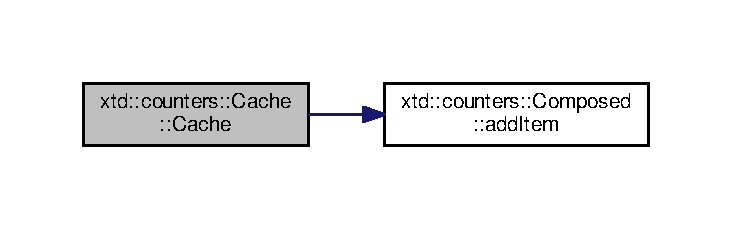
\includegraphics[width=350pt]{classxtd_1_1counters_1_1Cache_a73df8a43eff5fd364e41dccabc562d54_cgraph}
\end{center}
\end{figure}




\subsection{Member Function Documentation}
\hypertarget{classxtd_1_1counters_1_1Cache_a827a66e44b127d38c5f808fa38a2535a}{\index{xtd\-::counters\-::\-Cache@{xtd\-::counters\-::\-Cache}!filtered@{filtered}}
\index{filtered@{filtered}!xtd::counters::Cache@{xtd\-::counters\-::\-Cache}}
\subsubsection[{filtered}]{\setlength{\rightskip}{0pt plus 5cm}void xtd\-::counters\-::\-Cache\-::filtered (
\begin{DoxyParamCaption}
\item[{void}]{}
\end{DoxyParamCaption}
)}}\label{classxtd_1_1counters_1_1Cache_a827a66e44b127d38c5f808fa38a2535a}


Definition at line 83 of file Cache.\-cc.


\begin{DoxyCode}
84 \{
85   m\_nb++;
86   m\_nbFiltered++;
87 \}
\end{DoxyCode}
\hypertarget{classxtd_1_1counters_1_1Cache_a57101c273f95f2cf4d5a71627f0b23de}{\index{xtd\-::counters\-::\-Cache@{xtd\-::counters\-::\-Cache}!hit@{hit}}
\index{hit@{hit}!xtd::counters::Cache@{xtd\-::counters\-::\-Cache}}
\subsubsection[{hit}]{\setlength{\rightskip}{0pt plus 5cm}void xtd\-::counters\-::\-Cache\-::hit (
\begin{DoxyParamCaption}
\item[{void}]{}
\end{DoxyParamCaption}
)}}\label{classxtd_1_1counters_1_1Cache_a57101c273f95f2cf4d5a71627f0b23de}


Definition at line 51 of file Cache.\-cc.


\begin{DoxyCode}
52 \{
53   m\_nb++;
54   m\_nbAccepted++;
55   m\_nbAcceptedHit++;
56   m\_freqHit.\hyperlink{classxtd_1_1counters_1_1Freq_a9e91ea45fc5e9874dc81ca4bd723efc6}{tick}();
57   m\_iFreqHit.\hyperlink{classxtd_1_1counters_1_1InstantFreq_a1760f09b25b97545169be189bf99d250}{tick}();
58 \}
\end{DoxyCode}


Here is the call graph for this function\-:
\nopagebreak
\begin{figure}[H]
\begin{center}
\leavevmode
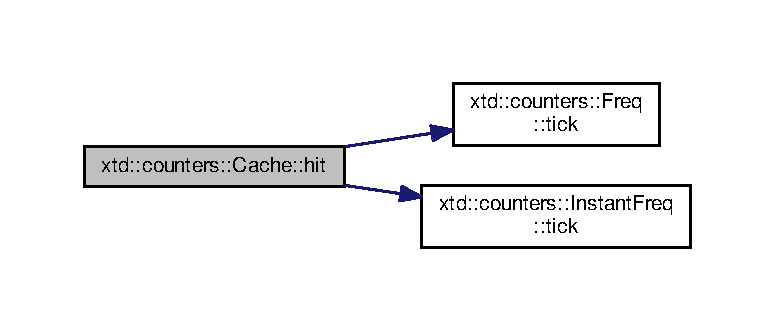
\includegraphics[width=350pt]{classxtd_1_1counters_1_1Cache_a57101c273f95f2cf4d5a71627f0b23de_cgraph}
\end{center}
\end{figure}


\hypertarget{classxtd_1_1counters_1_1Cache_a419b5620c93818158193cb6aca015c9b}{\index{xtd\-::counters\-::\-Cache@{xtd\-::counters\-::\-Cache}!invalid@{invalid}}
\index{invalid@{invalid}!xtd::counters::Cache@{xtd\-::counters\-::\-Cache}}
\subsubsection[{invalid}]{\setlength{\rightskip}{0pt plus 5cm}void xtd\-::counters\-::\-Cache\-::invalid (
\begin{DoxyParamCaption}
\item[{void}]{}
\end{DoxyParamCaption}
)}}\label{classxtd_1_1counters_1_1Cache_a419b5620c93818158193cb6aca015c9b}


Definition at line 71 of file Cache.\-cc.


\begin{DoxyCode}
72 \{
73   m\_nbAcceptedHitInvalid++;
74 \}
\end{DoxyCode}
\hypertarget{classxtd_1_1counters_1_1Cache_a71c25293724fa534633e6d5c9f2cc36d}{\index{xtd\-::counters\-::\-Cache@{xtd\-::counters\-::\-Cache}!miss@{miss}}
\index{miss@{miss}!xtd::counters::Cache@{xtd\-::counters\-::\-Cache}}
\subsubsection[{miss}]{\setlength{\rightskip}{0pt plus 5cm}void xtd\-::counters\-::\-Cache\-::miss (
\begin{DoxyParamCaption}
\item[{void}]{}
\end{DoxyParamCaption}
)}}\label{classxtd_1_1counters_1_1Cache_a71c25293724fa534633e6d5c9f2cc36d}


Definition at line 61 of file Cache.\-cc.


\begin{DoxyCode}
62 \{
63   m\_nb++;
64   m\_nbAccepted++;
65   m\_nbAcceptedMiss++;
66   m\_freqMiss.\hyperlink{classxtd_1_1counters_1_1Freq_a9e91ea45fc5e9874dc81ca4bd723efc6}{tick}();
67   m\_iFreqMiss.\hyperlink{classxtd_1_1counters_1_1InstantFreq_a1760f09b25b97545169be189bf99d250}{tick}();
68 \}
\end{DoxyCode}


Here is the call graph for this function\-:
\nopagebreak
\begin{figure}[H]
\begin{center}
\leavevmode
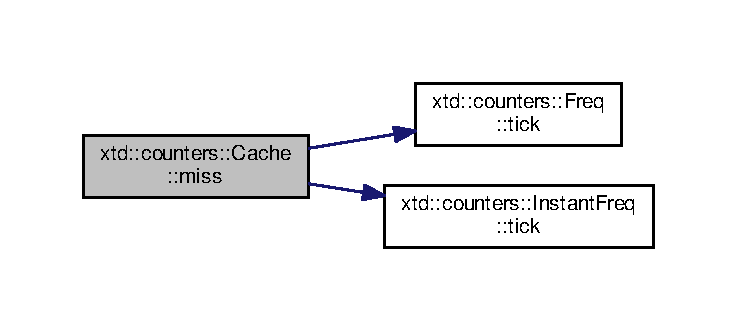
\includegraphics[width=350pt]{classxtd_1_1counters_1_1Cache_a71c25293724fa534633e6d5c9f2cc36d_cgraph}
\end{center}
\end{figure}


\hypertarget{classxtd_1_1counters_1_1Cache_a42ea3f207a0399b1864f3ee918e8a0e4}{\index{xtd\-::counters\-::\-Cache@{xtd\-::counters\-::\-Cache}!valid@{valid}}
\index{valid@{valid}!xtd::counters::Cache@{xtd\-::counters\-::\-Cache}}
\subsubsection[{valid}]{\setlength{\rightskip}{0pt plus 5cm}void xtd\-::counters\-::\-Cache\-::valid (
\begin{DoxyParamCaption}
\item[{void}]{}
\end{DoxyParamCaption}
)}}\label{classxtd_1_1counters_1_1Cache_a42ea3f207a0399b1864f3ee918e8a0e4}


Definition at line 77 of file Cache.\-cc.


\begin{DoxyCode}
78 \{
79   m\_nbAcceptedHitValid++;
80 \}
\end{DoxyCode}


\subsection{Friends And Related Function Documentation}
\hypertarget{classxtd_1_1counters_1_1Cache_a93e934ad70d5b32b14beed5572450abf}{\index{xtd\-::counters\-::\-Cache@{xtd\-::counters\-::\-Cache}!Composed@{Composed}}
\index{Composed@{Composed}!xtd::counters::Cache@{xtd\-::counters\-::\-Cache}}
\subsubsection[{Composed}]{\setlength{\rightskip}{0pt plus 5cm}friend class {\bf Composed}\hspace{0.3cm}{\ttfamily [friend]}}}\label{classxtd_1_1counters_1_1Cache_a93e934ad70d5b32b14beed5572450abf}


Definition at line 24 of file Cache.\-hh.



The documentation for this class was generated from the following files\-:\begin{DoxyCompactItemize}
\item 
/home/travis/build/psycofdj/xtdcpp/counters/src/\hyperlink{Cache_8hh}{Cache.\-hh}\item 
/home/travis/build/psycofdj/xtdcpp/counters/src/\hyperlink{Cache_8cc}{Cache.\-cc}\end{DoxyCompactItemize}

\hypertarget{classxtd_1_1counters_1_1Composed}{}\section{xtd\+:\+:counters\+:\+:Composed Class Reference}
\label{classxtd_1_1counters_1_1Composed}\index{xtd\+::counters\+::\+Composed@{xtd\+::counters\+::\+Composed}}


{\ttfamily \#include $<$Composed.\+hh$>$}



Inheritance diagram for xtd\+:\+:counters\+:\+:Composed\+:
\nopagebreak
\begin{figure}[H]
\begin{center}
\leavevmode
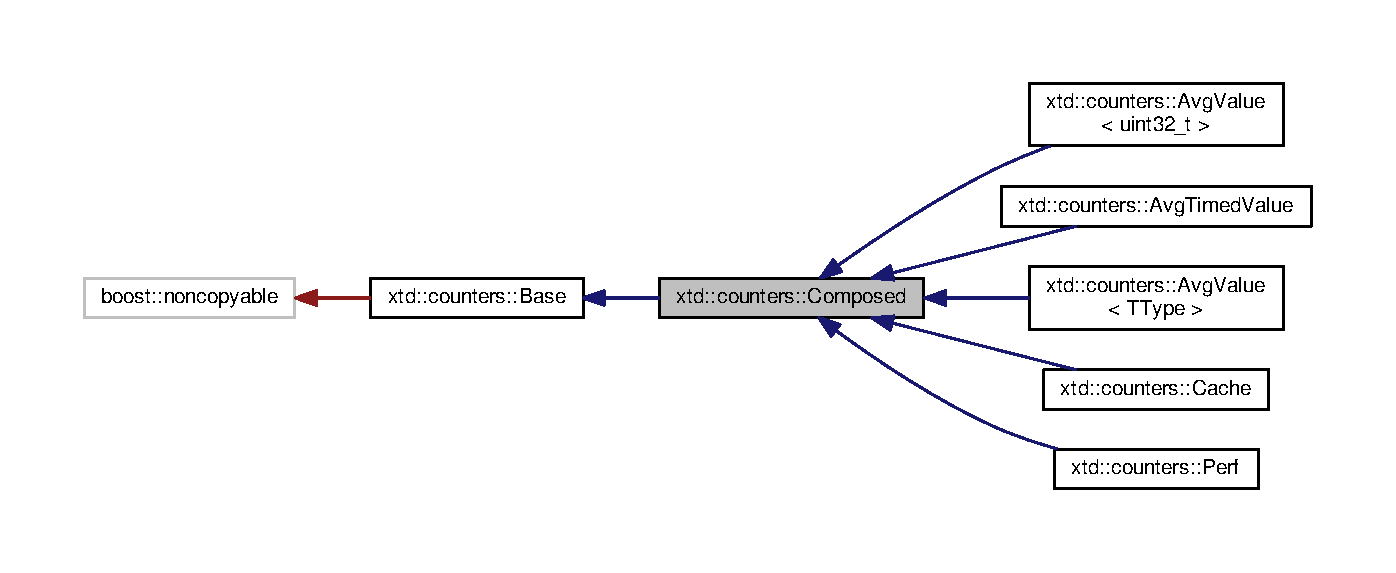
\includegraphics[width=350pt]{classxtd_1_1counters_1_1Composed__inherit__graph}
\end{center}
\end{figure}


Collaboration diagram for xtd\+:\+:counters\+:\+:Composed\+:
\nopagebreak
\begin{figure}[H]
\begin{center}
\leavevmode
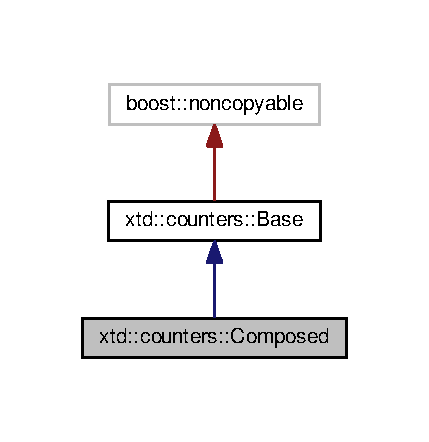
\includegraphics[width=207pt]{classxtd_1_1counters_1_1Composed__coll__graph}
\end{center}
\end{figure}
\subsection*{Public Member Functions}
\begin{DoxyCompactItemize}
\item 
\hyperlink{classxtd_1_1counters_1_1Composed_ad604f1fcd711f6df3c0bca1f07956fe8}{Composed} (const string \&p\+\_\+name)
\item 
virtual \hyperlink{classxtd_1_1counters_1_1Composed_a28b2cf984f727ae3278464e06b03fad7}{$\sim$\+Composed} (void)
\end{DoxyCompactItemize}
\subsection*{Protected Member Functions}
\begin{DoxyCompactItemize}
\item 
void \hyperlink{classxtd_1_1counters_1_1Composed_ac2efbce59510b352a2d47b3118e0d02a}{add\+Item} (\hyperlink{classxtd_1_1counters_1_1Base}{Base} \&p\+\_\+item)
\item 
virtual void \hyperlink{classxtd_1_1counters_1_1Composed_ab6c13e603340cd00da4edc968d747c4d}{update\+\_\+safe} (void)
\item 
virtual void \hyperlink{classxtd_1_1counters_1_1Composed_a0ef35ed872c3c19d29e2ecc3fa524474}{visit\+\_\+safe} (\hyperlink{classxtd_1_1counters_1_1Visitor}{Visitor} \&p\+\_\+visitor) const 
\end{DoxyCompactItemize}
\subsection*{Additional Inherited Members}


\subsection{Detailed Description}


Definition at line 12 of file Composed.\+hh.



\subsection{Constructor \& Destructor Documentation}
\index{xtd\+::counters\+::\+Composed@{xtd\+::counters\+::\+Composed}!Composed@{Composed}}
\index{Composed@{Composed}!xtd\+::counters\+::\+Composed@{xtd\+::counters\+::\+Composed}}
\subsubsection[{\texorpdfstring{Composed(const string \&p\+\_\+name)}{Composed(const string &p_name)}}]{\setlength{\rightskip}{0pt plus 5cm}xtd\+::counters\+::\+Composed\+::\+Composed (
\begin{DoxyParamCaption}
\item[{const string \&}]{p\+\_\+name}
\end{DoxyParamCaption}
)}\hypertarget{classxtd_1_1counters_1_1Composed_ad604f1fcd711f6df3c0bca1f07956fe8}{}\label{classxtd_1_1counters_1_1Composed_ad604f1fcd711f6df3c0bca1f07956fe8}


Definition at line 9 of file Composed.\+cc.


\begin{DoxyCode}
9                                        :
10   \hyperlink{classxtd_1_1counters_1_1Base_ab370a97f3a40bd529e871daedfce60c7}{Base}(p\_name)
11 \{
12 \}
\end{DoxyCode}
\index{xtd\+::counters\+::\+Composed@{xtd\+::counters\+::\+Composed}!````~Composed@{$\sim$\+Composed}}
\index{````~Composed@{$\sim$\+Composed}!xtd\+::counters\+::\+Composed@{xtd\+::counters\+::\+Composed}}
\subsubsection[{\texorpdfstring{$\sim$\+Composed(void)}{~Composed(void)}}]{\setlength{\rightskip}{0pt plus 5cm}virtual xtd\+::counters\+::\+Composed\+::$\sim$\+Composed (
\begin{DoxyParamCaption}
\item[{void}]{}
\end{DoxyParamCaption}
)\hspace{0.3cm}{\ttfamily [inline]}, {\ttfamily [virtual]}}\hypertarget{classxtd_1_1counters_1_1Composed_a28b2cf984f727ae3278464e06b03fad7}{}\label{classxtd_1_1counters_1_1Composed_a28b2cf984f727ae3278464e06b03fad7}


Definition at line 16 of file Composed.\+hh.


\begin{DoxyCode}
16 \{\}
\end{DoxyCode}


Here is the call graph for this function\+:
\nopagebreak
\begin{figure}[H]
\begin{center}
\leavevmode
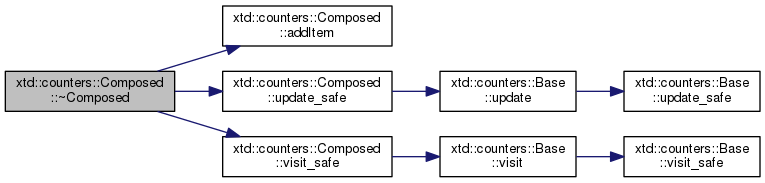
\includegraphics[width=350pt]{classxtd_1_1counters_1_1Composed_a28b2cf984f727ae3278464e06b03fad7_cgraph}
\end{center}
\end{figure}




\subsection{Member Function Documentation}
\index{xtd\+::counters\+::\+Composed@{xtd\+::counters\+::\+Composed}!add\+Item@{add\+Item}}
\index{add\+Item@{add\+Item}!xtd\+::counters\+::\+Composed@{xtd\+::counters\+::\+Composed}}
\subsubsection[{\texorpdfstring{add\+Item(\+Base \&p\+\_\+item)}{addItem(Base &p_item)}}]{\setlength{\rightskip}{0pt plus 5cm}void xtd\+::counters\+::\+Composed\+::add\+Item (
\begin{DoxyParamCaption}
\item[{{\bf Base} \&}]{p\+\_\+item}
\end{DoxyParamCaption}
)\hspace{0.3cm}{\ttfamily [protected]}}\hypertarget{classxtd_1_1counters_1_1Composed_ac2efbce59510b352a2d47b3118e0d02a}{}\label{classxtd_1_1counters_1_1Composed_ac2efbce59510b352a2d47b3118e0d02a}


Definition at line 15 of file Composed.\+cc.


\begin{DoxyCode}
16 \{
17   \textcolor{keywordflow}{if} (0 != \hyperlink{classxtd_1_1counters_1_1Base_ab07d4a6071bfa8263b24d5992bca6960}{m\_name}.size())
18     p\_item.m\_name = \hyperlink{classxtd_1_1counters_1_1Base_ab07d4a6071bfa8263b24d5992bca6960}{m\_name} + \textcolor{stringliteral}{"."} + p\_item.m\_name;
19   m\_items.push\_back(&p\_item);
20 \}
\end{DoxyCode}


Here is the caller graph for this function\+:
\nopagebreak
\begin{figure}[H]
\begin{center}
\leavevmode
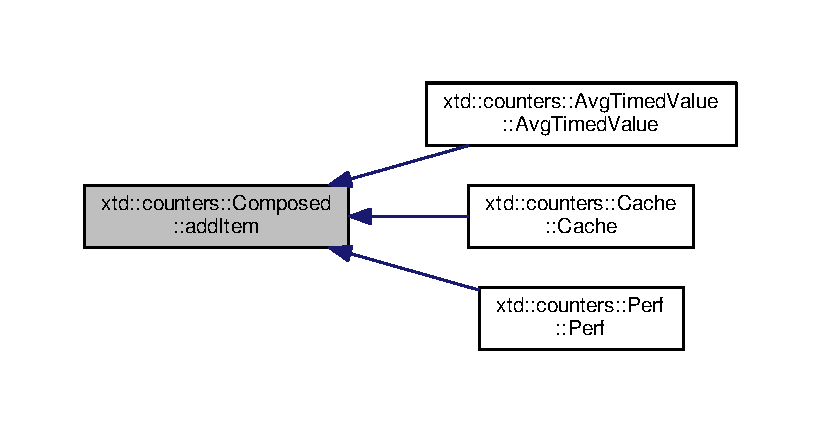
\includegraphics[width=350pt]{classxtd_1_1counters_1_1Composed_ac2efbce59510b352a2d47b3118e0d02a_icgraph}
\end{center}
\end{figure}


\index{xtd\+::counters\+::\+Composed@{xtd\+::counters\+::\+Composed}!update\+\_\+safe@{update\+\_\+safe}}
\index{update\+\_\+safe@{update\+\_\+safe}!xtd\+::counters\+::\+Composed@{xtd\+::counters\+::\+Composed}}
\subsubsection[{\texorpdfstring{update\+\_\+safe(void)}{update_safe(void)}}]{\setlength{\rightskip}{0pt plus 5cm}void xtd\+::counters\+::\+Composed\+::update\+\_\+safe (
\begin{DoxyParamCaption}
\item[{void}]{}
\end{DoxyParamCaption}
)\hspace{0.3cm}{\ttfamily [protected]}, {\ttfamily [virtual]}}\hypertarget{classxtd_1_1counters_1_1Composed_ab6c13e603340cd00da4edc968d747c4d}{}\label{classxtd_1_1counters_1_1Composed_ab6c13e603340cd00da4edc968d747c4d}


Reimplemented from \hyperlink{classxtd_1_1counters_1_1Base_a8b3d10c9fb2bea1d240f887bbe4008ea}{xtd\+::counters\+::\+Base}.



Reimplemented in \hyperlink{classxtd_1_1counters_1_1AvgTimedValue_a1430fd5ff91e960a251b0656c2b5c0ca}{xtd\+::counters\+::\+Avg\+Timed\+Value}.



Definition at line 29 of file Composed.\+cc.


\begin{DoxyCode}
30 \{
31   boost::for\_each(m\_items, boost::bind(&\hyperlink{classxtd_1_1counters_1_1Base_a5ba0d495403ba1ca4e1c6c30d8038dad}{Base::update}, \_1));
32 \}
\end{DoxyCode}


Here is the call graph for this function\+:
\nopagebreak
\begin{figure}[H]
\begin{center}
\leavevmode
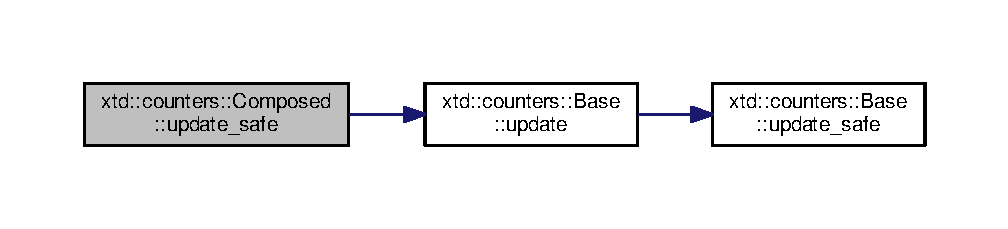
\includegraphics[width=350pt]{classxtd_1_1counters_1_1Composed_ab6c13e603340cd00da4edc968d747c4d_cgraph}
\end{center}
\end{figure}




Here is the caller graph for this function\+:
\nopagebreak
\begin{figure}[H]
\begin{center}
\leavevmode
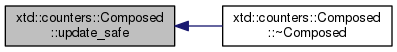
\includegraphics[width=350pt]{classxtd_1_1counters_1_1Composed_ab6c13e603340cd00da4edc968d747c4d_icgraph}
\end{center}
\end{figure}


\index{xtd\+::counters\+::\+Composed@{xtd\+::counters\+::\+Composed}!visit\+\_\+safe@{visit\+\_\+safe}}
\index{visit\+\_\+safe@{visit\+\_\+safe}!xtd\+::counters\+::\+Composed@{xtd\+::counters\+::\+Composed}}
\subsubsection[{\texorpdfstring{visit\+\_\+safe(\+Visitor \&p\+\_\+visitor) const }{visit_safe(Visitor &p_visitor) const }}]{\setlength{\rightskip}{0pt plus 5cm}void xtd\+::counters\+::\+Composed\+::visit\+\_\+safe (
\begin{DoxyParamCaption}
\item[{{\bf Visitor} \&}]{p\+\_\+visitor}
\end{DoxyParamCaption}
) const\hspace{0.3cm}{\ttfamily [protected]}, {\ttfamily [virtual]}}\hypertarget{classxtd_1_1counters_1_1Composed_a0ef35ed872c3c19d29e2ecc3fa524474}{}\label{classxtd_1_1counters_1_1Composed_a0ef35ed872c3c19d29e2ecc3fa524474}


Implements \hyperlink{classxtd_1_1counters_1_1Base_a0b8f3bdc6880dc03da750aa815dfdf0b}{xtd\+::counters\+::\+Base}.



Definition at line 23 of file Composed.\+cc.


\begin{DoxyCode}
24 \{
25   boost::for\_each(m\_items, boost::bind(&\hyperlink{classxtd_1_1counters_1_1Base_a0c743f0686dc24bada97c2ed31238c02}{Base::visit}, \_1, boost::ref(p\_visitor)));
26 \}
\end{DoxyCode}


Here is the call graph for this function\+:
\nopagebreak
\begin{figure}[H]
\begin{center}
\leavevmode
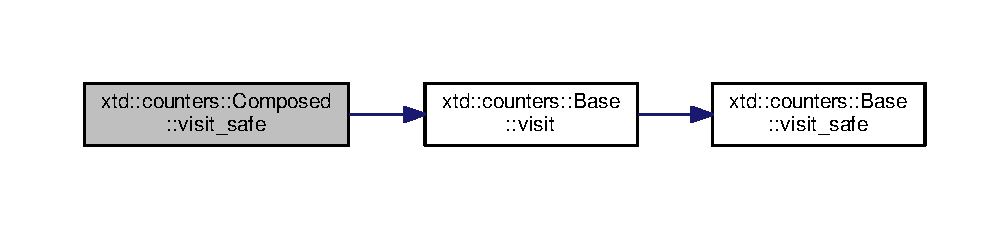
\includegraphics[width=350pt]{classxtd_1_1counters_1_1Composed_a0ef35ed872c3c19d29e2ecc3fa524474_cgraph}
\end{center}
\end{figure}




Here is the caller graph for this function\+:
\nopagebreak
\begin{figure}[H]
\begin{center}
\leavevmode
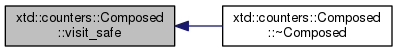
\includegraphics[width=350pt]{classxtd_1_1counters_1_1Composed_a0ef35ed872c3c19d29e2ecc3fa524474_icgraph}
\end{center}
\end{figure}




The documentation for this class was generated from the following files\+:\begin{DoxyCompactItemize}
\item 
/home/psyco/dev/xtdcpp/counters/src/\hyperlink{Composed_8hh}{Composed.\+hh}\item 
/home/psyco/dev/xtdcpp/counters/src/\hyperlink{Composed_8cc}{Composed.\+cc}\end{DoxyCompactItemize}

\hypertarget{classxtd_1_1counters_1_1CounterManager}{}\section{xtd\+:\+:counters\+:\+:Counter\+Manager Class Reference}
\label{classxtd_1_1counters_1_1CounterManager}\index{xtd\+::counters\+::\+Counter\+Manager@{xtd\+::counters\+::\+Counter\+Manager}}


{\ttfamily \#include $<$Counter\+Manager.\+hh$>$}

\subsection*{Public Types}
\begin{DoxyCompactItemize}
\item 
typedef boost\+::shared\+\_\+ptr$<$ \hyperlink{classxtd_1_1counters_1_1CounterManager}{Counter\+Manager} $>$ \hyperlink{classxtd_1_1counters_1_1CounterManager_ac136b7de8a55b55a2700d93901ba1e9a}{t\+\_\+sptr}
\item 
typedef std\+::multimap$<$ boost\+::filesystem\+::path, \hyperlink{classxtd_1_1counters_1_1Base_aa0ea634f1a5e3df87418566a3e8fcbd6}{Base\+::t\+\_\+sptr} $>$ \hyperlink{classxtd_1_1counters_1_1CounterManager_ae675635fccfde42cc3831d07adacd2cb}{t\+\_\+counters}
\end{DoxyCompactItemize}
\subsection*{Public Member Functions}
\begin{DoxyCompactItemize}
\item 
\hyperlink{classxtd_1_1counters_1_1CounterManager_a13c765c1d8c326d3a040c779975d0149}{Counter\+Manager} (const uint32\+\_\+t p\+\_\+deplay, const string \&p\+\_\+path)
\item 
virtual \hyperlink{classxtd_1_1counters_1_1CounterManager_aff5438182c449dd719382d2d8ca2b1c8}{$\sim$\+Counter\+Manager} (void)
\item 
status \hyperlink{classxtd_1_1counters_1_1CounterManager_a65755963d9293fa457c6562a38b2dff3}{start} (void)
\item 
void \hyperlink{classxtd_1_1counters_1_1CounterManager_a2b50e714f748fc2298bd3ca0c77c668d}{stop} (void)
\item 
void \hyperlink{classxtd_1_1counters_1_1CounterManager_a1677a12619a23ba162a19ebc74fe41e9}{to\+Json} (boost\+::property\+\_\+tree\+::ptree \&p\+\_\+dst)
\item 
string \hyperlink{classxtd_1_1counters_1_1CounterManager_a01f164d28b794064ed5cba2ab94e3583}{get\+Snmp\+Path} (void) const 
\item 
status \hyperlink{classxtd_1_1counters_1_1CounterManager_a7e0f54fa25b0d8592362159604cc4310}{add} (\hyperlink{classxtd_1_1counters_1_1Base_aa0ea634f1a5e3df87418566a3e8fcbd6}{Base\+::t\+\_\+sptr} p\+\_\+counter, const string \&p\+\_\+path)
\item 
const \hyperlink{classxtd_1_1counters_1_1CounterManager_ae675635fccfde42cc3831d07adacd2cb}{t\+\_\+counters} \hyperlink{classxtd_1_1counters_1_1CounterManager_afb314857888b269ca3ea0f2b4870b3e5}{get\+Counters} (void)
\item 
void \hyperlink{classxtd_1_1counters_1_1CounterManager_a6b9bb7cbdc06c137d04d7a944232b264}{write\+On\+Disk} (void) const 
\end{DoxyCompactItemize}


\subsection{Detailed Description}


Definition at line 18 of file Counter\+Manager.\+hh.



\subsection{Member Typedef Documentation}
\index{xtd\+::counters\+::\+Counter\+Manager@{xtd\+::counters\+::\+Counter\+Manager}!t\+\_\+counters@{t\+\_\+counters}}
\index{t\+\_\+counters@{t\+\_\+counters}!xtd\+::counters\+::\+Counter\+Manager@{xtd\+::counters\+::\+Counter\+Manager}}
\subsubsection[{\texorpdfstring{t\+\_\+counters}{t_counters}}]{\setlength{\rightskip}{0pt plus 5cm}typedef std\+::multimap$<$boost\+::filesystem\+::path, {\bf Base\+::t\+\_\+sptr}$>$ {\bf xtd\+::counters\+::\+Counter\+Manager\+::t\+\_\+counters}}\hypertarget{classxtd_1_1counters_1_1CounterManager_ae675635fccfde42cc3831d07adacd2cb}{}\label{classxtd_1_1counters_1_1CounterManager_ae675635fccfde42cc3831d07adacd2cb}


Definition at line 23 of file Counter\+Manager.\+hh.

\index{xtd\+::counters\+::\+Counter\+Manager@{xtd\+::counters\+::\+Counter\+Manager}!t\+\_\+sptr@{t\+\_\+sptr}}
\index{t\+\_\+sptr@{t\+\_\+sptr}!xtd\+::counters\+::\+Counter\+Manager@{xtd\+::counters\+::\+Counter\+Manager}}
\subsubsection[{\texorpdfstring{t\+\_\+sptr}{t_sptr}}]{\setlength{\rightskip}{0pt plus 5cm}typedef boost\+::shared\+\_\+ptr$<${\bf Counter\+Manager}$>$ {\bf xtd\+::counters\+::\+Counter\+Manager\+::t\+\_\+sptr}}\hypertarget{classxtd_1_1counters_1_1CounterManager_ac136b7de8a55b55a2700d93901ba1e9a}{}\label{classxtd_1_1counters_1_1CounterManager_ac136b7de8a55b55a2700d93901ba1e9a}


Definition at line 22 of file Counter\+Manager.\+hh.



\subsection{Constructor \& Destructor Documentation}
\index{xtd\+::counters\+::\+Counter\+Manager@{xtd\+::counters\+::\+Counter\+Manager}!Counter\+Manager@{Counter\+Manager}}
\index{Counter\+Manager@{Counter\+Manager}!xtd\+::counters\+::\+Counter\+Manager@{xtd\+::counters\+::\+Counter\+Manager}}
\subsubsection[{\texorpdfstring{Counter\+Manager(const uint32\+\_\+t p\+\_\+deplay, const string \&p\+\_\+path)}{CounterManager(const uint32_t p_deplay, const string &p_path)}}]{\setlength{\rightskip}{0pt plus 5cm}xtd\+::counters\+::\+Counter\+Manager\+::\+Counter\+Manager (
\begin{DoxyParamCaption}
\item[{const uint32\+\_\+t}]{p\+\_\+deplay, }
\item[{const string \&}]{p\+\_\+path}
\end{DoxyParamCaption}
)}\hypertarget{classxtd_1_1counters_1_1CounterManager_a13c765c1d8c326d3a040c779975d0149}{}\label{classxtd_1_1counters_1_1CounterManager_a13c765c1d8c326d3a040c779975d0149}


Definition at line 21 of file Counter\+Manager.\+cc.


\begin{DoxyCode}
21                                                                            :
22   m\_refreshDelay(p\_delay),
23   m\_snmpPath(p\_path),
24   m\_counters(),
25   m\_isRunning(\textcolor{keyword}{false})
26 \{
27 \}
\end{DoxyCode}
\index{xtd\+::counters\+::\+Counter\+Manager@{xtd\+::counters\+::\+Counter\+Manager}!````~Counter\+Manager@{$\sim$\+Counter\+Manager}}
\index{````~Counter\+Manager@{$\sim$\+Counter\+Manager}!xtd\+::counters\+::\+Counter\+Manager@{xtd\+::counters\+::\+Counter\+Manager}}
\subsubsection[{\texorpdfstring{$\sim$\+Counter\+Manager(void)}{~CounterManager(void)}}]{\setlength{\rightskip}{0pt plus 5cm}xtd\+::counters\+::\+Counter\+Manager\+::$\sim$\+Counter\+Manager (
\begin{DoxyParamCaption}
\item[{void}]{}
\end{DoxyParamCaption}
)\hspace{0.3cm}{\ttfamily [virtual]}}\hypertarget{classxtd_1_1counters_1_1CounterManager_aff5438182c449dd719382d2d8ca2b1c8}{}\label{classxtd_1_1counters_1_1CounterManager_aff5438182c449dd719382d2d8ca2b1c8}


Definition at line 29 of file Counter\+Manager.\+cc.


\begin{DoxyCode}
30 \{
31 \}
\end{DoxyCode}


\subsection{Member Function Documentation}
\index{xtd\+::counters\+::\+Counter\+Manager@{xtd\+::counters\+::\+Counter\+Manager}!add@{add}}
\index{add@{add}!xtd\+::counters\+::\+Counter\+Manager@{xtd\+::counters\+::\+Counter\+Manager}}
\subsubsection[{\texorpdfstring{add(\+Base\+::t\+\_\+sptr p\+\_\+counter, const string \&p\+\_\+path)}{add(Base::t_sptr p_counter, const string &p_path)}}]{\setlength{\rightskip}{0pt plus 5cm}status xtd\+::counters\+::\+Counter\+Manager\+::add (
\begin{DoxyParamCaption}
\item[{{\bf Base\+::t\+\_\+sptr}}]{p\+\_\+counter, }
\item[{const string \&}]{p\+\_\+path}
\end{DoxyParamCaption}
)}\hypertarget{classxtd_1_1counters_1_1CounterManager_a7e0f54fa25b0d8592362159604cc4310}{}\label{classxtd_1_1counters_1_1CounterManager_a7e0f54fa25b0d8592362159604cc4310}


Definition at line 69 of file Counter\+Manager.\+cc.


\begin{DoxyCode}
70 \{
71   bfs::path l\_subDir(p\_subDir);
72   m\_counters.insert(std::make\_pair(l\_subDir, p\_counter));
73   \textcolor{keywordflow}{return} \hyperlink{namespacextd_1_1counters_a408a8b2fd75b44228e1741ac4a32aff8a444bcb3a3fcf8389296c49467f27e1d6}{status::ok};
74 \}
\end{DoxyCode}
\index{xtd\+::counters\+::\+Counter\+Manager@{xtd\+::counters\+::\+Counter\+Manager}!get\+Counters@{get\+Counters}}
\index{get\+Counters@{get\+Counters}!xtd\+::counters\+::\+Counter\+Manager@{xtd\+::counters\+::\+Counter\+Manager}}
\subsubsection[{\texorpdfstring{get\+Counters(void)}{getCounters(void)}}]{\setlength{\rightskip}{0pt plus 5cm}const {\bf Counter\+Manager\+::t\+\_\+counters} xtd\+::counters\+::\+Counter\+Manager\+::get\+Counters (
\begin{DoxyParamCaption}
\item[{void}]{}
\end{DoxyParamCaption}
)}\hypertarget{classxtd_1_1counters_1_1CounterManager_afb314857888b269ca3ea0f2b4870b3e5}{}\label{classxtd_1_1counters_1_1CounterManager_afb314857888b269ca3ea0f2b4870b3e5}


Definition at line 63 of file Counter\+Manager.\+cc.


\begin{DoxyCode}
64 \{
65   \textcolor{keywordflow}{return} m\_counters;
66 \}
\end{DoxyCode}
\index{xtd\+::counters\+::\+Counter\+Manager@{xtd\+::counters\+::\+Counter\+Manager}!get\+Snmp\+Path@{get\+Snmp\+Path}}
\index{get\+Snmp\+Path@{get\+Snmp\+Path}!xtd\+::counters\+::\+Counter\+Manager@{xtd\+::counters\+::\+Counter\+Manager}}
\subsubsection[{\texorpdfstring{get\+Snmp\+Path(void) const }{getSnmpPath(void) const }}]{\setlength{\rightskip}{0pt plus 5cm}string xtd\+::counters\+::\+Counter\+Manager\+::get\+Snmp\+Path (
\begin{DoxyParamCaption}
\item[{void}]{}
\end{DoxyParamCaption}
) const}\hypertarget{classxtd_1_1counters_1_1CounterManager_a01f164d28b794064ed5cba2ab94e3583}{}\label{classxtd_1_1counters_1_1CounterManager_a01f164d28b794064ed5cba2ab94e3583}


Definition at line 57 of file Counter\+Manager.\+cc.


\begin{DoxyCode}
58 \{
59   \textcolor{keywordflow}{return} m\_snmpPath;
60 \}
\end{DoxyCode}
\index{xtd\+::counters\+::\+Counter\+Manager@{xtd\+::counters\+::\+Counter\+Manager}!start@{start}}
\index{start@{start}!xtd\+::counters\+::\+Counter\+Manager@{xtd\+::counters\+::\+Counter\+Manager}}
\subsubsection[{\texorpdfstring{start(void)}{start(void)}}]{\setlength{\rightskip}{0pt plus 5cm}status xtd\+::counters\+::\+Counter\+Manager\+::start (
\begin{DoxyParamCaption}
\item[{void}]{}
\end{DoxyParamCaption}
)}\hypertarget{classxtd_1_1counters_1_1CounterManager_a65755963d9293fa457c6562a38b2dff3}{}\label{classxtd_1_1counters_1_1CounterManager_a65755963d9293fa457c6562a38b2dff3}


Definition at line 34 of file Counter\+Manager.\+cc.


\begin{DoxyCode}
35 \{
36   \textcolor{keywordflow}{if} (m\_counters.size() == 0)
37   \{
38     logger::crit(\textcolor{stringliteral}{"counters.manager"}, \textcolor{stringliteral}{"no counter to monitor"}, HERE);
39     \textcolor{keywordflow}{return} \hyperlink{namespacextd_1_1counters_a408a8b2fd75b44228e1741ac4a32aff8acb5e100e5a9a3e7f6d1fd97512215282}{status::error};
40   \}
41 
42   t\_counters::const\_iterator l\_it = m\_counters.begin();
43 
44   \textcolor{keywordflow}{for} (; l\_it != m\_counters.end(); l\_it++)
45   \{
46     \textcolor{keywordtype}{string} l\_path = m\_snmpPath + \textcolor{stringliteral}{"/"} + (*l\_it).first.string() + \textcolor{stringliteral}{"/"};
47     bfs::create\_directories(l\_path);
48   \}
49 
50   m\_isRunning = \textcolor{keyword}{true};
51   m\_thread    = boost::thread(boost::bind(&CounterManager::refresh, \textcolor{keyword}{this}));
52 
53   \textcolor{keywordflow}{return} \hyperlink{namespacextd_1_1counters_a408a8b2fd75b44228e1741ac4a32aff8a444bcb3a3fcf8389296c49467f27e1d6}{status::ok};
54 \}
\end{DoxyCode}
\index{xtd\+::counters\+::\+Counter\+Manager@{xtd\+::counters\+::\+Counter\+Manager}!stop@{stop}}
\index{stop@{stop}!xtd\+::counters\+::\+Counter\+Manager@{xtd\+::counters\+::\+Counter\+Manager}}
\subsubsection[{\texorpdfstring{stop(void)}{stop(void)}}]{\setlength{\rightskip}{0pt plus 5cm}void xtd\+::counters\+::\+Counter\+Manager\+::stop (
\begin{DoxyParamCaption}
\item[{void}]{}
\end{DoxyParamCaption}
)}\hypertarget{classxtd_1_1counters_1_1CounterManager_a2b50e714f748fc2298bd3ca0c77c668d}{}\label{classxtd_1_1counters_1_1CounterManager_a2b50e714f748fc2298bd3ca0c77c668d}


Definition at line 77 of file Counter\+Manager.\+cc.


\begin{DoxyCode}
78 \{
79   \textcolor{keywordflow}{if} (m\_isRunning)
80   \{
81     m\_isRunning = \textcolor{keyword}{false};
82     m\_thread.interrupt();
83     m\_thread.join();
84     \hyperlink{classxtd_1_1counters_1_1CounterManager_a6b9bb7cbdc06c137d04d7a944232b264}{writeOnDisk}();
85   \}
86 \}
\end{DoxyCode}


Here is the call graph for this function\+:
\nopagebreak
\begin{figure}[H]
\begin{center}
\leavevmode
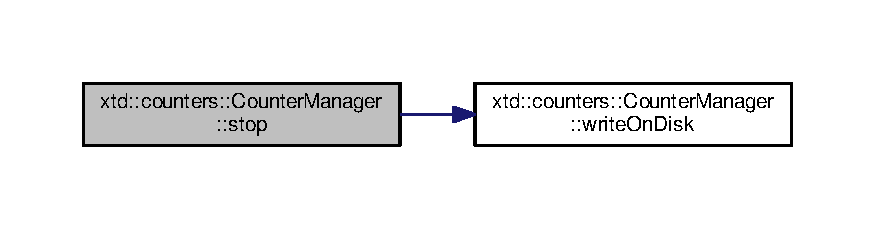
\includegraphics[width=350pt]{classxtd_1_1counters_1_1CounterManager_a2b50e714f748fc2298bd3ca0c77c668d_cgraph}
\end{center}
\end{figure}


\index{xtd\+::counters\+::\+Counter\+Manager@{xtd\+::counters\+::\+Counter\+Manager}!to\+Json@{to\+Json}}
\index{to\+Json@{to\+Json}!xtd\+::counters\+::\+Counter\+Manager@{xtd\+::counters\+::\+Counter\+Manager}}
\subsubsection[{\texorpdfstring{to\+Json(boost\+::property\+\_\+tree\+::ptree \&p\+\_\+dst)}{toJson(boost::property_tree::ptree &p_dst)}}]{\setlength{\rightskip}{0pt plus 5cm}void xtd\+::counters\+::\+Counter\+Manager\+::to\+Json (
\begin{DoxyParamCaption}
\item[{boost\+::property\+\_\+tree\+::ptree \&}]{p\+\_\+dst}
\end{DoxyParamCaption}
)}\hypertarget{classxtd_1_1counters_1_1CounterManager_a1677a12619a23ba162a19ebc74fe41e9}{}\label{classxtd_1_1counters_1_1CounterManager_a1677a12619a23ba162a19ebc74fe41e9}


Definition at line 89 of file Counter\+Manager.\+cc.


\begin{DoxyCode}
90 \{
91   \textcolor{keywordtype}{string} l\_path;
92 
93   \textcolor{keywordflow}{for} (\textcolor{keyword}{auto}& c\_data : m\_counters)
94   \{
95     l\_path = c\_data.first.string();
96     boost::replace\_all(l\_path, \textcolor{stringliteral}{"/"}, \textcolor{stringliteral}{"!"});
97 
98     boost::property\_tree::ptree::path\_type l\_jsonPath(l\_path, \textcolor{charliteral}{'!'});
99     JsonVisitor                            l\_jsonVisitor(l\_jsonPath, p\_json);
100     c\_data.second->update();
101     c\_data.second->visit(l\_jsonVisitor);
102   \}
103 \}
\end{DoxyCode}


Here is the call graph for this function\+:
\nopagebreak
\begin{figure}[H]
\begin{center}
\leavevmode
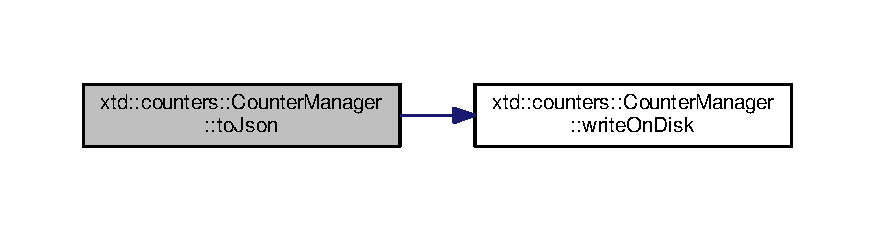
\includegraphics[width=350pt]{classxtd_1_1counters_1_1CounterManager_a1677a12619a23ba162a19ebc74fe41e9_cgraph}
\end{center}
\end{figure}


\index{xtd\+::counters\+::\+Counter\+Manager@{xtd\+::counters\+::\+Counter\+Manager}!write\+On\+Disk@{write\+On\+Disk}}
\index{write\+On\+Disk@{write\+On\+Disk}!xtd\+::counters\+::\+Counter\+Manager@{xtd\+::counters\+::\+Counter\+Manager}}
\subsubsection[{\texorpdfstring{write\+On\+Disk(void) const }{writeOnDisk(void) const }}]{\setlength{\rightskip}{0pt plus 5cm}void xtd\+::counters\+::\+Counter\+Manager\+::write\+On\+Disk (
\begin{DoxyParamCaption}
\item[{void}]{}
\end{DoxyParamCaption}
) const}\hypertarget{classxtd_1_1counters_1_1CounterManager_a6b9bb7cbdc06c137d04d7a944232b264}{}\label{classxtd_1_1counters_1_1CounterManager_a6b9bb7cbdc06c137d04d7a944232b264}


Definition at line 116 of file Counter\+Manager.\+cc.


\begin{DoxyCode}
117 \{
118   \textcolor{keywordflow}{for} (\textcolor{keyword}{auto}& c\_data : m\_counters)
119   \{
120     bfs::path   l\_path(bfs::path(m\_snmpPath) / c\_data.first);
121     FileVisitor l\_fileVisitor(l\_path);
122 
123     c\_data.second->update();
124     c\_data.second->visit(l\_fileVisitor);
125   \}
126 \}
\end{DoxyCode}


Here is the caller graph for this function\+:
\nopagebreak
\begin{figure}[H]
\begin{center}
\leavevmode
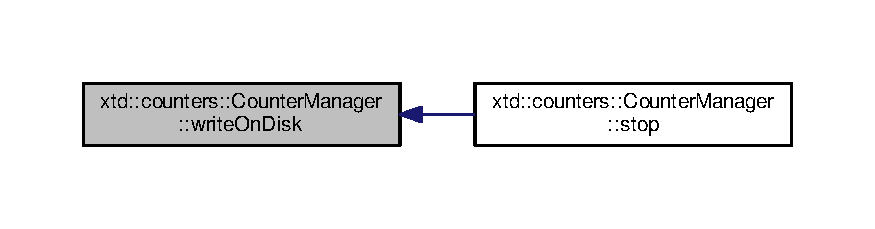
\includegraphics[width=350pt]{classxtd_1_1counters_1_1CounterManager_a6b9bb7cbdc06c137d04d7a944232b264_icgraph}
\end{center}
\end{figure}




The documentation for this class was generated from the following files\+:\begin{DoxyCompactItemize}
\item 
/home/psyco/dev/xtdcpp/counters/src/\hyperlink{CounterManager_8hh}{Counter\+Manager.\+hh}\item 
/home/psyco/dev/xtdcpp/counters/src/\hyperlink{CounterManager_8cc}{Counter\+Manager.\+cc}\end{DoxyCompactItemize}

\hypertarget{classxtd_1_1counters_1_1ExtValue}{\section{xtd\-:\-:counters\-:\-:Ext\-Value$<$ T\-Type $>$ Class Template Reference}
\label{classxtd_1_1counters_1_1ExtValue}\index{xtd\-::counters\-::\-Ext\-Value$<$ T\-Type $>$@{xtd\-::counters\-::\-Ext\-Value$<$ T\-Type $>$}}
}


{\ttfamily \#include $<$counters\-\_\-fwd.\-hh$>$}



Inheritance diagram for xtd\-:\-:counters\-:\-:Ext\-Value$<$ T\-Type $>$\-:
\nopagebreak
\begin{figure}[H]
\begin{center}
\leavevmode
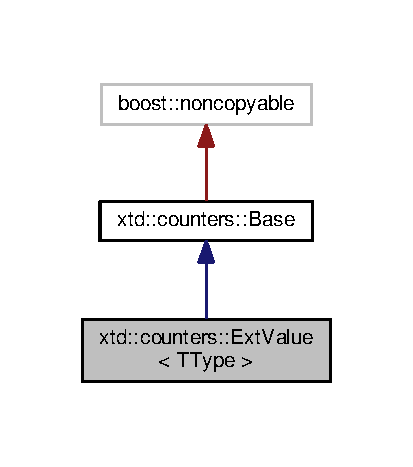
\includegraphics[width=198pt]{classxtd_1_1counters_1_1ExtValue__inherit__graph}
\end{center}
\end{figure}


Collaboration diagram for xtd\-:\-:counters\-:\-:Ext\-Value$<$ T\-Type $>$\-:
\nopagebreak
\begin{figure}[H]
\begin{center}
\leavevmode
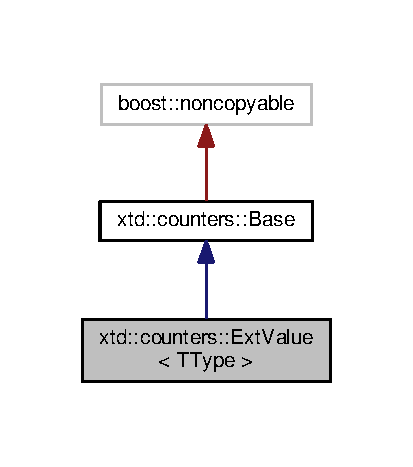
\includegraphics[width=198pt]{classxtd_1_1counters_1_1ExtValue__coll__graph}
\end{center}
\end{figure}
\subsection*{Public Member Functions}
\begin{DoxyCompactItemize}
\item 
\hyperlink{classxtd_1_1counters_1_1ExtValue_ac56f634edb50ac47aca158e479bebeae}{Ext\-Value} (const string \&p\-\_\-name, const T\-Type \&p\-\_\-value)
\item 
virtual \hyperlink{classxtd_1_1counters_1_1ExtValue_a33aa51f76d3abae665265f3cea64a293}{$\sim$\-Ext\-Value} (void)
\end{DoxyCompactItemize}
\subsection*{Protected Member Functions}
\begin{DoxyCompactItemize}
\item 
void \hyperlink{classxtd_1_1counters_1_1ExtValue_af9ea755a42e20d03d325edfe27e05a75}{visit\-\_\-safe} (\hyperlink{classxtd_1_1counters_1_1Visitor}{Visitor} \&p\-\_\-visitor) const 
\end{DoxyCompactItemize}
\subsection*{Friends}
\begin{DoxyCompactItemize}
\item 
class \hyperlink{classxtd_1_1counters_1_1ExtValue_a93e934ad70d5b32b14beed5572450abf}{Composed}
\end{DoxyCompactItemize}
\subsection*{Additional Inherited Members}


\subsection{Detailed Description}
\subsubsection*{template$<$typename T\-Type$>$class xtd\-::counters\-::\-Ext\-Value$<$ T\-Type $>$}



Definition at line 10 of file counters\-\_\-fwd.\-hh.



\subsection{Constructor \& Destructor Documentation}
\hypertarget{classxtd_1_1counters_1_1ExtValue_ac56f634edb50ac47aca158e479bebeae}{\index{xtd\-::counters\-::\-Ext\-Value@{xtd\-::counters\-::\-Ext\-Value}!Ext\-Value@{Ext\-Value}}
\index{Ext\-Value@{Ext\-Value}!xtd::counters::ExtValue@{xtd\-::counters\-::\-Ext\-Value}}
\subsubsection[{Ext\-Value}]{\setlength{\rightskip}{0pt plus 5cm}template$<$typename T\-Type $>$ {\bf xtd\-::counters\-::\-Ext\-Value}$<$ T\-Type $>$\-::{\bf Ext\-Value} (
\begin{DoxyParamCaption}
\item[{const string \&}]{p\-\_\-name, }
\item[{const T\-Type \&}]{p\-\_\-value}
\end{DoxyParamCaption}
)}}\label{classxtd_1_1counters_1_1ExtValue_ac56f634edb50ac47aca158e479bebeae}
\hypertarget{classxtd_1_1counters_1_1ExtValue_a33aa51f76d3abae665265f3cea64a293}{\index{xtd\-::counters\-::\-Ext\-Value@{xtd\-::counters\-::\-Ext\-Value}!$\sim$\-Ext\-Value@{$\sim$\-Ext\-Value}}
\index{$\sim$\-Ext\-Value@{$\sim$\-Ext\-Value}!xtd::counters::ExtValue@{xtd\-::counters\-::\-Ext\-Value}}
\subsubsection[{$\sim$\-Ext\-Value}]{\setlength{\rightskip}{0pt plus 5cm}template$<$typename T\-Type $>$ virtual {\bf xtd\-::counters\-::\-Ext\-Value}$<$ T\-Type $>$\-::$\sim${\bf Ext\-Value} (
\begin{DoxyParamCaption}
\item[{void}]{}
\end{DoxyParamCaption}
)\hspace{0.3cm}{\ttfamily [inline]}, {\ttfamily [virtual]}}}\label{classxtd_1_1counters_1_1ExtValue_a33aa51f76d3abae665265f3cea64a293}


Definition at line 19 of file Ext\-Value.\-hh.


\begin{DoxyCode}
19 \{\};
\end{DoxyCode}


\subsection{Member Function Documentation}
\hypertarget{classxtd_1_1counters_1_1ExtValue_af9ea755a42e20d03d325edfe27e05a75}{\index{xtd\-::counters\-::\-Ext\-Value@{xtd\-::counters\-::\-Ext\-Value}!visit\-\_\-safe@{visit\-\_\-safe}}
\index{visit\-\_\-safe@{visit\-\_\-safe}!xtd::counters::ExtValue@{xtd\-::counters\-::\-Ext\-Value}}
\subsubsection[{visit\-\_\-safe}]{\setlength{\rightskip}{0pt plus 5cm}template$<$typename T\-Type $>$ void {\bf xtd\-::counters\-::\-Ext\-Value}$<$ T\-Type $>$\-::visit\-\_\-safe (
\begin{DoxyParamCaption}
\item[{{\bf Visitor} \&}]{p\-\_\-visitor}
\end{DoxyParamCaption}
) const\hspace{0.3cm}{\ttfamily [protected]}, {\ttfamily [virtual]}}}\label{classxtd_1_1counters_1_1ExtValue_af9ea755a42e20d03d325edfe27e05a75}


Implements \hyperlink{classxtd_1_1counters_1_1Base_a0b8f3bdc6880dc03da750aa815dfdf0b}{xtd\-::counters\-::\-Base}.



\subsection{Friends And Related Function Documentation}
\hypertarget{classxtd_1_1counters_1_1ExtValue_a93e934ad70d5b32b14beed5572450abf}{\index{xtd\-::counters\-::\-Ext\-Value@{xtd\-::counters\-::\-Ext\-Value}!Composed@{Composed}}
\index{Composed@{Composed}!xtd::counters::ExtValue@{xtd\-::counters\-::\-Ext\-Value}}
\subsubsection[{Composed}]{\setlength{\rightskip}{0pt plus 5cm}template$<$typename T\-Type $>$ friend class {\bf Composed}\hspace{0.3cm}{\ttfamily [friend]}}}\label{classxtd_1_1counters_1_1ExtValue_a93e934ad70d5b32b14beed5572450abf}


Definition at line 15 of file Ext\-Value.\-hh.



The documentation for this class was generated from the following files\-:\begin{DoxyCompactItemize}
\item 
/home/travis/build/psycofdj/xtdcpp/counters/src/\hyperlink{counters__fwd_8hh}{counters\-\_\-fwd.\-hh}\item 
/home/travis/build/psycofdj/xtdcpp/counters/src/\hyperlink{ExtValue_8hh}{Ext\-Value.\-hh}\end{DoxyCompactItemize}

\hypertarget{classxtd_1_1counters_1_1FileVisitor}{\section{xtd\-:\-:counters\-:\-:File\-Visitor Class Reference}
\label{classxtd_1_1counters_1_1FileVisitor}\index{xtd\-::counters\-::\-File\-Visitor@{xtd\-::counters\-::\-File\-Visitor}}
}


{\ttfamily \#include $<$File\-Visitor.\-hh$>$}



Inheritance diagram for xtd\-:\-:counters\-:\-:File\-Visitor\-:
\nopagebreak
\begin{figure}[H]
\begin{center}
\leavevmode
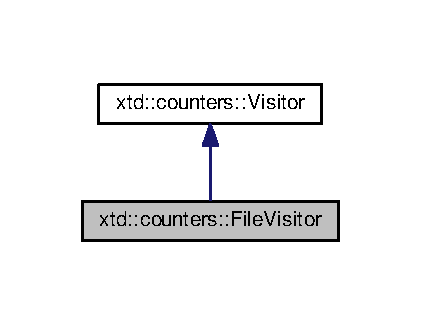
\includegraphics[width=202pt]{classxtd_1_1counters_1_1FileVisitor__inherit__graph}
\end{center}
\end{figure}


Collaboration diagram for xtd\-:\-:counters\-:\-:File\-Visitor\-:
\nopagebreak
\begin{figure}[H]
\begin{center}
\leavevmode
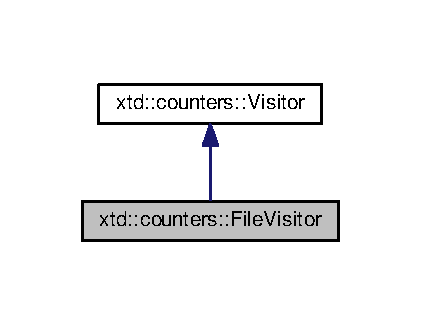
\includegraphics[width=202pt]{classxtd_1_1counters_1_1FileVisitor__coll__graph}
\end{center}
\end{figure}
\subsection*{Public Member Functions}
\begin{DoxyCompactItemize}
\item 
\hyperlink{classxtd_1_1counters_1_1FileVisitor_a1cdf1a2d8abde62c1e4d340e4b68351d}{File\-Visitor} (const t\-\_\-path \&p\-\_\-path)
\item 
void \hyperlink{classxtd_1_1counters_1_1FileVisitor_af6936e3e1e62880b0eb9fc76b0b0a120}{operator()} (const string \&p\-\_\-name, const string \&p\-\_\-data)
\item 
void \hyperlink{classxtd_1_1counters_1_1FileVisitor_a69214d261c695bb48335c58ed2a76cae}{operator()} (const string \&p\-\_\-name, uint8\-\_\-t p\-\_\-data)
\item 
void \hyperlink{classxtd_1_1counters_1_1FileVisitor_a687eff42ec19d5aed86689e0405fa181}{operator()} (const string \&p\-\_\-name, uint16\-\_\-t p\-\_\-data)
\item 
void \hyperlink{classxtd_1_1counters_1_1FileVisitor_ae5807c31711d611b93e435071855ce2f}{operator()} (const string \&p\-\_\-name, uint32\-\_\-t p\-\_\-data)
\item 
void \hyperlink{classxtd_1_1counters_1_1FileVisitor_a9e5edd247355cc9c3387d1bd5cda0642}{operator()} (const string \&p\-\_\-name, uint64\-\_\-t p\-\_\-data)
\end{DoxyCompactItemize}


\subsection{Detailed Description}


Definition at line 14 of file File\-Visitor.\-hh.



\subsection{Constructor \& Destructor Documentation}
\hypertarget{classxtd_1_1counters_1_1FileVisitor_a1cdf1a2d8abde62c1e4d340e4b68351d}{\index{xtd\-::counters\-::\-File\-Visitor@{xtd\-::counters\-::\-File\-Visitor}!File\-Visitor@{File\-Visitor}}
\index{File\-Visitor@{File\-Visitor}!xtd::counters::FileVisitor@{xtd\-::counters\-::\-File\-Visitor}}
\subsubsection[{File\-Visitor}]{\setlength{\rightskip}{0pt plus 5cm}xtd\-::counters\-::\-File\-Visitor\-::\-File\-Visitor (
\begin{DoxyParamCaption}
\item[{const t\-\_\-path \&}]{p\-\_\-path}
\end{DoxyParamCaption}
)\hspace{0.3cm}{\ttfamily [inline]}}}\label{classxtd_1_1counters_1_1FileVisitor_a1cdf1a2d8abde62c1e4d340e4b68351d}


Definition at line 20 of file File\-Visitor.\-hh.


\begin{DoxyCode}
20                                     :
21     m\_path(p\_path)
22   \{
23   \}
\end{DoxyCode}


\subsection{Member Function Documentation}
\hypertarget{classxtd_1_1counters_1_1FileVisitor_af6936e3e1e62880b0eb9fc76b0b0a120}{\index{xtd\-::counters\-::\-File\-Visitor@{xtd\-::counters\-::\-File\-Visitor}!operator()@{operator()}}
\index{operator()@{operator()}!xtd::counters::FileVisitor@{xtd\-::counters\-::\-File\-Visitor}}
\subsubsection[{operator()}]{\setlength{\rightskip}{0pt plus 5cm}void xtd\-::counters\-::\-File\-Visitor\-::operator() (
\begin{DoxyParamCaption}
\item[{const string \&}]{p\-\_\-name, }
\item[{const string \&}]{p\-\_\-data}
\end{DoxyParamCaption}
)\hspace{0.3cm}{\ttfamily [inline]}, {\ttfamily [virtual]}}}\label{classxtd_1_1counters_1_1FileVisitor_af6936e3e1e62880b0eb9fc76b0b0a120}


Implements \hyperlink{classxtd_1_1counters_1_1Visitor_a1341281b8c4cbf4de5a37e035f75e214}{xtd\-::counters\-::\-Visitor}.



Definition at line 26 of file File\-Visitor.\-hh.


\begin{DoxyCode}
26 \{ write(p\_name, p\_data); \}
\end{DoxyCode}
\hypertarget{classxtd_1_1counters_1_1FileVisitor_a69214d261c695bb48335c58ed2a76cae}{\index{xtd\-::counters\-::\-File\-Visitor@{xtd\-::counters\-::\-File\-Visitor}!operator()@{operator()}}
\index{operator()@{operator()}!xtd::counters::FileVisitor@{xtd\-::counters\-::\-File\-Visitor}}
\subsubsection[{operator()}]{\setlength{\rightskip}{0pt plus 5cm}void xtd\-::counters\-::\-File\-Visitor\-::operator() (
\begin{DoxyParamCaption}
\item[{const string \&}]{p\-\_\-name, }
\item[{uint8\-\_\-t}]{p\-\_\-data}
\end{DoxyParamCaption}
)\hspace{0.3cm}{\ttfamily [inline]}, {\ttfamily [virtual]}}}\label{classxtd_1_1counters_1_1FileVisitor_a69214d261c695bb48335c58ed2a76cae}


Implements \hyperlink{classxtd_1_1counters_1_1Visitor_a1a5da2c523703b0c9132595f22e1700e}{xtd\-::counters\-::\-Visitor}.



Definition at line 27 of file File\-Visitor.\-hh.


\begin{DoxyCode}
27 \{ write(p\_name, p\_data); \}
\end{DoxyCode}
\hypertarget{classxtd_1_1counters_1_1FileVisitor_a687eff42ec19d5aed86689e0405fa181}{\index{xtd\-::counters\-::\-File\-Visitor@{xtd\-::counters\-::\-File\-Visitor}!operator()@{operator()}}
\index{operator()@{operator()}!xtd::counters::FileVisitor@{xtd\-::counters\-::\-File\-Visitor}}
\subsubsection[{operator()}]{\setlength{\rightskip}{0pt plus 5cm}void xtd\-::counters\-::\-File\-Visitor\-::operator() (
\begin{DoxyParamCaption}
\item[{const string \&}]{p\-\_\-name, }
\item[{uint16\-\_\-t}]{p\-\_\-data}
\end{DoxyParamCaption}
)\hspace{0.3cm}{\ttfamily [inline]}, {\ttfamily [virtual]}}}\label{classxtd_1_1counters_1_1FileVisitor_a687eff42ec19d5aed86689e0405fa181}


Implements \hyperlink{classxtd_1_1counters_1_1Visitor_a6139d735b720a83e87f49932855f1ade}{xtd\-::counters\-::\-Visitor}.



Definition at line 28 of file File\-Visitor.\-hh.


\begin{DoxyCode}
28 \{ write(p\_name, p\_data); \}
\end{DoxyCode}
\hypertarget{classxtd_1_1counters_1_1FileVisitor_ae5807c31711d611b93e435071855ce2f}{\index{xtd\-::counters\-::\-File\-Visitor@{xtd\-::counters\-::\-File\-Visitor}!operator()@{operator()}}
\index{operator()@{operator()}!xtd::counters::FileVisitor@{xtd\-::counters\-::\-File\-Visitor}}
\subsubsection[{operator()}]{\setlength{\rightskip}{0pt plus 5cm}void xtd\-::counters\-::\-File\-Visitor\-::operator() (
\begin{DoxyParamCaption}
\item[{const string \&}]{p\-\_\-name, }
\item[{uint32\-\_\-t}]{p\-\_\-data}
\end{DoxyParamCaption}
)\hspace{0.3cm}{\ttfamily [inline]}, {\ttfamily [virtual]}}}\label{classxtd_1_1counters_1_1FileVisitor_ae5807c31711d611b93e435071855ce2f}


Implements \hyperlink{classxtd_1_1counters_1_1Visitor_a0bc4c30e3df6ef796878b85ce1be17fb}{xtd\-::counters\-::\-Visitor}.



Definition at line 29 of file File\-Visitor.\-hh.


\begin{DoxyCode}
29 \{ write(p\_name, p\_data); \}
\end{DoxyCode}
\hypertarget{classxtd_1_1counters_1_1FileVisitor_a9e5edd247355cc9c3387d1bd5cda0642}{\index{xtd\-::counters\-::\-File\-Visitor@{xtd\-::counters\-::\-File\-Visitor}!operator()@{operator()}}
\index{operator()@{operator()}!xtd::counters::FileVisitor@{xtd\-::counters\-::\-File\-Visitor}}
\subsubsection[{operator()}]{\setlength{\rightskip}{0pt plus 5cm}void xtd\-::counters\-::\-File\-Visitor\-::operator() (
\begin{DoxyParamCaption}
\item[{const string \&}]{p\-\_\-name, }
\item[{uint64\-\_\-t}]{p\-\_\-data}
\end{DoxyParamCaption}
)\hspace{0.3cm}{\ttfamily [inline]}, {\ttfamily [virtual]}}}\label{classxtd_1_1counters_1_1FileVisitor_a9e5edd247355cc9c3387d1bd5cda0642}


Implements \hyperlink{classxtd_1_1counters_1_1Visitor_aba895c10dd1a28fa7a8b64e61adee5ac}{xtd\-::counters\-::\-Visitor}.



Definition at line 30 of file File\-Visitor.\-hh.


\begin{DoxyCode}
30 \{ write(p\_name, p\_data); \}
\end{DoxyCode}


The documentation for this class was generated from the following file\-:\begin{DoxyCompactItemize}
\item 
/home/travis/build/psycofdj/xtdcpp/counters/src/\hyperlink{FileVisitor_8hh}{File\-Visitor.\-hh}\end{DoxyCompactItemize}

\hypertarget{classxtd_1_1counters_1_1Freq}{}\section{xtd\+:\+:counters\+:\+:Freq Class Reference}
\label{classxtd_1_1counters_1_1Freq}\index{xtd\+::counters\+::\+Freq@{xtd\+::counters\+::\+Freq}}


{\ttfamily \#include $<$Freq.\+hh$>$}



Inheritance diagram for xtd\+:\+:counters\+:\+:Freq\+:
\nopagebreak
\begin{figure}[H]
\begin{center}
\leavevmode
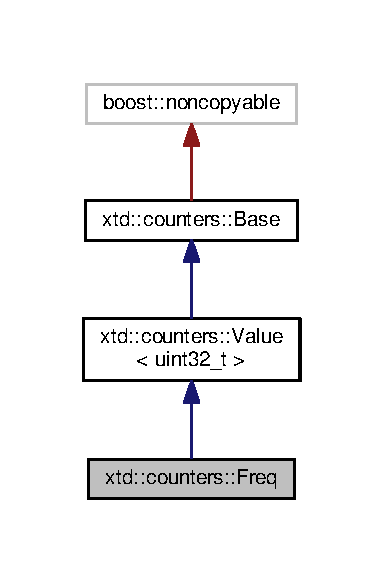
\includegraphics[width=184pt]{classxtd_1_1counters_1_1Freq__inherit__graph}
\end{center}
\end{figure}


Collaboration diagram for xtd\+:\+:counters\+:\+:Freq\+:
\nopagebreak
\begin{figure}[H]
\begin{center}
\leavevmode
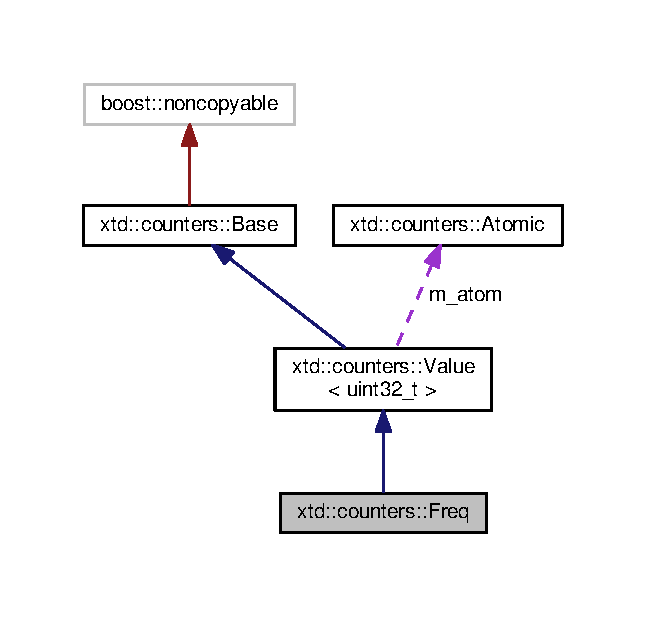
\includegraphics[width=310pt]{classxtd_1_1counters_1_1Freq__coll__graph}
\end{center}
\end{figure}
\subsection*{Public Member Functions}
\begin{DoxyCompactItemize}
\item 
\hyperlink{classxtd_1_1counters_1_1Freq_ac48f859e66bef29a24a2cd9e2ad2aff6}{Freq} (const string \&p\+\_\+name)
\item 
virtual \hyperlink{classxtd_1_1counters_1_1Freq_ac5d39dc4ea5211f48bf6f4834fe2558b}{$\sim$\+Freq} (void)
\item 
void \hyperlink{classxtd_1_1counters_1_1Freq_a9e91ea45fc5e9874dc81ca4bd723efc6}{tick} (void)
\item 
\hyperlink{classxtd_1_1counters_1_1Freq}{Freq} \& \hyperlink{classxtd_1_1counters_1_1Freq_a622e28502b8613bbac6fd40f324ddb8c}{operator=} (const uint32\+\_\+t \&p\+\_\+value)
\end{DoxyCompactItemize}
\subsection*{Protected Member Functions}
\begin{DoxyCompactItemize}
\item 
virtual void \hyperlink{classxtd_1_1counters_1_1Freq_af4ee512e594def96c8bd907d2a369729}{update\+\_\+safe} (void)
\end{DoxyCompactItemize}
\subsection*{Friends}
\begin{DoxyCompactItemize}
\item 
class \hyperlink{classxtd_1_1counters_1_1Freq_a93e934ad70d5b32b14beed5572450abf}{Composed}
\end{DoxyCompactItemize}
\subsection*{Additional Inherited Members}


\subsection{Detailed Description}


Definition at line 11 of file Freq.\+hh.



\subsection{Constructor \& Destructor Documentation}
\index{xtd\+::counters\+::\+Freq@{xtd\+::counters\+::\+Freq}!Freq@{Freq}}
\index{Freq@{Freq}!xtd\+::counters\+::\+Freq@{xtd\+::counters\+::\+Freq}}
\subsubsection[{\texorpdfstring{Freq(const string \&p\+\_\+name)}{Freq(const string &p_name)}}]{\setlength{\rightskip}{0pt plus 5cm}xtd\+::counters\+::\+Freq\+::\+Freq (
\begin{DoxyParamCaption}
\item[{const string \&}]{p\+\_\+name}
\end{DoxyParamCaption}
)}\hypertarget{classxtd_1_1counters_1_1Freq_ac48f859e66bef29a24a2cd9e2ad2aff6}{}\label{classxtd_1_1counters_1_1Freq_ac48f859e66bef29a24a2cd9e2ad2aff6}


Definition at line 14 of file Freq.\+cc.


\begin{DoxyCode}
14                                :
15   \hyperlink{classxtd_1_1counters_1_1Value_a298f146ab57eaed8e6f783c26e78e0f4}{Value}(p\_name),
16   m\_beginTime(bpt::microsec\_clock::local\_time()),
17   m\_nbEvent(0)
18 \{
19 \}
\end{DoxyCode}
\index{xtd\+::counters\+::\+Freq@{xtd\+::counters\+::\+Freq}!````~Freq@{$\sim$\+Freq}}
\index{````~Freq@{$\sim$\+Freq}!xtd\+::counters\+::\+Freq@{xtd\+::counters\+::\+Freq}}
\subsubsection[{\texorpdfstring{$\sim$\+Freq(void)}{~Freq(void)}}]{\setlength{\rightskip}{0pt plus 5cm}virtual xtd\+::counters\+::\+Freq\+::$\sim$\+Freq (
\begin{DoxyParamCaption}
\item[{void}]{}
\end{DoxyParamCaption}
)\hspace{0.3cm}{\ttfamily [inline]}, {\ttfamily [virtual]}}\hypertarget{classxtd_1_1counters_1_1Freq_ac5d39dc4ea5211f48bf6f4834fe2558b}{}\label{classxtd_1_1counters_1_1Freq_ac5d39dc4ea5211f48bf6f4834fe2558b}


Definition at line 17 of file Freq.\+hh.


\begin{DoxyCode}
17 \{\}
\end{DoxyCode}


Here is the call graph for this function\+:
\nopagebreak
\begin{figure}[H]
\begin{center}
\leavevmode
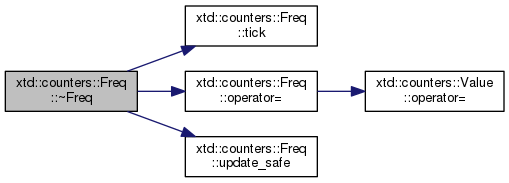
\includegraphics[width=350pt]{classxtd_1_1counters_1_1Freq_ac5d39dc4ea5211f48bf6f4834fe2558b_cgraph}
\end{center}
\end{figure}




\subsection{Member Function Documentation}
\index{xtd\+::counters\+::\+Freq@{xtd\+::counters\+::\+Freq}!operator=@{operator=}}
\index{operator=@{operator=}!xtd\+::counters\+::\+Freq@{xtd\+::counters\+::\+Freq}}
\subsubsection[{\texorpdfstring{operator=(const uint32\+\_\+t \&p\+\_\+value)}{operator=(const uint32_t &p_value)}}]{\setlength{\rightskip}{0pt plus 5cm}{\bf Freq} \& xtd\+::counters\+::\+Freq\+::operator= (
\begin{DoxyParamCaption}
\item[{const uint32\+\_\+t \&}]{p\+\_\+value}
\end{DoxyParamCaption}
)}\hypertarget{classxtd_1_1counters_1_1Freq_a622e28502b8613bbac6fd40f324ddb8c}{}\label{classxtd_1_1counters_1_1Freq_a622e28502b8613bbac6fd40f324ddb8c}


Definition at line 22 of file Freq.\+cc.


\begin{DoxyCode}
23 \{
24   \hyperlink{classxtd_1_1counters_1_1Value_a017667569f4177e0c44836ef4e9bc7b0}{Value<uint32\_t>::operator=}(p\_value);
25   \textcolor{keywordflow}{return} *\textcolor{keyword}{this};
26 \}
\end{DoxyCode}


Here is the call graph for this function\+:
\nopagebreak
\begin{figure}[H]
\begin{center}
\leavevmode
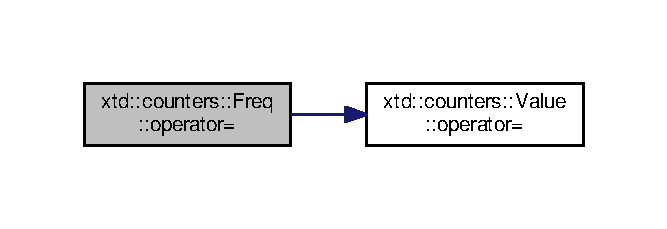
\includegraphics[width=319pt]{classxtd_1_1counters_1_1Freq_a622e28502b8613bbac6fd40f324ddb8c_cgraph}
\end{center}
\end{figure}




Here is the caller graph for this function\+:
\nopagebreak
\begin{figure}[H]
\begin{center}
\leavevmode
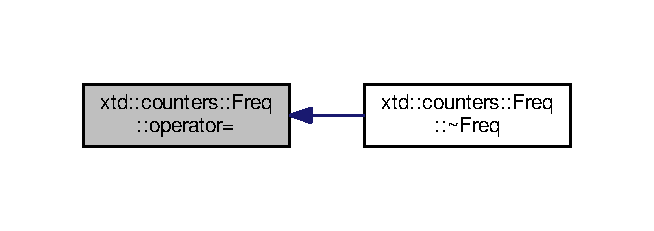
\includegraphics[width=314pt]{classxtd_1_1counters_1_1Freq_a622e28502b8613bbac6fd40f324ddb8c_icgraph}
\end{center}
\end{figure}


\index{xtd\+::counters\+::\+Freq@{xtd\+::counters\+::\+Freq}!tick@{tick}}
\index{tick@{tick}!xtd\+::counters\+::\+Freq@{xtd\+::counters\+::\+Freq}}
\subsubsection[{\texorpdfstring{tick(void)}{tick(void)}}]{\setlength{\rightskip}{0pt plus 5cm}void xtd\+::counters\+::\+Freq\+::tick (
\begin{DoxyParamCaption}
\item[{void}]{}
\end{DoxyParamCaption}
)}\hypertarget{classxtd_1_1counters_1_1Freq_a9e91ea45fc5e9874dc81ca4bd723efc6}{}\label{classxtd_1_1counters_1_1Freq_a9e91ea45fc5e9874dc81ca4bd723efc6}


Definition at line 29 of file Freq.\+cc.


\begin{DoxyCode}
30 \{
31   atom::atomic\_inc32(&m\_nbEvent);
32 \}
\end{DoxyCode}


Here is the caller graph for this function\+:
\nopagebreak
\begin{figure}[H]
\begin{center}
\leavevmode
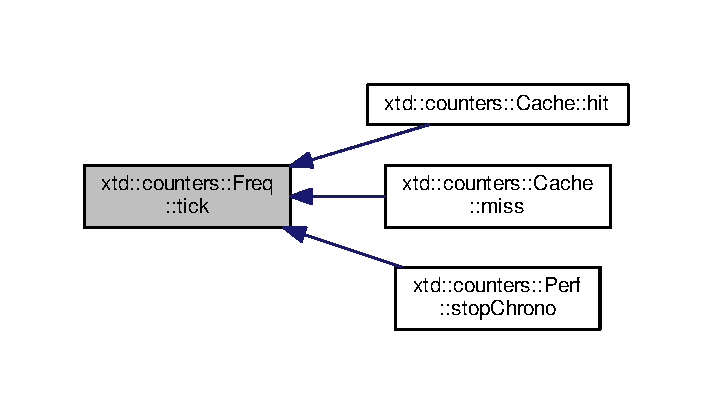
\includegraphics[width=350pt]{classxtd_1_1counters_1_1Freq_a9e91ea45fc5e9874dc81ca4bd723efc6_icgraph}
\end{center}
\end{figure}


\index{xtd\+::counters\+::\+Freq@{xtd\+::counters\+::\+Freq}!update\+\_\+safe@{update\+\_\+safe}}
\index{update\+\_\+safe@{update\+\_\+safe}!xtd\+::counters\+::\+Freq@{xtd\+::counters\+::\+Freq}}
\subsubsection[{\texorpdfstring{update\+\_\+safe(void)}{update_safe(void)}}]{\setlength{\rightskip}{0pt plus 5cm}void xtd\+::counters\+::\+Freq\+::update\+\_\+safe (
\begin{DoxyParamCaption}
\item[{void}]{}
\end{DoxyParamCaption}
)\hspace{0.3cm}{\ttfamily [protected]}, {\ttfamily [virtual]}}\hypertarget{classxtd_1_1counters_1_1Freq_af4ee512e594def96c8bd907d2a369729}{}\label{classxtd_1_1counters_1_1Freq_af4ee512e594def96c8bd907d2a369729}


Reimplemented from \hyperlink{classxtd_1_1counters_1_1Base_a8b3d10c9fb2bea1d240f887bbe4008ea}{xtd\+::counters\+::\+Base}.



Definition at line 36 of file Freq.\+cc.


\begin{DoxyCode}
37 \{
38   bpt::time\_duration l\_diffTime = bpt::microsec\_clock::local\_time() - m\_beginTime;
39 
40   \textcolor{keywordflow}{if} (l\_diffTime.total\_milliseconds() == 0)
41     \textcolor{keywordflow}{return};
42   \hyperlink{classxtd_1_1counters_1_1Value_abe06c1cebededaf2f216707171f63c3c}{m\_value} = (m\_nbEvent * 1000) / l\_diffTime.total\_milliseconds();
43 \}
\end{DoxyCode}


Here is the caller graph for this function\+:
\nopagebreak
\begin{figure}[H]
\begin{center}
\leavevmode
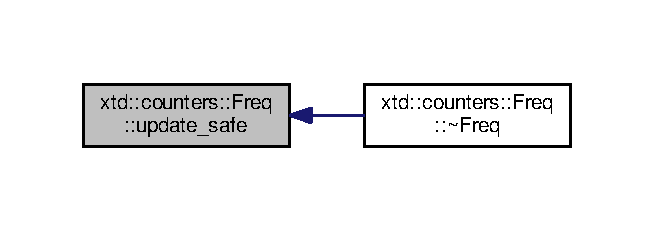
\includegraphics[width=314pt]{classxtd_1_1counters_1_1Freq_af4ee512e594def96c8bd907d2a369729_icgraph}
\end{center}
\end{figure}




\subsection{Friends And Related Function Documentation}
\index{xtd\+::counters\+::\+Freq@{xtd\+::counters\+::\+Freq}!Composed@{Composed}}
\index{Composed@{Composed}!xtd\+::counters\+::\+Freq@{xtd\+::counters\+::\+Freq}}
\subsubsection[{\texorpdfstring{Composed}{Composed}}]{\setlength{\rightskip}{0pt plus 5cm}friend class {\bf Composed}\hspace{0.3cm}{\ttfamily [friend]}}\hypertarget{classxtd_1_1counters_1_1Freq_a93e934ad70d5b32b14beed5572450abf}{}\label{classxtd_1_1counters_1_1Freq_a93e934ad70d5b32b14beed5572450abf}


Definition at line 13 of file Freq.\+hh.



The documentation for this class was generated from the following files\+:\begin{DoxyCompactItemize}
\item 
/home/psyco/dev/xtdcpp/counters/src/\hyperlink{Freq_8hh}{Freq.\+hh}\item 
/home/psyco/dev/xtdcpp/counters/src/\hyperlink{Freq_8cc}{Freq.\+cc}\end{DoxyCompactItemize}

\hypertarget{classxtd_1_1counters_1_1InstantFreq}{\section{xtd\-:\-:counters\-:\-:Instant\-Freq Class Reference}
\label{classxtd_1_1counters_1_1InstantFreq}\index{xtd\-::counters\-::\-Instant\-Freq@{xtd\-::counters\-::\-Instant\-Freq}}
}


{\ttfamily \#include $<$Instant\-Freq.\-hh$>$}



Inheritance diagram for xtd\-:\-:counters\-:\-:Instant\-Freq\-:
\nopagebreak
\begin{figure}[H]
\begin{center}
\leavevmode
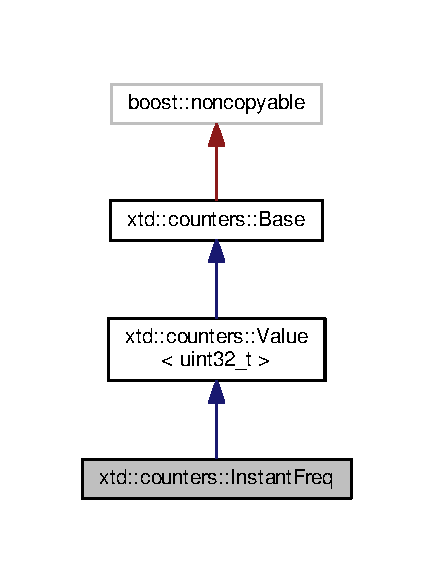
\includegraphics[width=208pt]{classxtd_1_1counters_1_1InstantFreq__inherit__graph}
\end{center}
\end{figure}


Collaboration diagram for xtd\-:\-:counters\-:\-:Instant\-Freq\-:
\nopagebreak
\begin{figure}[H]
\begin{center}
\leavevmode
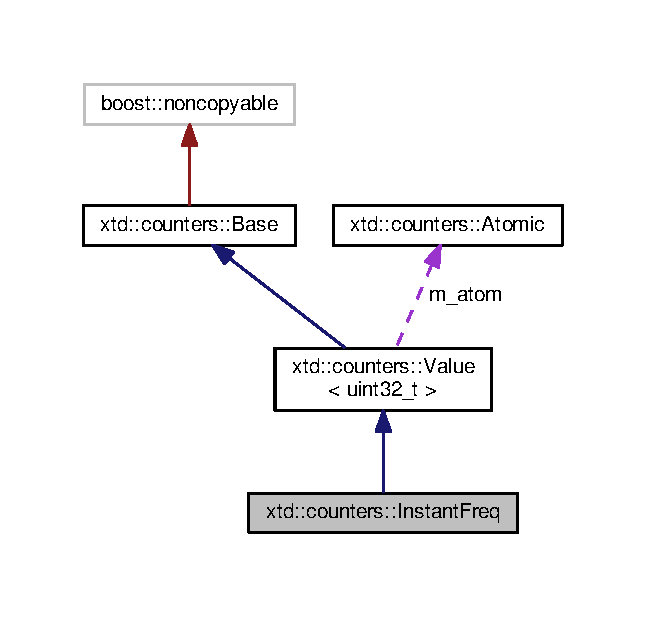
\includegraphics[width=310pt]{classxtd_1_1counters_1_1InstantFreq__coll__graph}
\end{center}
\end{figure}
\subsection*{Public Member Functions}
\begin{DoxyCompactItemize}
\item 
\hyperlink{classxtd_1_1counters_1_1InstantFreq_a428c013f73c1322ee3fc74cc08171c8c}{Instant\-Freq} (const string \&p\-\_\-name, uint32\-\_\-t p\-\_\-time\-Delta\-Ms=1000)
\item 
virtual \hyperlink{classxtd_1_1counters_1_1InstantFreq_a1a002d74711692449aec178e09606193}{$\sim$\-Instant\-Freq} (void)
\item 
void \hyperlink{classxtd_1_1counters_1_1InstantFreq_a1760f09b25b97545169be189bf99d250}{tick} (void)
\item 
\hyperlink{classxtd_1_1counters_1_1InstantFreq}{Instant\-Freq} \& \hyperlink{classxtd_1_1counters_1_1InstantFreq_a3ae7dc13ff6209a0628cdf481ab0a37c}{operator=} (uint32\-\_\-t p\-\_\-value)
\end{DoxyCompactItemize}
\subsection*{Protected Member Functions}
\begin{DoxyCompactItemize}
\item 
void \hyperlink{classxtd_1_1counters_1_1InstantFreq_a2e4629f5a835d7b52425a72f25dcd4d2}{update\-\_\-safe} (void)
\end{DoxyCompactItemize}
\subsection*{Friends}
\begin{DoxyCompactItemize}
\item 
class \hyperlink{classxtd_1_1counters_1_1InstantFreq_a93e934ad70d5b32b14beed5572450abf}{Composed}
\end{DoxyCompactItemize}
\subsection*{Additional Inherited Members}


\subsection{Detailed Description}


Definition at line 13 of file Instant\-Freq.\-hh.



\subsection{Constructor \& Destructor Documentation}
\hypertarget{classxtd_1_1counters_1_1InstantFreq_a428c013f73c1322ee3fc74cc08171c8c}{\index{xtd\-::counters\-::\-Instant\-Freq@{xtd\-::counters\-::\-Instant\-Freq}!Instant\-Freq@{Instant\-Freq}}
\index{Instant\-Freq@{Instant\-Freq}!xtd::counters::InstantFreq@{xtd\-::counters\-::\-Instant\-Freq}}
\subsubsection[{Instant\-Freq}]{\setlength{\rightskip}{0pt plus 5cm}xtd\-::counters\-::\-Instant\-Freq\-::\-Instant\-Freq (
\begin{DoxyParamCaption}
\item[{const string \&}]{p\-\_\-name, }
\item[{uint32\-\_\-t}]{p\-\_\-time\-Delta\-Ms = {\ttfamily 1000}}
\end{DoxyParamCaption}
)}}\label{classxtd_1_1counters_1_1InstantFreq_a428c013f73c1322ee3fc74cc08171c8c}


Definition at line 15 of file Instant\-Freq.\-cc.


\begin{DoxyCode}
16                                                   :
17   \hyperlink{classxtd_1_1counters_1_1Value_a298f146ab57eaed8e6f783c26e78e0f4}{Value}(p\_name),
18   m\_samples(),
19   m\_timeDeltaMs(p\_timeDeltaMs)
20 \{
21 \}
\end{DoxyCode}
\hypertarget{classxtd_1_1counters_1_1InstantFreq_a1a002d74711692449aec178e09606193}{\index{xtd\-::counters\-::\-Instant\-Freq@{xtd\-::counters\-::\-Instant\-Freq}!$\sim$\-Instant\-Freq@{$\sim$\-Instant\-Freq}}
\index{$\sim$\-Instant\-Freq@{$\sim$\-Instant\-Freq}!xtd::counters::InstantFreq@{xtd\-::counters\-::\-Instant\-Freq}}
\subsubsection[{$\sim$\-Instant\-Freq}]{\setlength{\rightskip}{0pt plus 5cm}virtual xtd\-::counters\-::\-Instant\-Freq\-::$\sim$\-Instant\-Freq (
\begin{DoxyParamCaption}
\item[{void}]{}
\end{DoxyParamCaption}
)\hspace{0.3cm}{\ttfamily [inline]}, {\ttfamily [virtual]}}}\label{classxtd_1_1counters_1_1InstantFreq_a1a002d74711692449aec178e09606193}


Definition at line 23 of file Instant\-Freq.\-hh.


\begin{DoxyCode}
23 \{\}
\end{DoxyCode}


\subsection{Member Function Documentation}
\hypertarget{classxtd_1_1counters_1_1InstantFreq_a3ae7dc13ff6209a0628cdf481ab0a37c}{\index{xtd\-::counters\-::\-Instant\-Freq@{xtd\-::counters\-::\-Instant\-Freq}!operator=@{operator=}}
\index{operator=@{operator=}!xtd::counters::InstantFreq@{xtd\-::counters\-::\-Instant\-Freq}}
\subsubsection[{operator=}]{\setlength{\rightskip}{0pt plus 5cm}{\bf Instant\-Freq} \& xtd\-::counters\-::\-Instant\-Freq\-::operator= (
\begin{DoxyParamCaption}
\item[{uint32\-\_\-t}]{p\-\_\-value}
\end{DoxyParamCaption}
)}}\label{classxtd_1_1counters_1_1InstantFreq_a3ae7dc13ff6209a0628cdf481ab0a37c}


Definition at line 34 of file Instant\-Freq.\-cc.


\begin{DoxyCode}
35 \{
36   \hyperlink{classxtd_1_1counters_1_1Value_a017667569f4177e0c44836ef4e9bc7b0}{Value<uint32\_t>::operator=}(p\_value);
37   \textcolor{keywordflow}{return} *\textcolor{keyword}{this};
38 \}
\end{DoxyCode}


Here is the call graph for this function\-:
\nopagebreak
\begin{figure}[H]
\begin{center}
\leavevmode
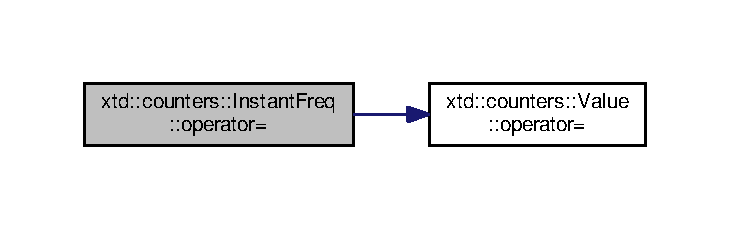
\includegraphics[width=350pt]{classxtd_1_1counters_1_1InstantFreq_a3ae7dc13ff6209a0628cdf481ab0a37c_cgraph}
\end{center}
\end{figure}


\hypertarget{classxtd_1_1counters_1_1InstantFreq_a1760f09b25b97545169be189bf99d250}{\index{xtd\-::counters\-::\-Instant\-Freq@{xtd\-::counters\-::\-Instant\-Freq}!tick@{tick}}
\index{tick@{tick}!xtd::counters::InstantFreq@{xtd\-::counters\-::\-Instant\-Freq}}
\subsubsection[{tick}]{\setlength{\rightskip}{0pt plus 5cm}void xtd\-::counters\-::\-Instant\-Freq\-::tick (
\begin{DoxyParamCaption}
\item[{void}]{}
\end{DoxyParamCaption}
)}}\label{classxtd_1_1counters_1_1InstantFreq_a1760f09b25b97545169be189bf99d250}


Definition at line 24 of file Instant\-Freq.\-cc.


\begin{DoxyCode}
25 \{
26   boost::mutex::scoped\_lock l\_lock(\hyperlink{classxtd_1_1counters_1_1Base_aeeac2ffcae02eb6341418d708188a353}{m\_mutex});
27   bpt::ptime                l\_now = bpt::microsec\_clock::local\_time();
28 
29   m\_samples.push\_front(l\_now);
30   shrink\_safe(l\_now);
31 \}
\end{DoxyCode}


Here is the caller graph for this function\-:
\nopagebreak
\begin{figure}[H]
\begin{center}
\leavevmode
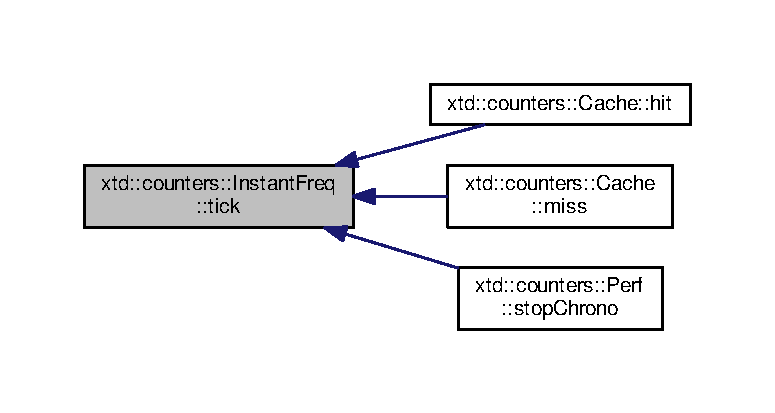
\includegraphics[width=350pt]{classxtd_1_1counters_1_1InstantFreq_a1760f09b25b97545169be189bf99d250_icgraph}
\end{center}
\end{figure}


\hypertarget{classxtd_1_1counters_1_1InstantFreq_a2e4629f5a835d7b52425a72f25dcd4d2}{\index{xtd\-::counters\-::\-Instant\-Freq@{xtd\-::counters\-::\-Instant\-Freq}!update\-\_\-safe@{update\-\_\-safe}}
\index{update\-\_\-safe@{update\-\_\-safe}!xtd::counters::InstantFreq@{xtd\-::counters\-::\-Instant\-Freq}}
\subsubsection[{update\-\_\-safe}]{\setlength{\rightskip}{0pt plus 5cm}void xtd\-::counters\-::\-Instant\-Freq\-::update\-\_\-safe (
\begin{DoxyParamCaption}
\item[{void}]{}
\end{DoxyParamCaption}
)\hspace{0.3cm}{\ttfamily [protected]}, {\ttfamily [virtual]}}}\label{classxtd_1_1counters_1_1InstantFreq_a2e4629f5a835d7b52425a72f25dcd4d2}


Reimplemented from \hyperlink{classxtd_1_1counters_1_1Base_a8b3d10c9fb2bea1d240f887bbe4008ea}{xtd\-::counters\-::\-Base}.



Definition at line 58 of file Instant\-Freq.\-cc.


\begin{DoxyCode}
59 \{
60   bpt::ptime l\_now = bpt::microsec\_clock::local\_time();
61 
62   shrink\_safe(l\_now);
63   \hyperlink{classxtd_1_1counters_1_1Value_abe06c1cebededaf2f216707171f63c3c}{m\_value} = (m\_samples.size() * 1000) / m\_timeDeltaMs;
64 \}
\end{DoxyCode}


\subsection{Friends And Related Function Documentation}
\hypertarget{classxtd_1_1counters_1_1InstantFreq_a93e934ad70d5b32b14beed5572450abf}{\index{xtd\-::counters\-::\-Instant\-Freq@{xtd\-::counters\-::\-Instant\-Freq}!Composed@{Composed}}
\index{Composed@{Composed}!xtd::counters::InstantFreq@{xtd\-::counters\-::\-Instant\-Freq}}
\subsubsection[{Composed}]{\setlength{\rightskip}{0pt plus 5cm}friend class {\bf Composed}\hspace{0.3cm}{\ttfamily [friend]}}}\label{classxtd_1_1counters_1_1InstantFreq_a93e934ad70d5b32b14beed5572450abf}


Definition at line 15 of file Instant\-Freq.\-hh.



The documentation for this class was generated from the following files\-:\begin{DoxyCompactItemize}
\item 
/home/travis/build/psycofdj/xtdcpp/counters/src/\hyperlink{InstantFreq_8hh}{Instant\-Freq.\-hh}\item 
/home/travis/build/psycofdj/xtdcpp/counters/src/\hyperlink{InstantFreq_8cc}{Instant\-Freq.\-cc}\end{DoxyCompactItemize}

\hypertarget{classxtd_1_1counters_1_1JsonVisitor}{}\section{xtd\+:\+:counters\+:\+:Json\+Visitor Class Reference}
\label{classxtd_1_1counters_1_1JsonVisitor}\index{xtd\+::counters\+::\+Json\+Visitor@{xtd\+::counters\+::\+Json\+Visitor}}


{\ttfamily \#include $<$Json\+Visitor.\+hh$>$}



Inheritance diagram for xtd\+:\+:counters\+:\+:Json\+Visitor\+:
\nopagebreak
\begin{figure}[H]
\begin{center}
\leavevmode
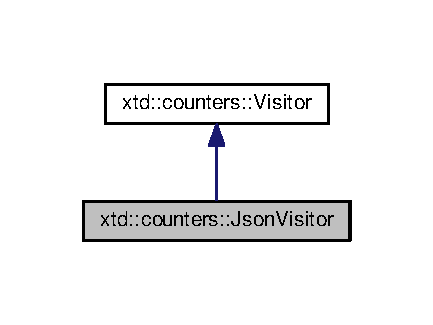
\includegraphics[width=208pt]{classxtd_1_1counters_1_1JsonVisitor__inherit__graph}
\end{center}
\end{figure}


Collaboration diagram for xtd\+:\+:counters\+:\+:Json\+Visitor\+:
\nopagebreak
\begin{figure}[H]
\begin{center}
\leavevmode
\includegraphics[width=208pt]{classxtd_1_1counters_1_1JsonVisitor__coll__graph}
\end{center}
\end{figure}
\subsection*{Public Member Functions}
\begin{DoxyCompactItemize}
\item 
\hyperlink{classxtd_1_1counters_1_1JsonVisitor_a2b3777d2d80ba2c7131afad6385f2433}{Json\+Visitor} (const t\+\_\+path \&p\+\_\+path, t\+\_\+elem \&p\+\_\+elem)
\item 
void \hyperlink{classxtd_1_1counters_1_1JsonVisitor_a903824cfba9c121a0441a774edc232a1}{operator()} (const string \&p\+\_\+name, const string \&p\+\_\+data)
\item 
void \hyperlink{classxtd_1_1counters_1_1JsonVisitor_a6d650a21f6ee33b1748ae7cb432c3de6}{operator()} (const string \&p\+\_\+name, uint8\+\_\+t p\+\_\+data)
\item 
void \hyperlink{classxtd_1_1counters_1_1JsonVisitor_ad0e11fe1f362f071132d6828de269517}{operator()} (const string \&p\+\_\+name, uint16\+\_\+t p\+\_\+data)
\item 
void \hyperlink{classxtd_1_1counters_1_1JsonVisitor_ae9dc018222ce25751d712783377b63a3}{operator()} (const string \&p\+\_\+name, uint32\+\_\+t p\+\_\+data)
\item 
void \hyperlink{classxtd_1_1counters_1_1JsonVisitor_a89f860915a12f1e99b629b5d385864cc}{operator()} (const string \&p\+\_\+name, uint64\+\_\+t p\+\_\+data)
\end{DoxyCompactItemize}


\subsection{Detailed Description}


Definition at line 13 of file Json\+Visitor.\+hh.



\subsection{Constructor \& Destructor Documentation}
\index{xtd\+::counters\+::\+Json\+Visitor@{xtd\+::counters\+::\+Json\+Visitor}!Json\+Visitor@{Json\+Visitor}}
\index{Json\+Visitor@{Json\+Visitor}!xtd\+::counters\+::\+Json\+Visitor@{xtd\+::counters\+::\+Json\+Visitor}}
\subsubsection[{\texorpdfstring{Json\+Visitor(const t\+\_\+path \&p\+\_\+path, t\+\_\+elem \&p\+\_\+elem)}{JsonVisitor(const t_path &p_path, t_elem &p_elem)}}]{\setlength{\rightskip}{0pt plus 5cm}xtd\+::counters\+::\+Json\+Visitor\+::\+Json\+Visitor (
\begin{DoxyParamCaption}
\item[{const t\+\_\+path \&}]{p\+\_\+path, }
\item[{t\+\_\+elem \&}]{p\+\_\+elem}
\end{DoxyParamCaption}
)\hspace{0.3cm}{\ttfamily [inline]}}\hypertarget{classxtd_1_1counters_1_1JsonVisitor_a2b3777d2d80ba2c7131afad6385f2433}{}\label{classxtd_1_1counters_1_1JsonVisitor_a2b3777d2d80ba2c7131afad6385f2433}


Definition at line 20 of file Json\+Visitor.\+hh.


\begin{DoxyCode}
20                                                     :
21     m\_path(p\_path),
22     m\_elem(p\_elem)
23   \{
24   \}
\end{DoxyCode}


\subsection{Member Function Documentation}
\index{xtd\+::counters\+::\+Json\+Visitor@{xtd\+::counters\+::\+Json\+Visitor}!operator()@{operator()}}
\index{operator()@{operator()}!xtd\+::counters\+::\+Json\+Visitor@{xtd\+::counters\+::\+Json\+Visitor}}
\subsubsection[{\texorpdfstring{operator()(const string \&p\+\_\+name, const string \&p\+\_\+data)}{operator()(const string &p_name, const string &p_data)}}]{\setlength{\rightskip}{0pt plus 5cm}void xtd\+::counters\+::\+Json\+Visitor\+::operator() (
\begin{DoxyParamCaption}
\item[{const string \&}]{p\+\_\+name, }
\item[{const string \&}]{p\+\_\+data}
\end{DoxyParamCaption}
)\hspace{0.3cm}{\ttfamily [inline]}, {\ttfamily [virtual]}}\hypertarget{classxtd_1_1counters_1_1JsonVisitor_a903824cfba9c121a0441a774edc232a1}{}\label{classxtd_1_1counters_1_1JsonVisitor_a903824cfba9c121a0441a774edc232a1}


Implements \hyperlink{classxtd_1_1counters_1_1Visitor_a1341281b8c4cbf4de5a37e035f75e214}{xtd\+::counters\+::\+Visitor}.



Definition at line 27 of file Json\+Visitor.\+hh.


\begin{DoxyCode}
27 \{ write(p\_name, p\_data); \}
\end{DoxyCode}
\index{xtd\+::counters\+::\+Json\+Visitor@{xtd\+::counters\+::\+Json\+Visitor}!operator()@{operator()}}
\index{operator()@{operator()}!xtd\+::counters\+::\+Json\+Visitor@{xtd\+::counters\+::\+Json\+Visitor}}
\subsubsection[{\texorpdfstring{operator()(const string \&p\+\_\+name, uint8\+\_\+t p\+\_\+data)}{operator()(const string &p_name, uint8_t p_data)}}]{\setlength{\rightskip}{0pt plus 5cm}void xtd\+::counters\+::\+Json\+Visitor\+::operator() (
\begin{DoxyParamCaption}
\item[{const string \&}]{p\+\_\+name, }
\item[{uint8\+\_\+t}]{p\+\_\+data}
\end{DoxyParamCaption}
)\hspace{0.3cm}{\ttfamily [inline]}, {\ttfamily [virtual]}}\hypertarget{classxtd_1_1counters_1_1JsonVisitor_a6d650a21f6ee33b1748ae7cb432c3de6}{}\label{classxtd_1_1counters_1_1JsonVisitor_a6d650a21f6ee33b1748ae7cb432c3de6}


Implements \hyperlink{classxtd_1_1counters_1_1Visitor_a1a5da2c523703b0c9132595f22e1700e}{xtd\+::counters\+::\+Visitor}.



Definition at line 28 of file Json\+Visitor.\+hh.


\begin{DoxyCode}
28 \{ write(p\_name, p\_data); \}
\end{DoxyCode}
\index{xtd\+::counters\+::\+Json\+Visitor@{xtd\+::counters\+::\+Json\+Visitor}!operator()@{operator()}}
\index{operator()@{operator()}!xtd\+::counters\+::\+Json\+Visitor@{xtd\+::counters\+::\+Json\+Visitor}}
\subsubsection[{\texorpdfstring{operator()(const string \&p\+\_\+name, uint16\+\_\+t p\+\_\+data)}{operator()(const string &p_name, uint16_t p_data)}}]{\setlength{\rightskip}{0pt plus 5cm}void xtd\+::counters\+::\+Json\+Visitor\+::operator() (
\begin{DoxyParamCaption}
\item[{const string \&}]{p\+\_\+name, }
\item[{uint16\+\_\+t}]{p\+\_\+data}
\end{DoxyParamCaption}
)\hspace{0.3cm}{\ttfamily [inline]}, {\ttfamily [virtual]}}\hypertarget{classxtd_1_1counters_1_1JsonVisitor_ad0e11fe1f362f071132d6828de269517}{}\label{classxtd_1_1counters_1_1JsonVisitor_ad0e11fe1f362f071132d6828de269517}


Implements \hyperlink{classxtd_1_1counters_1_1Visitor_a6139d735b720a83e87f49932855f1ade}{xtd\+::counters\+::\+Visitor}.



Definition at line 29 of file Json\+Visitor.\+hh.


\begin{DoxyCode}
29 \{ write(p\_name, p\_data); \}
\end{DoxyCode}
\index{xtd\+::counters\+::\+Json\+Visitor@{xtd\+::counters\+::\+Json\+Visitor}!operator()@{operator()}}
\index{operator()@{operator()}!xtd\+::counters\+::\+Json\+Visitor@{xtd\+::counters\+::\+Json\+Visitor}}
\subsubsection[{\texorpdfstring{operator()(const string \&p\+\_\+name, uint32\+\_\+t p\+\_\+data)}{operator()(const string &p_name, uint32_t p_data)}}]{\setlength{\rightskip}{0pt plus 5cm}void xtd\+::counters\+::\+Json\+Visitor\+::operator() (
\begin{DoxyParamCaption}
\item[{const string \&}]{p\+\_\+name, }
\item[{uint32\+\_\+t}]{p\+\_\+data}
\end{DoxyParamCaption}
)\hspace{0.3cm}{\ttfamily [inline]}, {\ttfamily [virtual]}}\hypertarget{classxtd_1_1counters_1_1JsonVisitor_ae9dc018222ce25751d712783377b63a3}{}\label{classxtd_1_1counters_1_1JsonVisitor_ae9dc018222ce25751d712783377b63a3}


Implements \hyperlink{classxtd_1_1counters_1_1Visitor_a0bc4c30e3df6ef796878b85ce1be17fb}{xtd\+::counters\+::\+Visitor}.



Definition at line 30 of file Json\+Visitor.\+hh.


\begin{DoxyCode}
30 \{ write(p\_name, p\_data); \}
\end{DoxyCode}
\index{xtd\+::counters\+::\+Json\+Visitor@{xtd\+::counters\+::\+Json\+Visitor}!operator()@{operator()}}
\index{operator()@{operator()}!xtd\+::counters\+::\+Json\+Visitor@{xtd\+::counters\+::\+Json\+Visitor}}
\subsubsection[{\texorpdfstring{operator()(const string \&p\+\_\+name, uint64\+\_\+t p\+\_\+data)}{operator()(const string &p_name, uint64_t p_data)}}]{\setlength{\rightskip}{0pt plus 5cm}void xtd\+::counters\+::\+Json\+Visitor\+::operator() (
\begin{DoxyParamCaption}
\item[{const string \&}]{p\+\_\+name, }
\item[{uint64\+\_\+t}]{p\+\_\+data}
\end{DoxyParamCaption}
)\hspace{0.3cm}{\ttfamily [inline]}, {\ttfamily [virtual]}}\hypertarget{classxtd_1_1counters_1_1JsonVisitor_a89f860915a12f1e99b629b5d385864cc}{}\label{classxtd_1_1counters_1_1JsonVisitor_a89f860915a12f1e99b629b5d385864cc}


Implements \hyperlink{classxtd_1_1counters_1_1Visitor_aba895c10dd1a28fa7a8b64e61adee5ac}{xtd\+::counters\+::\+Visitor}.



Definition at line 31 of file Json\+Visitor.\+hh.


\begin{DoxyCode}
31 \{ write(p\_name, p\_data); \}
\end{DoxyCode}


The documentation for this class was generated from the following file\+:\begin{DoxyCompactItemize}
\item 
/home/psyco/dev/xtdcpp/counters/src/\hyperlink{JsonVisitor_8hh}{Json\+Visitor.\+hh}\end{DoxyCompactItemize}

\hypertarget{classxtd_1_1counters_1_1Perf}{}\section{xtd\+:\+:counters\+:\+:Perf Class Reference}
\label{classxtd_1_1counters_1_1Perf}\index{xtd\+::counters\+::\+Perf@{xtd\+::counters\+::\+Perf}}


{\ttfamily \#include $<$Perf.\+hh$>$}



Inheritance diagram for xtd\+:\+:counters\+:\+:Perf\+:
\nopagebreak
\begin{figure}[H]
\begin{center}
\leavevmode
\includegraphics[width=207pt]{classxtd_1_1counters_1_1Perf__inherit__graph}
\end{center}
\end{figure}


Collaboration diagram for xtd\+:\+:counters\+:\+:Perf\+:
\nopagebreak
\begin{figure}[H]
\begin{center}
\leavevmode
\includegraphics[width=207pt]{classxtd_1_1counters_1_1Perf__coll__graph}
\end{center}
\end{figure}
\subsection*{Public Member Functions}
\begin{DoxyCompactItemize}
\item 
\hyperlink{classxtd_1_1counters_1_1Perf_a765416ba7ef076acdfc8100d2ea5c9a0}{Perf} (const string \&p\+\_\+name, uint32\+\_\+t p\+\_\+nb\+Thread, uint32\+\_\+t p\+\_\+sampe\+Size=\hyperlink{classxtd_1_1counters_1_1AvgValue}{Avg\+Value}$<$ uint32\+\_\+t $>$\+::mcs\+\_\+default\+Sample\+Size, uint32\+\_\+t p\+\_\+delta\+Time\+Ms=1000)
\item 
void \hyperlink{classxtd_1_1counters_1_1Perf_a80692e9b90e8d15a57e2e581591063c0}{start\+Chrono} (uint32\+\_\+t p\+\_\+request\+ID)
\item 
void \hyperlink{classxtd_1_1counters_1_1Perf_a905d73c1604d74e28bb56ea2bb4867ef}{stop\+Chrono} (uint32\+\_\+t p\+\_\+request\+ID)
\end{DoxyCompactItemize}
\subsection*{Friends}
\begin{DoxyCompactItemize}
\item 
class \hyperlink{classxtd_1_1counters_1_1Perf_a93e934ad70d5b32b14beed5572450abf}{Composed}
\end{DoxyCompactItemize}
\subsection*{Additional Inherited Members}


\subsection{Detailed Description}
On choisi l\textquotesingle{}heritage plutot que la composition pour garder une coherence sur la visibilite des methodes internes collect\+\_\+safe update\+\_\+safe (qu\textquotesingle{}on serait onbligé de mettre en public ou en friend pour faire de la composition). 

Definition at line 23 of file Perf.\+hh.



\subsection{Constructor \& Destructor Documentation}
\index{xtd\+::counters\+::\+Perf@{xtd\+::counters\+::\+Perf}!Perf@{Perf}}
\index{Perf@{Perf}!xtd\+::counters\+::\+Perf@{xtd\+::counters\+::\+Perf}}
\subsubsection[{\texorpdfstring{Perf(const string \&p\+\_\+name, uint32\+\_\+t p\+\_\+nb\+Thread, uint32\+\_\+t p\+\_\+sampe\+Size=\+Avg\+Value$<$ uint32\+\_\+t $>$\+::mcs\+\_\+default\+Sample\+Size, uint32\+\_\+t p\+\_\+delta\+Time\+Ms=1000)}{Perf(const string &p_name, uint32_t p_nbThread, uint32_t p_sampeSize=AvgValue< uint32_t >::mcs_defaultSampleSize, uint32_t p_deltaTimeMs=1000)}}]{\setlength{\rightskip}{0pt plus 5cm}xtd\+::counters\+::\+Perf\+::\+Perf (
\begin{DoxyParamCaption}
\item[{const string \&}]{p\+\_\+name, }
\item[{uint32\+\_\+t}]{p\+\_\+nb\+Thread, }
\item[{uint32\+\_\+t}]{p\+\_\+sampe\+Size = {\ttfamily {\bf Avg\+Value}$<$uint32\+\_\+t$>$\+:\+:mcs\+\_\+defaultSampleSize}, }
\item[{uint32\+\_\+t}]{p\+\_\+delta\+Time\+Ms = {\ttfamily 1000}}
\end{DoxyParamCaption}
)}\hypertarget{classxtd_1_1counters_1_1Perf_a765416ba7ef076acdfc8100d2ea5c9a0}{}\label{classxtd_1_1counters_1_1Perf_a765416ba7ef076acdfc8100d2ea5c9a0}


Definition at line 13 of file Perf.\+cc.


\begin{DoxyCode}
16                                         :
17   \hyperlink{classxtd_1_1counters_1_1Perf_a93e934ad70d5b32b14beed5572450abf}{Composed}(p\_name),
18   m\_avgRTT(\textcolor{stringliteral}{"RTT"}, p\_sampeSize),
19   m\_globalPerf(\textcolor{stringliteral}{"perf"}),
20   m\_instantPerf(\textcolor{stringliteral}{"instant.perf"}, p\_deltaTimeMs),
21   m\_startTimes(p\_nbThread)
22 \{
23   \hyperlink{classxtd_1_1counters_1_1Composed_ac2efbce59510b352a2d47b3118e0d02a}{addItem}(m\_avgRTT);
24   \hyperlink{classxtd_1_1counters_1_1Composed_ac2efbce59510b352a2d47b3118e0d02a}{addItem}(m\_globalPerf);
25   \hyperlink{classxtd_1_1counters_1_1Composed_ac2efbce59510b352a2d47b3118e0d02a}{addItem}(m\_instantPerf);
26 \}
\end{DoxyCode}


Here is the call graph for this function\+:
\nopagebreak
\begin{figure}[H]
\begin{center}
\leavevmode
\includegraphics[width=341pt]{classxtd_1_1counters_1_1Perf_a765416ba7ef076acdfc8100d2ea5c9a0_cgraph}
\end{center}
\end{figure}




\subsection{Member Function Documentation}
\index{xtd\+::counters\+::\+Perf@{xtd\+::counters\+::\+Perf}!start\+Chrono@{start\+Chrono}}
\index{start\+Chrono@{start\+Chrono}!xtd\+::counters\+::\+Perf@{xtd\+::counters\+::\+Perf}}
\subsubsection[{\texorpdfstring{start\+Chrono(uint32\+\_\+t p\+\_\+request\+I\+D)}{startChrono(uint32_t p_requestID)}}]{\setlength{\rightskip}{0pt plus 5cm}void xtd\+::counters\+::\+Perf\+::start\+Chrono (
\begin{DoxyParamCaption}
\item[{uint32\+\_\+t}]{p\+\_\+request\+ID}
\end{DoxyParamCaption}
)}\hypertarget{classxtd_1_1counters_1_1Perf_a80692e9b90e8d15a57e2e581591063c0}{}\label{classxtd_1_1counters_1_1Perf_a80692e9b90e8d15a57e2e581591063c0}


Definition at line 30 of file Perf.\+cc.


\begin{DoxyCode}
31 \{
32   m\_startTimes[p\_requestID] = bpt::microsec\_clock::local\_time();
33 \}
\end{DoxyCode}
\index{xtd\+::counters\+::\+Perf@{xtd\+::counters\+::\+Perf}!stop\+Chrono@{stop\+Chrono}}
\index{stop\+Chrono@{stop\+Chrono}!xtd\+::counters\+::\+Perf@{xtd\+::counters\+::\+Perf}}
\subsubsection[{\texorpdfstring{stop\+Chrono(uint32\+\_\+t p\+\_\+request\+I\+D)}{stopChrono(uint32_t p_requestID)}}]{\setlength{\rightskip}{0pt plus 5cm}void xtd\+::counters\+::\+Perf\+::stop\+Chrono (
\begin{DoxyParamCaption}
\item[{uint32\+\_\+t}]{p\+\_\+request\+ID}
\end{DoxyParamCaption}
)}\hypertarget{classxtd_1_1counters_1_1Perf_a905d73c1604d74e28bb56ea2bb4867ef}{}\label{classxtd_1_1counters_1_1Perf_a905d73c1604d74e28bb56ea2bb4867ef}


Definition at line 37 of file Perf.\+cc.


\begin{DoxyCode}
38 \{
39   bpt::time\_duration l\_diffTime =
40     bpt::microsec\_clock::local\_time() - m\_startTimes[p\_requestID];
41 
42   m\_globalPerf.\hyperlink{classxtd_1_1counters_1_1Freq_a9e91ea45fc5e9874dc81ca4bd723efc6}{tick}();
43   m\_instantPerf.\hyperlink{classxtd_1_1counters_1_1InstantFreq_a1760f09b25b97545169be189bf99d250}{tick}();
44   m\_avgRTT = l\_diffTime.total\_milliseconds();
45 \}
\end{DoxyCode}


Here is the call graph for this function\+:
\nopagebreak
\begin{figure}[H]
\begin{center}
\leavevmode
\includegraphics[width=343pt]{classxtd_1_1counters_1_1Perf_a905d73c1604d74e28bb56ea2bb4867ef_cgraph}
\end{center}
\end{figure}




\subsection{Friends And Related Function Documentation}
\index{xtd\+::counters\+::\+Perf@{xtd\+::counters\+::\+Perf}!Composed@{Composed}}
\index{Composed@{Composed}!xtd\+::counters\+::\+Perf@{xtd\+::counters\+::\+Perf}}
\subsubsection[{\texorpdfstring{Composed}{Composed}}]{\setlength{\rightskip}{0pt plus 5cm}friend class {\bf Composed}\hspace{0.3cm}{\ttfamily [friend]}}\hypertarget{classxtd_1_1counters_1_1Perf_a93e934ad70d5b32b14beed5572450abf}{}\label{classxtd_1_1counters_1_1Perf_a93e934ad70d5b32b14beed5572450abf}


Definition at line 25 of file Perf.\+hh.



The documentation for this class was generated from the following files\+:\begin{DoxyCompactItemize}
\item 
/home/psyco/dev/xtdcpp/counters/src/\hyperlink{Perf_8hh}{Perf.\+hh}\item 
/home/psyco/dev/xtdcpp/counters/src/\hyperlink{Perf_8cc}{Perf.\+cc}\end{DoxyCompactItemize}

\hypertarget{classxtd_1_1counters_1_1SumExt}{\section{xtd\-:\-:counters\-:\-:Sum\-Ext$<$ T\-Type $>$ Class Template Reference}
\label{classxtd_1_1counters_1_1SumExt}\index{xtd\-::counters\-::\-Sum\-Ext$<$ T\-Type $>$@{xtd\-::counters\-::\-Sum\-Ext$<$ T\-Type $>$}}
}


{\ttfamily \#include $<$counters\-\_\-fwd.\-hh$>$}



Inheritance diagram for xtd\-:\-:counters\-:\-:Sum\-Ext$<$ T\-Type $>$\-:
\nopagebreak
\begin{figure}[H]
\begin{center}
\leavevmode
\includegraphics[width=194pt]{classxtd_1_1counters_1_1SumExt__inherit__graph}
\end{center}
\end{figure}


Collaboration diagram for xtd\-:\-:counters\-:\-:Sum\-Ext$<$ T\-Type $>$\-:
\nopagebreak
\begin{figure}[H]
\begin{center}
\leavevmode
\includegraphics[width=350pt]{classxtd_1_1counters_1_1SumExt__coll__graph}
\end{center}
\end{figure}
\subsection*{Public Member Functions}
\begin{DoxyCompactItemize}
\item 
\hyperlink{classxtd_1_1counters_1_1SumExt_aeed4a5cca01073d91a3c24212618ab9e}{Sum\-Ext} (const string \&p\-\_\-name)
\item 
virtual \hyperlink{classxtd_1_1counters_1_1SumExt_a304ba48e158f8f75120b9449300c688a}{$\sim$\-Sum\-Ext} (void)
\item 
void \hyperlink{classxtd_1_1counters_1_1SumExt_a05b01643f8724ccdfd98f8a3209dc99c}{add\-Item} (const T\-Type \&p\-\_\-val)
\end{DoxyCompactItemize}
\subsection*{Protected Member Functions}
\begin{DoxyCompactItemize}
\item 
virtual void \hyperlink{classxtd_1_1counters_1_1SumExt_a1f3c5d348aa4b16104027fb2175acbe6}{update\-\_\-safe} (void)
\end{DoxyCompactItemize}
\subsection*{Friends}
\begin{DoxyCompactItemize}
\item 
class \hyperlink{classxtd_1_1counters_1_1SumExt_a93e934ad70d5b32b14beed5572450abf}{Composed}
\end{DoxyCompactItemize}
\subsection*{Additional Inherited Members}


\subsection{Detailed Description}
\subsubsection*{template$<$typename T\-Type$>$class xtd\-::counters\-::\-Sum\-Ext$<$ T\-Type $>$}



Definition at line 12 of file counters\-\_\-fwd.\-hh.



\subsection{Constructor \& Destructor Documentation}
\hypertarget{classxtd_1_1counters_1_1SumExt_aeed4a5cca01073d91a3c24212618ab9e}{\index{xtd\-::counters\-::\-Sum\-Ext@{xtd\-::counters\-::\-Sum\-Ext}!Sum\-Ext@{Sum\-Ext}}
\index{Sum\-Ext@{Sum\-Ext}!xtd::counters::SumExt@{xtd\-::counters\-::\-Sum\-Ext}}
\subsubsection[{Sum\-Ext}]{\setlength{\rightskip}{0pt plus 5cm}template$<$typename T\-Type $>$ {\bf xtd\-::counters\-::\-Sum\-Ext}$<$ T\-Type $>$\-::{\bf Sum\-Ext} (
\begin{DoxyParamCaption}
\item[{const string \&}]{p\-\_\-name}
\end{DoxyParamCaption}
)}}\label{classxtd_1_1counters_1_1SumExt_aeed4a5cca01073d91a3c24212618ab9e}
\hypertarget{classxtd_1_1counters_1_1SumExt_a304ba48e158f8f75120b9449300c688a}{\index{xtd\-::counters\-::\-Sum\-Ext@{xtd\-::counters\-::\-Sum\-Ext}!$\sim$\-Sum\-Ext@{$\sim$\-Sum\-Ext}}
\index{$\sim$\-Sum\-Ext@{$\sim$\-Sum\-Ext}!xtd::counters::SumExt@{xtd\-::counters\-::\-Sum\-Ext}}
\subsubsection[{$\sim$\-Sum\-Ext}]{\setlength{\rightskip}{0pt plus 5cm}template$<$typename T\-Type $>$ virtual {\bf xtd\-::counters\-::\-Sum\-Ext}$<$ T\-Type $>$\-::$\sim${\bf Sum\-Ext} (
\begin{DoxyParamCaption}
\item[{void}]{}
\end{DoxyParamCaption}
)\hspace{0.3cm}{\ttfamily [inline]}, {\ttfamily [virtual]}}}\label{classxtd_1_1counters_1_1SumExt_a304ba48e158f8f75120b9449300c688a}


Definition at line 22 of file Sum\-Ext.\-hh.


\begin{DoxyCode}
22 \{\};
\end{DoxyCode}


\subsection{Member Function Documentation}
\hypertarget{classxtd_1_1counters_1_1SumExt_a05b01643f8724ccdfd98f8a3209dc99c}{\index{xtd\-::counters\-::\-Sum\-Ext@{xtd\-::counters\-::\-Sum\-Ext}!add\-Item@{add\-Item}}
\index{add\-Item@{add\-Item}!xtd::counters::SumExt@{xtd\-::counters\-::\-Sum\-Ext}}
\subsubsection[{add\-Item}]{\setlength{\rightskip}{0pt plus 5cm}template$<$typename T\-Type $>$ void {\bf xtd\-::counters\-::\-Sum\-Ext}$<$ T\-Type $>$\-::add\-Item (
\begin{DoxyParamCaption}
\item[{const T\-Type \&}]{p\-\_\-val}
\end{DoxyParamCaption}
)}}\label{classxtd_1_1counters_1_1SumExt_a05b01643f8724ccdfd98f8a3209dc99c}
\hypertarget{classxtd_1_1counters_1_1SumExt_a1f3c5d348aa4b16104027fb2175acbe6}{\index{xtd\-::counters\-::\-Sum\-Ext@{xtd\-::counters\-::\-Sum\-Ext}!update\-\_\-safe@{update\-\_\-safe}}
\index{update\-\_\-safe@{update\-\_\-safe}!xtd::counters::SumExt@{xtd\-::counters\-::\-Sum\-Ext}}
\subsubsection[{update\-\_\-safe}]{\setlength{\rightskip}{0pt plus 5cm}template$<$typename T\-Type $>$ virtual void {\bf xtd\-::counters\-::\-Sum\-Ext}$<$ T\-Type $>$\-::update\-\_\-safe (
\begin{DoxyParamCaption}
\item[{void}]{}
\end{DoxyParamCaption}
)\hspace{0.3cm}{\ttfamily [protected]}, {\ttfamily [virtual]}}}\label{classxtd_1_1counters_1_1SumExt_a1f3c5d348aa4b16104027fb2175acbe6}


Reimplemented from \hyperlink{classxtd_1_1counters_1_1Base_a8b3d10c9fb2bea1d240f887bbe4008ea}{xtd\-::counters\-::\-Base}.



\subsection{Friends And Related Function Documentation}
\hypertarget{classxtd_1_1counters_1_1SumExt_a93e934ad70d5b32b14beed5572450abf}{\index{xtd\-::counters\-::\-Sum\-Ext@{xtd\-::counters\-::\-Sum\-Ext}!Composed@{Composed}}
\index{Composed@{Composed}!xtd::counters::SumExt@{xtd\-::counters\-::\-Sum\-Ext}}
\subsubsection[{Composed}]{\setlength{\rightskip}{0pt plus 5cm}template$<$typename T\-Type $>$ friend class {\bf Composed}\hspace{0.3cm}{\ttfamily [friend]}}}\label{classxtd_1_1counters_1_1SumExt_a93e934ad70d5b32b14beed5572450abf}


Definition at line 15 of file Sum\-Ext.\-hh.



The documentation for this class was generated from the following files\-:\begin{DoxyCompactItemize}
\item 
/home/travis/build/psycofdj/xtdcpp/counters/src/\hyperlink{counters__fwd_8hh}{counters\-\_\-fwd.\-hh}\item 
/home/travis/build/psycofdj/xtdcpp/counters/src/\hyperlink{SumExt_8hh}{Sum\-Ext.\-hh}\end{DoxyCompactItemize}

\hypertarget{classxtd_1_1counters_1_1Value}{\section{xtd\-:\-:counters\-:\-:Value$<$ T\-Type $>$ Class Template Reference}
\label{classxtd_1_1counters_1_1Value}\index{xtd\-::counters\-::\-Value$<$ T\-Type $>$@{xtd\-::counters\-::\-Value$<$ T\-Type $>$}}
}


{\ttfamily \#include $<$counters\-\_\-fwd.\-hh$>$}



Inheritance diagram for xtd\-:\-:counters\-:\-:Value$<$ T\-Type $>$\-:
\nopagebreak
\begin{figure}[H]
\begin{center}
\leavevmode
\includegraphics[width=194pt]{classxtd_1_1counters_1_1Value__inherit__graph}
\end{center}
\end{figure}


Collaboration diagram for xtd\-:\-:counters\-:\-:Value$<$ T\-Type $>$\-:
\nopagebreak
\begin{figure}[H]
\begin{center}
\leavevmode
\includegraphics[width=350pt]{classxtd_1_1counters_1_1Value__coll__graph}
\end{center}
\end{figure}
\subsection*{Public Types}
\begin{DoxyCompactItemize}
\item 
typedef boost\-::shared\-\_\-ptr\\*
$<$ \hyperlink{classxtd_1_1counters_1_1Value}{Value}$<$ T\-Type $>$ $>$ \hyperlink{classxtd_1_1counters_1_1Value_a24669b6d950db6c5c20546ce12a467cf}{t\-\_\-sptr}
\end{DoxyCompactItemize}
\subsection*{Public Member Functions}
\begin{DoxyCompactItemize}
\item 
\hyperlink{classxtd_1_1counters_1_1Value_a298f146ab57eaed8e6f783c26e78e0f4}{Value} (const string \&p\-\_\-name)
\item 
virtual \hyperlink{classxtd_1_1counters_1_1Value_a500d43a2cea3f654aa524959a7893e31}{$\sim$\-Value} (void)
\item 
\hyperlink{classxtd_1_1counters_1_1Value}{Value} \& \hyperlink{classxtd_1_1counters_1_1Value_ab206db077ef38ac776a7e64774f56f2b}{Na\-N} (void)
\item 
bool \hyperlink{classxtd_1_1counters_1_1Value_a6fab70b05b6e99db492e0a3d8a0d9fb6}{is\-Na\-N} (void) const 
\item 
\hyperlink{classxtd_1_1counters_1_1Value}{Value} \& \hyperlink{classxtd_1_1counters_1_1Value_a017667569f4177e0c44836ef4e9bc7b0}{operator=} (const T\-Type \&p\-\_\-value)
\item 
\hyperlink{classxtd_1_1counters_1_1Value}{Value} \& \hyperlink{classxtd_1_1counters_1_1Value_a8e7e5f0ff7388f18deaddf51e016c905}{operator++} (void)
\item 
\hyperlink{classxtd_1_1counters_1_1Value}{Value} \& \hyperlink{classxtd_1_1counters_1_1Value_a4a8989a7f9585998eb4210dfdd1b099e}{operator++} (int)
\item 
\hyperlink{classxtd_1_1counters_1_1Value}{Value} \& \hyperlink{classxtd_1_1counters_1_1Value_ac94ea7115378eb16dbef10d030b52a66}{operator-\/-\/} (void)
\item 
\hyperlink{classxtd_1_1counters_1_1Value}{Value} \& \hyperlink{classxtd_1_1counters_1_1Value_a9036f1b2a2904960e67c1faef11f1835}{operator-\/-\/} (int)
\item 
const T\-Type \& \hyperlink{classxtd_1_1counters_1_1Value_a459b2e9fc6974821968f5c05a62ec4ca}{get\-Value} (void) const 
\end{DoxyCompactItemize}
\subsection*{Protected Member Functions}
\begin{DoxyCompactItemize}
\item 
void \hyperlink{classxtd_1_1counters_1_1Value_a7be35e9a5a52891c5946425152b4db30}{visit\-\_\-safe} (\hyperlink{classxtd_1_1counters_1_1Visitor}{Visitor} \&p\-\_\-visitor) const 
\end{DoxyCompactItemize}
\subsection*{Protected Attributes}
\begin{DoxyCompactItemize}
\item 
bool \hyperlink{classxtd_1_1counters_1_1Value_a28be66961121bb488351e2c2722fd18a}{m\-\_\-is\-Na\-N}
\item 
T\-Type \hyperlink{classxtd_1_1counters_1_1Value_abe06c1cebededaf2f216707171f63c3c}{m\-\_\-value}
\item 
\hyperlink{classxtd_1_1counters_1_1Atomic}{Atomic} \hyperlink{classxtd_1_1counters_1_1Value_a0cf45c8f82588321af127529ba4f214a}{m\-\_\-atom}
\end{DoxyCompactItemize}
\subsection*{Friends}
\begin{DoxyCompactItemize}
\item 
class \hyperlink{classxtd_1_1counters_1_1Value_a93e934ad70d5b32b14beed5572450abf}{Composed}
\end{DoxyCompactItemize}


\subsection{Detailed Description}
\subsubsection*{template$<$typename T\-Type$>$class xtd\-::counters\-::\-Value$<$ T\-Type $>$}



Definition at line 9 of file counters\-\_\-fwd.\-hh.



\subsection{Member Typedef Documentation}
\hypertarget{classxtd_1_1counters_1_1Value_a24669b6d950db6c5c20546ce12a467cf}{\index{xtd\-::counters\-::\-Value@{xtd\-::counters\-::\-Value}!t\-\_\-sptr@{t\-\_\-sptr}}
\index{t\-\_\-sptr@{t\-\_\-sptr}!xtd::counters::Value@{xtd\-::counters\-::\-Value}}
\subsubsection[{t\-\_\-sptr}]{\setlength{\rightskip}{0pt plus 5cm}template$<$typename T\-Type$>$ typedef boost\-::shared\-\_\-ptr$<${\bf Value}$<$T\-Type$>$ $>$ {\bf xtd\-::counters\-::\-Value}$<$ T\-Type $>$\-::{\bf t\-\_\-sptr}}}\label{classxtd_1_1counters_1_1Value_a24669b6d950db6c5c20546ce12a467cf}


Definition at line 41 of file Value.\-hh.



\subsection{Constructor \& Destructor Documentation}
\hypertarget{classxtd_1_1counters_1_1Value_a298f146ab57eaed8e6f783c26e78e0f4}{\index{xtd\-::counters\-::\-Value@{xtd\-::counters\-::\-Value}!Value@{Value}}
\index{Value@{Value}!xtd::counters::Value@{xtd\-::counters\-::\-Value}}
\subsubsection[{Value}]{\setlength{\rightskip}{0pt plus 5cm}template$<$typename T\-Type$>$ {\bf xtd\-::counters\-::\-Value}$<$ T\-Type $>$\-::{\bf Value} (
\begin{DoxyParamCaption}
\item[{const string \&}]{p\-\_\-name}
\end{DoxyParamCaption}
)}}\label{classxtd_1_1counters_1_1Value_a298f146ab57eaed8e6f783c26e78e0f4}
\hypertarget{classxtd_1_1counters_1_1Value_a500d43a2cea3f654aa524959a7893e31}{\index{xtd\-::counters\-::\-Value@{xtd\-::counters\-::\-Value}!$\sim$\-Value@{$\sim$\-Value}}
\index{$\sim$\-Value@{$\sim$\-Value}!xtd::counters::Value@{xtd\-::counters\-::\-Value}}
\subsubsection[{$\sim$\-Value}]{\setlength{\rightskip}{0pt plus 5cm}template$<$typename T\-Type$>$ virtual {\bf xtd\-::counters\-::\-Value}$<$ T\-Type $>$\-::$\sim${\bf Value} (
\begin{DoxyParamCaption}
\item[{void}]{}
\end{DoxyParamCaption}
)\hspace{0.3cm}{\ttfamily [inline]}, {\ttfamily [virtual]}}}\label{classxtd_1_1counters_1_1Value_a500d43a2cea3f654aa524959a7893e31}


Definition at line 45 of file Value.\-hh.


\begin{DoxyCode}
45 \{\};
\end{DoxyCode}


\subsection{Member Function Documentation}
\hypertarget{classxtd_1_1counters_1_1Value_a459b2e9fc6974821968f5c05a62ec4ca}{\index{xtd\-::counters\-::\-Value@{xtd\-::counters\-::\-Value}!get\-Value@{get\-Value}}
\index{get\-Value@{get\-Value}!xtd::counters::Value@{xtd\-::counters\-::\-Value}}
\subsubsection[{get\-Value}]{\setlength{\rightskip}{0pt plus 5cm}template$<$typename T\-Type$>$ const T\-Type\& {\bf xtd\-::counters\-::\-Value}$<$ T\-Type $>$\-::get\-Value (
\begin{DoxyParamCaption}
\item[{void}]{}
\end{DoxyParamCaption}
) const}}\label{classxtd_1_1counters_1_1Value_a459b2e9fc6974821968f5c05a62ec4ca}
\hypertarget{classxtd_1_1counters_1_1Value_a6fab70b05b6e99db492e0a3d8a0d9fb6}{\index{xtd\-::counters\-::\-Value@{xtd\-::counters\-::\-Value}!is\-Na\-N@{is\-Na\-N}}
\index{is\-Na\-N@{is\-Na\-N}!xtd::counters::Value@{xtd\-::counters\-::\-Value}}
\subsubsection[{is\-Na\-N}]{\setlength{\rightskip}{0pt plus 5cm}template$<$typename T\-Type$>$ bool {\bf xtd\-::counters\-::\-Value}$<$ T\-Type $>$\-::is\-Na\-N (
\begin{DoxyParamCaption}
\item[{void}]{}
\end{DoxyParamCaption}
) const}}\label{classxtd_1_1counters_1_1Value_a6fab70b05b6e99db492e0a3d8a0d9fb6}
\hypertarget{classxtd_1_1counters_1_1Value_ab206db077ef38ac776a7e64774f56f2b}{\index{xtd\-::counters\-::\-Value@{xtd\-::counters\-::\-Value}!Na\-N@{Na\-N}}
\index{Na\-N@{Na\-N}!xtd::counters::Value@{xtd\-::counters\-::\-Value}}
\subsubsection[{Na\-N}]{\setlength{\rightskip}{0pt plus 5cm}template$<$typename T\-Type$>$ {\bf Value}\& {\bf xtd\-::counters\-::\-Value}$<$ T\-Type $>$\-::Na\-N (
\begin{DoxyParamCaption}
\item[{void}]{}
\end{DoxyParamCaption}
)}}\label{classxtd_1_1counters_1_1Value_ab206db077ef38ac776a7e64774f56f2b}


Here is the caller graph for this function\-:
\nopagebreak
\begin{figure}[H]
\begin{center}
\leavevmode
\includegraphics[width=350pt]{classxtd_1_1counters_1_1Value_ab206db077ef38ac776a7e64774f56f2b_icgraph}
\end{center}
\end{figure}


\hypertarget{classxtd_1_1counters_1_1Value_a8e7e5f0ff7388f18deaddf51e016c905}{\index{xtd\-::counters\-::\-Value@{xtd\-::counters\-::\-Value}!operator++@{operator++}}
\index{operator++@{operator++}!xtd::counters::Value@{xtd\-::counters\-::\-Value}}
\subsubsection[{operator++}]{\setlength{\rightskip}{0pt plus 5cm}template$<$typename T\-Type$>$ {\bf Value}\& {\bf xtd\-::counters\-::\-Value}$<$ T\-Type $>$\-::operator++ (
\begin{DoxyParamCaption}
\item[{void}]{}
\end{DoxyParamCaption}
)}}\label{classxtd_1_1counters_1_1Value_a8e7e5f0ff7388f18deaddf51e016c905}
\hypertarget{classxtd_1_1counters_1_1Value_a4a8989a7f9585998eb4210dfdd1b099e}{\index{xtd\-::counters\-::\-Value@{xtd\-::counters\-::\-Value}!operator++@{operator++}}
\index{operator++@{operator++}!xtd::counters::Value@{xtd\-::counters\-::\-Value}}
\subsubsection[{operator++}]{\setlength{\rightskip}{0pt plus 5cm}template$<$typename T\-Type$>$ {\bf Value}\& {\bf xtd\-::counters\-::\-Value}$<$ T\-Type $>$\-::operator++ (
\begin{DoxyParamCaption}
\item[{int}]{}
\end{DoxyParamCaption}
)}}\label{classxtd_1_1counters_1_1Value_a4a8989a7f9585998eb4210dfdd1b099e}
\hypertarget{classxtd_1_1counters_1_1Value_ac94ea7115378eb16dbef10d030b52a66}{\index{xtd\-::counters\-::\-Value@{xtd\-::counters\-::\-Value}!operator-\/-\/@{operator-\/-\/}}
\index{operator-\/-\/@{operator-\/-\/}!xtd::counters::Value@{xtd\-::counters\-::\-Value}}
\subsubsection[{operator-\/-\/}]{\setlength{\rightskip}{0pt plus 5cm}template$<$typename T\-Type$>$ {\bf Value}\& {\bf xtd\-::counters\-::\-Value}$<$ T\-Type $>$\-::operator-\/-\/ (
\begin{DoxyParamCaption}
\item[{void}]{}
\end{DoxyParamCaption}
)}}\label{classxtd_1_1counters_1_1Value_ac94ea7115378eb16dbef10d030b52a66}
\hypertarget{classxtd_1_1counters_1_1Value_a9036f1b2a2904960e67c1faef11f1835}{\index{xtd\-::counters\-::\-Value@{xtd\-::counters\-::\-Value}!operator-\/-\/@{operator-\/-\/}}
\index{operator-\/-\/@{operator-\/-\/}!xtd::counters::Value@{xtd\-::counters\-::\-Value}}
\subsubsection[{operator-\/-\/}]{\setlength{\rightskip}{0pt plus 5cm}template$<$typename T\-Type$>$ {\bf Value}\& {\bf xtd\-::counters\-::\-Value}$<$ T\-Type $>$\-::operator-\/-\/ (
\begin{DoxyParamCaption}
\item[{int}]{}
\end{DoxyParamCaption}
)}}\label{classxtd_1_1counters_1_1Value_a9036f1b2a2904960e67c1faef11f1835}
\hypertarget{classxtd_1_1counters_1_1Value_a017667569f4177e0c44836ef4e9bc7b0}{\index{xtd\-::counters\-::\-Value@{xtd\-::counters\-::\-Value}!operator=@{operator=}}
\index{operator=@{operator=}!xtd::counters::Value@{xtd\-::counters\-::\-Value}}
\subsubsection[{operator=}]{\setlength{\rightskip}{0pt plus 5cm}template$<$typename T\-Type$>$ {\bf Value}\& {\bf xtd\-::counters\-::\-Value}$<$ T\-Type $>$\-::operator= (
\begin{DoxyParamCaption}
\item[{const T\-Type \&}]{p\-\_\-value}
\end{DoxyParamCaption}
)}}\label{classxtd_1_1counters_1_1Value_a017667569f4177e0c44836ef4e9bc7b0}


Here is the caller graph for this function\-:
\nopagebreak
\begin{figure}[H]
\begin{center}
\leavevmode
\includegraphics[width=350pt]{classxtd_1_1counters_1_1Value_a017667569f4177e0c44836ef4e9bc7b0_icgraph}
\end{center}
\end{figure}


\hypertarget{classxtd_1_1counters_1_1Value_a7be35e9a5a52891c5946425152b4db30}{\index{xtd\-::counters\-::\-Value@{xtd\-::counters\-::\-Value}!visit\-\_\-safe@{visit\-\_\-safe}}
\index{visit\-\_\-safe@{visit\-\_\-safe}!xtd::counters::Value@{xtd\-::counters\-::\-Value}}
\subsubsection[{visit\-\_\-safe}]{\setlength{\rightskip}{0pt plus 5cm}template$<$typename T\-Type$>$ void {\bf xtd\-::counters\-::\-Value}$<$ T\-Type $>$\-::visit\-\_\-safe (
\begin{DoxyParamCaption}
\item[{{\bf Visitor} \&}]{p\-\_\-visitor}
\end{DoxyParamCaption}
) const\hspace{0.3cm}{\ttfamily [protected]}, {\ttfamily [virtual]}}}\label{classxtd_1_1counters_1_1Value_a7be35e9a5a52891c5946425152b4db30}


Implements \hyperlink{classxtd_1_1counters_1_1Base_a0b8f3bdc6880dc03da750aa815dfdf0b}{xtd\-::counters\-::\-Base}.



\subsection{Friends And Related Function Documentation}
\hypertarget{classxtd_1_1counters_1_1Value_a93e934ad70d5b32b14beed5572450abf}{\index{xtd\-::counters\-::\-Value@{xtd\-::counters\-::\-Value}!Composed@{Composed}}
\index{Composed@{Composed}!xtd::counters::Value@{xtd\-::counters\-::\-Value}}
\subsubsection[{Composed}]{\setlength{\rightskip}{0pt plus 5cm}template$<$typename T\-Type$>$ friend class {\bf Composed}\hspace{0.3cm}{\ttfamily [friend]}}}\label{classxtd_1_1counters_1_1Value_a93e934ad70d5b32b14beed5572450abf}


Definition at line 38 of file Value.\-hh.



\subsection{Member Data Documentation}
\hypertarget{classxtd_1_1counters_1_1Value_a0cf45c8f82588321af127529ba4f214a}{\index{xtd\-::counters\-::\-Value@{xtd\-::counters\-::\-Value}!m\-\_\-atom@{m\-\_\-atom}}
\index{m\-\_\-atom@{m\-\_\-atom}!xtd::counters::Value@{xtd\-::counters\-::\-Value}}
\subsubsection[{m\-\_\-atom}]{\setlength{\rightskip}{0pt plus 5cm}template$<$typename T\-Type$>$ {\bf Atomic} {\bf xtd\-::counters\-::\-Value}$<$ T\-Type $>$\-::m\-\_\-atom\hspace{0.3cm}{\ttfamily [protected]}}}\label{classxtd_1_1counters_1_1Value_a0cf45c8f82588321af127529ba4f214a}


Definition at line 65 of file Value.\-hh.

\hypertarget{classxtd_1_1counters_1_1Value_a28be66961121bb488351e2c2722fd18a}{\index{xtd\-::counters\-::\-Value@{xtd\-::counters\-::\-Value}!m\-\_\-is\-Na\-N@{m\-\_\-is\-Na\-N}}
\index{m\-\_\-is\-Na\-N@{m\-\_\-is\-Na\-N}!xtd::counters::Value@{xtd\-::counters\-::\-Value}}
\subsubsection[{m\-\_\-is\-Na\-N}]{\setlength{\rightskip}{0pt plus 5cm}template$<$typename T\-Type$>$ bool {\bf xtd\-::counters\-::\-Value}$<$ T\-Type $>$\-::m\-\_\-is\-Na\-N\hspace{0.3cm}{\ttfamily [protected]}}}\label{classxtd_1_1counters_1_1Value_a28be66961121bb488351e2c2722fd18a}


Definition at line 63 of file Value.\-hh.

\hypertarget{classxtd_1_1counters_1_1Value_abe06c1cebededaf2f216707171f63c3c}{\index{xtd\-::counters\-::\-Value@{xtd\-::counters\-::\-Value}!m\-\_\-value@{m\-\_\-value}}
\index{m\-\_\-value@{m\-\_\-value}!xtd::counters::Value@{xtd\-::counters\-::\-Value}}
\subsubsection[{m\-\_\-value}]{\setlength{\rightskip}{0pt plus 5cm}template$<$typename T\-Type$>$ T\-Type {\bf xtd\-::counters\-::\-Value}$<$ T\-Type $>$\-::m\-\_\-value\hspace{0.3cm}{\ttfamily [protected]}}}\label{classxtd_1_1counters_1_1Value_abe06c1cebededaf2f216707171f63c3c}


Definition at line 64 of file Value.\-hh.



The documentation for this class was generated from the following files\-:\begin{DoxyCompactItemize}
\item 
/home/travis/build/psycofdj/xtdcpp/counters/src/\hyperlink{counters__fwd_8hh}{counters\-\_\-fwd.\-hh}\item 
/home/travis/build/psycofdj/xtdcpp/counters/src/\hyperlink{Value_8hh}{Value.\-hh}\end{DoxyCompactItemize}

\hypertarget{classxtd_1_1counters_1_1Visitor}{}\section{xtd\+:\+:counters\+:\+:Visitor Class Reference}
\label{classxtd_1_1counters_1_1Visitor}\index{xtd\+::counters\+::\+Visitor@{xtd\+::counters\+::\+Visitor}}


{\ttfamily \#include $<$Visitor.\+hh$>$}



Inheritance diagram for xtd\+:\+:counters\+:\+:Visitor\+:
\nopagebreak
\begin{figure}[H]
\begin{center}
\leavevmode
\includegraphics[width=350pt]{classxtd_1_1counters_1_1Visitor__inherit__graph}
\end{center}
\end{figure}
\subsection*{Public Member Functions}
\begin{DoxyCompactItemize}
\item 
virtual void \hyperlink{classxtd_1_1counters_1_1Visitor_a1341281b8c4cbf4de5a37e035f75e214}{operator()} (const string \&, const string \&)=0
\item 
virtual void \hyperlink{classxtd_1_1counters_1_1Visitor_a1a5da2c523703b0c9132595f22e1700e}{operator()} (const string \&, uint8\+\_\+t)=0
\item 
virtual void \hyperlink{classxtd_1_1counters_1_1Visitor_a6139d735b720a83e87f49932855f1ade}{operator()} (const string \&, uint16\+\_\+t)=0
\item 
virtual void \hyperlink{classxtd_1_1counters_1_1Visitor_a0bc4c30e3df6ef796878b85ce1be17fb}{operator()} (const string \&, uint32\+\_\+t)=0
\item 
virtual void \hyperlink{classxtd_1_1counters_1_1Visitor_aba895c10dd1a28fa7a8b64e61adee5ac}{operator()} (const string \&, uint64\+\_\+t)=0
\end{DoxyCompactItemize}


\subsection{Detailed Description}


Definition at line 9 of file Visitor.\+hh.



\subsection{Member Function Documentation}
\index{xtd\+::counters\+::\+Visitor@{xtd\+::counters\+::\+Visitor}!operator()@{operator()}}
\index{operator()@{operator()}!xtd\+::counters\+::\+Visitor@{xtd\+::counters\+::\+Visitor}}
\subsubsection[{\texorpdfstring{operator()(const string \&, const string \&)=0}{operator()(const string &, const string &)=0}}]{\setlength{\rightskip}{0pt plus 5cm}virtual void xtd\+::counters\+::\+Visitor\+::operator() (
\begin{DoxyParamCaption}
\item[{const string \&}]{, }
\item[{const string \&}]{}
\end{DoxyParamCaption}
)\hspace{0.3cm}{\ttfamily [pure virtual]}}\hypertarget{classxtd_1_1counters_1_1Visitor_a1341281b8c4cbf4de5a37e035f75e214}{}\label{classxtd_1_1counters_1_1Visitor_a1341281b8c4cbf4de5a37e035f75e214}


Implemented in \hyperlink{classxtd_1_1counters_1_1JsonVisitor_a903824cfba9c121a0441a774edc232a1}{xtd\+::counters\+::\+Json\+Visitor}, and \hyperlink{classxtd_1_1counters_1_1FileVisitor_af6936e3e1e62880b0eb9fc76b0b0a120}{xtd\+::counters\+::\+File\+Visitor}.

\index{xtd\+::counters\+::\+Visitor@{xtd\+::counters\+::\+Visitor}!operator()@{operator()}}
\index{operator()@{operator()}!xtd\+::counters\+::\+Visitor@{xtd\+::counters\+::\+Visitor}}
\subsubsection[{\texorpdfstring{operator()(const string \&, uint8\+\_\+t)=0}{operator()(const string &, uint8_t)=0}}]{\setlength{\rightskip}{0pt plus 5cm}virtual void xtd\+::counters\+::\+Visitor\+::operator() (
\begin{DoxyParamCaption}
\item[{const string \&}]{, }
\item[{uint8\+\_\+t}]{}
\end{DoxyParamCaption}
)\hspace{0.3cm}{\ttfamily [pure virtual]}}\hypertarget{classxtd_1_1counters_1_1Visitor_a1a5da2c523703b0c9132595f22e1700e}{}\label{classxtd_1_1counters_1_1Visitor_a1a5da2c523703b0c9132595f22e1700e}


Implemented in \hyperlink{classxtd_1_1counters_1_1JsonVisitor_a6d650a21f6ee33b1748ae7cb432c3de6}{xtd\+::counters\+::\+Json\+Visitor}, and \hyperlink{classxtd_1_1counters_1_1FileVisitor_a69214d261c695bb48335c58ed2a76cae}{xtd\+::counters\+::\+File\+Visitor}.

\index{xtd\+::counters\+::\+Visitor@{xtd\+::counters\+::\+Visitor}!operator()@{operator()}}
\index{operator()@{operator()}!xtd\+::counters\+::\+Visitor@{xtd\+::counters\+::\+Visitor}}
\subsubsection[{\texorpdfstring{operator()(const string \&, uint16\+\_\+t)=0}{operator()(const string &, uint16_t)=0}}]{\setlength{\rightskip}{0pt plus 5cm}virtual void xtd\+::counters\+::\+Visitor\+::operator() (
\begin{DoxyParamCaption}
\item[{const string \&}]{, }
\item[{uint16\+\_\+t}]{}
\end{DoxyParamCaption}
)\hspace{0.3cm}{\ttfamily [pure virtual]}}\hypertarget{classxtd_1_1counters_1_1Visitor_a6139d735b720a83e87f49932855f1ade}{}\label{classxtd_1_1counters_1_1Visitor_a6139d735b720a83e87f49932855f1ade}


Implemented in \hyperlink{classxtd_1_1counters_1_1JsonVisitor_ad0e11fe1f362f071132d6828de269517}{xtd\+::counters\+::\+Json\+Visitor}, and \hyperlink{classxtd_1_1counters_1_1FileVisitor_a687eff42ec19d5aed86689e0405fa181}{xtd\+::counters\+::\+File\+Visitor}.

\index{xtd\+::counters\+::\+Visitor@{xtd\+::counters\+::\+Visitor}!operator()@{operator()}}
\index{operator()@{operator()}!xtd\+::counters\+::\+Visitor@{xtd\+::counters\+::\+Visitor}}
\subsubsection[{\texorpdfstring{operator()(const string \&, uint32\+\_\+t)=0}{operator()(const string &, uint32_t)=0}}]{\setlength{\rightskip}{0pt plus 5cm}virtual void xtd\+::counters\+::\+Visitor\+::operator() (
\begin{DoxyParamCaption}
\item[{const string \&}]{, }
\item[{uint32\+\_\+t}]{}
\end{DoxyParamCaption}
)\hspace{0.3cm}{\ttfamily [pure virtual]}}\hypertarget{classxtd_1_1counters_1_1Visitor_a0bc4c30e3df6ef796878b85ce1be17fb}{}\label{classxtd_1_1counters_1_1Visitor_a0bc4c30e3df6ef796878b85ce1be17fb}


Implemented in \hyperlink{classxtd_1_1counters_1_1JsonVisitor_ae9dc018222ce25751d712783377b63a3}{xtd\+::counters\+::\+Json\+Visitor}, and \hyperlink{classxtd_1_1counters_1_1FileVisitor_ae5807c31711d611b93e435071855ce2f}{xtd\+::counters\+::\+File\+Visitor}.

\index{xtd\+::counters\+::\+Visitor@{xtd\+::counters\+::\+Visitor}!operator()@{operator()}}
\index{operator()@{operator()}!xtd\+::counters\+::\+Visitor@{xtd\+::counters\+::\+Visitor}}
\subsubsection[{\texorpdfstring{operator()(const string \&, uint64\+\_\+t)=0}{operator()(const string &, uint64_t)=0}}]{\setlength{\rightskip}{0pt plus 5cm}virtual void xtd\+::counters\+::\+Visitor\+::operator() (
\begin{DoxyParamCaption}
\item[{const string \&}]{, }
\item[{uint64\+\_\+t}]{}
\end{DoxyParamCaption}
)\hspace{0.3cm}{\ttfamily [pure virtual]}}\hypertarget{classxtd_1_1counters_1_1Visitor_aba895c10dd1a28fa7a8b64e61adee5ac}{}\label{classxtd_1_1counters_1_1Visitor_aba895c10dd1a28fa7a8b64e61adee5ac}


Implemented in \hyperlink{classxtd_1_1counters_1_1JsonVisitor_a89f860915a12f1e99b629b5d385864cc}{xtd\+::counters\+::\+Json\+Visitor}, and \hyperlink{classxtd_1_1counters_1_1FileVisitor_a9e5edd247355cc9c3387d1bd5cda0642}{xtd\+::counters\+::\+File\+Visitor}.



The documentation for this class was generated from the following file\+:\begin{DoxyCompactItemize}
\item 
/home/psyco/dev/xtdcpp/counters/src/\hyperlink{Visitor_8hh}{Visitor.\+hh}\end{DoxyCompactItemize}

\chapter{File Documentation}
\hypertarget{AvgTimedValue_8cc}{\section{/home/travis/build/psycofdj/xtdcpp/counters/src/\-Avg\-Timed\-Value.cc File Reference}
\label{AvgTimedValue_8cc}\index{/home/travis/build/psycofdj/xtdcpp/counters/src/\-Avg\-Timed\-Value.\-cc@{/home/travis/build/psycofdj/xtdcpp/counters/src/\-Avg\-Timed\-Value.\-cc}}
}
{\ttfamily \#include \char`\"{}Avg\-Timed\-Value.\-hh\char`\"{}}\\*
{\ttfamily \#include $<$numeric$>$}\\*
{\ttfamily \#include $<$algorithm$>$}\\*
{\ttfamily \#include $<$boost/bind.\-hpp$>$}\\*
{\ttfamily \#include $<$boost/foreach.\-hpp$>$}\\*
{\ttfamily \#include $<$boost/date\-\_\-time/posix\-\_\-time/posix\-\_\-time.\-hpp$>$}\\*
{\ttfamily \#include $<$logger.\-hh$>$}\\*
Include dependency graph for Avg\-Timed\-Value.\-cc\-:
\nopagebreak
\begin{figure}[H]
\begin{center}
\leavevmode
\includegraphics[width=350pt]{AvgTimedValue_8cc__incl}
\end{center}
\end{figure}
\subsection*{Namespaces}
\begin{DoxyCompactItemize}
\item 
\hyperlink{namespacextd}{xtd}
\item 
\hyperlink{namespacextd_1_1counters}{xtd\-::counters}
\end{DoxyCompactItemize}

\hypertarget{AvgTimedValue_8hh}{\section{/home/travis/build/psycofdj/xtdcpp/counters/src/\-Avg\-Timed\-Value.hh File Reference}
\label{AvgTimedValue_8hh}\index{/home/travis/build/psycofdj/xtdcpp/counters/src/\-Avg\-Timed\-Value.\-hh@{/home/travis/build/psycofdj/xtdcpp/counters/src/\-Avg\-Timed\-Value.\-hh}}
}
{\ttfamily \#include $<$deque$>$}\\*
{\ttfamily \#include $<$boost/shared\-\_\-ptr.\-hpp$>$}\\*
{\ttfamily \#include $<$types.\-hh$>$}\\*
{\ttfamily \#include \char`\"{}Value.\-hh\char`\"{}}\\*
{\ttfamily \#include \char`\"{}Composed.\-hh\char`\"{}}\\*
{\ttfamily \#include \char`\"{}Freq.\-hh\char`\"{}}\\*
{\ttfamily \#include \char`\"{}Instant\-Freq.\-hh\char`\"{}}\\*
Include dependency graph for Avg\-Timed\-Value.\-hh\-:
\nopagebreak
\begin{figure}[H]
\begin{center}
\leavevmode
\includegraphics[width=350pt]{AvgTimedValue_8hh__incl}
\end{center}
\end{figure}
This graph shows which files directly or indirectly include this file\-:
\nopagebreak
\begin{figure}[H]
\begin{center}
\leavevmode
\includegraphics[width=350pt]{AvgTimedValue_8hh__dep__incl}
\end{center}
\end{figure}
\subsection*{Classes}
\begin{DoxyCompactItemize}
\item 
class \hyperlink{classxtd_1_1counters_1_1AvgTimedValue}{xtd\-::counters\-::\-Avg\-Timed\-Value}
\end{DoxyCompactItemize}
\subsection*{Namespaces}
\begin{DoxyCompactItemize}
\item 
\hyperlink{namespacextd}{xtd}
\item 
\hyperlink{namespacextd_1_1counters}{xtd\-::counters}
\end{DoxyCompactItemize}

\hypertarget{AvgValue_8cc}{\section{/home/travis/build/psycofdj/xtdcpp/counters/src/\-Avg\-Value.cc File Reference}
\label{AvgValue_8cc}\index{/home/travis/build/psycofdj/xtdcpp/counters/src/\-Avg\-Value.\-cc@{/home/travis/build/psycofdj/xtdcpp/counters/src/\-Avg\-Value.\-cc}}
}
{\ttfamily \#include \char`\"{}Avg\-Value.\-hh\char`\"{}}\\*
{\ttfamily \#include \char`\"{}Avg\-Value.\-hxx\char`\"{}}\\*
Include dependency graph for Avg\-Value.\-cc\-:
\nopagebreak
\begin{figure}[H]
\begin{center}
\leavevmode
\includegraphics[width=350pt]{AvgValue_8cc__incl}
\end{center}
\end{figure}
\subsection*{Namespaces}
\begin{DoxyCompactItemize}
\item 
\hyperlink{namespacextd}{xtd}
\item 
\hyperlink{namespacextd_1_1counters}{xtd\-::counters}
\end{DoxyCompactItemize}

\hypertarget{AvgValue_8hh}{\section{/home/travis/build/psycofdj/xtdcpp/counters/src/\-Avg\-Value.hh File Reference}
\label{AvgValue_8hh}\index{/home/travis/build/psycofdj/xtdcpp/counters/src/\-Avg\-Value.\-hh@{/home/travis/build/psycofdj/xtdcpp/counters/src/\-Avg\-Value.\-hh}}
}
{\ttfamily \#include $<$deque$>$}\\*
{\ttfamily \#include $<$types.\-hh$>$}\\*
{\ttfamily \#include \char`\"{}Value.\-hh\char`\"{}}\\*
{\ttfamily \#include \char`\"{}Composed.\-hh\char`\"{}}\\*
Include dependency graph for Avg\-Value.\-hh\-:
\nopagebreak
\begin{figure}[H]
\begin{center}
\leavevmode
\includegraphics[width=350pt]{AvgValue_8hh__incl}
\end{center}
\end{figure}
This graph shows which files directly or indirectly include this file\-:
\nopagebreak
\begin{figure}[H]
\begin{center}
\leavevmode
\includegraphics[width=350pt]{AvgValue_8hh__dep__incl}
\end{center}
\end{figure}
\subsection*{Classes}
\begin{DoxyCompactItemize}
\item 
class \hyperlink{classxtd_1_1counters_1_1AvgValue}{xtd\-::counters\-::\-Avg\-Value$<$ T\-Type $>$}
\end{DoxyCompactItemize}
\subsection*{Namespaces}
\begin{DoxyCompactItemize}
\item 
\hyperlink{namespacextd}{xtd}
\item 
\hyperlink{namespacextd_1_1counters}{xtd\-::counters}
\end{DoxyCompactItemize}
\subsection*{Typedefs}
\begin{DoxyCompactItemize}
\item 
typedef Avg\-Value$<$ uint32\-\_\-t $>$ \hyperlink{namespacextd_1_1counters_a162dd5cde0e6fcc970c543f7420b4c14}{xtd\-::counters\-::\-Avg\-Value32}
\item 
typedef Avg\-Value$<$ uint64\-\_\-t $>$ \hyperlink{namespacextd_1_1counters_aa43118623f65cdf1ba43bffd8f17ea0e}{xtd\-::counters\-::\-Avg\-Value64}
\end{DoxyCompactItemize}

\hypertarget{Base_8cc}{\section{/home/travis/build/psycofdj/xtdcpp/servers/src/param/\-Base.cc File Reference}
\label{Base_8cc}\index{/home/travis/build/psycofdj/xtdcpp/servers/src/param/\-Base.\-cc@{/home/travis/build/psycofdj/xtdcpp/servers/src/param/\-Base.\-cc}}
}
{\ttfamily \#include \char`\"{}param/\-Base.\-hh\char`\"{}}\\*
{\ttfamily \#include \char`\"{}param/\-Base.\-hxx\char`\"{}}\\*
{\ttfamily \#include $<$string$>$}\\*
{\ttfamily \#include $<$types.\-hh$>$}\\*
Include dependency graph for Base.\-cc\-:
\nopagebreak
\begin{figure}[H]
\begin{center}
\leavevmode
\includegraphics[width=350pt]{Base_8cc__incl}
\end{center}
\end{figure}
\subsection*{Namespaces}
\begin{DoxyCompactItemize}
\item 
\hyperlink{namespacextd}{xtd}
\item 
\hyperlink{namespacextd_1_1servers}{xtd\-::servers}
\item 
\hyperlink{namespacextd_1_1servers_1_1param}{xtd\-::servers\-::param}
\end{DoxyCompactItemize}

\hypertarget{Base_8hh}{\section{/home/travis/build/psycofdj/xtdcpp/servers/src/param/\-Base.hh File Reference}
\label{Base_8hh}\index{/home/travis/build/psycofdj/xtdcpp/servers/src/param/\-Base.\-hh@{/home/travis/build/psycofdj/xtdcpp/servers/src/param/\-Base.\-hh}}
}
{\ttfamily \#include $<$boost/bind.\-hpp$>$}\\*
{\ttfamily \#include $<$boost/any.\-hpp$>$}\\*
{\ttfamily \#include $<$boost/function.\-hpp$>$}\\*
{\ttfamily \#include $<$boost/foreach.\-hpp$>$}\\*
{\ttfamily \#include $<$boost/lexical\-\_\-cast.\-hpp$>$}\\*
{\ttfamily \#include $<$boost/date\-\_\-time/posix\-\_\-time/posix\-\_\-time.\-hpp$>$}\\*
{\ttfamily \#include $<$ctime$>$}\\*
{\ttfamily \#include $<$types.\-hh$>$}\\*
{\ttfamily \#include $<$logger.\-hh$>$}\\*
Include dependency graph for Base.\-hh\-:
\nopagebreak
\begin{figure}[H]
\begin{center}
\leavevmode
\includegraphics[width=350pt]{Base_8hh__incl}
\end{center}
\end{figure}
This graph shows which files directly or indirectly include this file\-:
\nopagebreak
\begin{figure}[H]
\begin{center}
\leavevmode
\includegraphics[width=350pt]{Base_8hh__dep__incl}
\end{center}
\end{figure}
\subsection*{Classes}
\begin{DoxyCompactItemize}
\item 
class \hyperlink{classxtd_1_1servers_1_1param_1_1Base}{xtd\-::servers\-::param\-::\-Base}
\begin{DoxyCompactList}\small\item\em Param base class. \end{DoxyCompactList}\item 
class \hyperlink{classxtd_1_1servers_1_1param_1_1POD}{xtd\-::servers\-::param\-::\-P\-O\-D$<$ T $>$}
\begin{DoxyCompactList}\small\item\em Templated param class. \end{DoxyCompactList}\end{DoxyCompactItemize}
\subsection*{Namespaces}
\begin{DoxyCompactItemize}
\item 
\hyperlink{namespacextd}{xtd}
\item 
\hyperlink{namespacextd_1_1servers}{xtd\-::servers}
\item 
\hyperlink{namespacextd_1_1servers_1_1param}{xtd\-::servers\-::param}
\end{DoxyCompactItemize}

\hypertarget{Cache_8cc}{}\section{/home/psyco/dev/xtdcpp/counters/src/\+Cache.cc File Reference}
\label{Cache_8cc}\index{/home/psyco/dev/xtdcpp/counters/src/\+Cache.\+cc@{/home/psyco/dev/xtdcpp/counters/src/\+Cache.\+cc}}
{\ttfamily \#include \char`\"{}Cache.\+hh\char`\"{}}\\*
{\ttfamily \#include $<$boost/foreach.\+hpp$>$}\\*
Include dependency graph for Cache.\+cc\+:
\nopagebreak
\begin{figure}[H]
\begin{center}
\leavevmode
\includegraphics[width=350pt]{Cache_8cc__incl}
\end{center}
\end{figure}
\subsection*{Namespaces}
\begin{DoxyCompactItemize}
\item 
 \hyperlink{namespacextd}{xtd}
\item 
 \hyperlink{namespacextd_1_1counters}{xtd\+::counters}
\end{DoxyCompactItemize}

\hypertarget{Cache_8hh}{}\section{/home/psyco/dev/xtdcpp/counters/src/\+Cache.hh File Reference}
\label{Cache_8hh}\index{/home/psyco/dev/xtdcpp/counters/src/\+Cache.\+hh@{/home/psyco/dev/xtdcpp/counters/src/\+Cache.\+hh}}
{\ttfamily \#include $<$vector$>$}\\*
{\ttfamily \#include \char`\"{}Composed.\+hh\char`\"{}}\\*
{\ttfamily \#include \char`\"{}Value.\+hh\char`\"{}}\\*
{\ttfamily \#include \char`\"{}Freq.\+hh\char`\"{}}\\*
{\ttfamily \#include \char`\"{}Instant\+Freq.\+hh\char`\"{}}\\*
Include dependency graph for Cache.\+hh\+:
\nopagebreak
\begin{figure}[H]
\begin{center}
\leavevmode
\includegraphics[width=350pt]{Cache_8hh__incl}
\end{center}
\end{figure}
This graph shows which files directly or indirectly include this file\+:
\nopagebreak
\begin{figure}[H]
\begin{center}
\leavevmode
\includegraphics[width=350pt]{Cache_8hh__dep__incl}
\end{center}
\end{figure}
\subsection*{Classes}
\begin{DoxyCompactItemize}
\item 
class \hyperlink{classxtd_1_1counters_1_1Cache}{xtd\+::counters\+::\+Cache}
\end{DoxyCompactItemize}
\subsection*{Namespaces}
\begin{DoxyCompactItemize}
\item 
 \hyperlink{namespacextd}{xtd}
\item 
 \hyperlink{namespacextd_1_1counters}{xtd\+::counters}
\end{DoxyCompactItemize}

\hypertarget{Composed_8cc}{\section{/home/travis/build/psycofdj/xtdcpp/counters/src/\-Composed.cc File Reference}
\label{Composed_8cc}\index{/home/travis/build/psycofdj/xtdcpp/counters/src/\-Composed.\-cc@{/home/travis/build/psycofdj/xtdcpp/counters/src/\-Composed.\-cc}}
}
{\ttfamily \#include \char`\"{}Composed.\-hh\char`\"{}}\\*
{\ttfamily \#include $<$boost/bind.\-hpp$>$}\\*
{\ttfamily \#include $<$boost/range/algorithm/for\-\_\-each.\-hpp$>$}\\*
Include dependency graph for Composed.\-cc\-:
\nopagebreak
\begin{figure}[H]
\begin{center}
\leavevmode
\includegraphics[width=350pt]{Composed_8cc__incl}
\end{center}
\end{figure}
\subsection*{Namespaces}
\begin{DoxyCompactItemize}
\item 
\hyperlink{namespacextd}{xtd}
\item 
\hyperlink{namespacextd_1_1counters}{xtd\-::counters}
\end{DoxyCompactItemize}

\hypertarget{Composed_8hh}{}\section{/home/psyco/dev/xtdcpp/counters/src/\+Composed.hh File Reference}
\label{Composed_8hh}\index{/home/psyco/dev/xtdcpp/counters/src/\+Composed.\+hh@{/home/psyco/dev/xtdcpp/counters/src/\+Composed.\+hh}}
{\ttfamily \#include $<$vector$>$}\\*
{\ttfamily \#include \char`\"{}Base.\+hh\char`\"{}}\\*
Include dependency graph for Composed.\+hh\+:
\nopagebreak
\begin{figure}[H]
\begin{center}
\leavevmode
\includegraphics[width=350pt]{Composed_8hh__incl}
\end{center}
\end{figure}
This graph shows which files directly or indirectly include this file\+:
\nopagebreak
\begin{figure}[H]
\begin{center}
\leavevmode
\includegraphics[width=350pt]{Composed_8hh__dep__incl}
\end{center}
\end{figure}
\subsection*{Classes}
\begin{DoxyCompactItemize}
\item 
class \hyperlink{classxtd_1_1counters_1_1Composed}{xtd\+::counters\+::\+Composed}
\end{DoxyCompactItemize}
\subsection*{Namespaces}
\begin{DoxyCompactItemize}
\item 
 \hyperlink{namespacextd}{xtd}
\item 
 \hyperlink{namespacextd_1_1counters}{xtd\+::counters}
\end{DoxyCompactItemize}

\hypertarget{CounterManager_8cc}{}\section{/home/psyco/dev/xtdcpp/counters/src/\+Counter\+Manager.cc File Reference}
\label{CounterManager_8cc}\index{/home/psyco/dev/xtdcpp/counters/src/\+Counter\+Manager.\+cc@{/home/psyco/dev/xtdcpp/counters/src/\+Counter\+Manager.\+cc}}
{\ttfamily \#include \char`\"{}Counter\+Manager.\+hh\char`\"{}}\\*
{\ttfamily \#include $<$fstream$>$}\\*
{\ttfamily \#include $<$iostream$>$}\\*
{\ttfamily \#include $<$boost/date\+\_\+time/posix\+\_\+time/posix\+\_\+time.\+hpp$>$}\\*
{\ttfamily \#include $<$boost/bind.\+hpp$>$}\\*
{\ttfamily \#include $<$boost/algorithm/string.\+hpp$>$}\\*
{\ttfamily \#include \char`\"{}Json\+Visitor.\+hh\char`\"{}}\\*
{\ttfamily \#include \char`\"{}File\+Visitor.\+hh\char`\"{}}\\*
{\ttfamily \#include $<$logger.\+hh$>$}\\*
Include dependency graph for Counter\+Manager.\+cc\+:
\nopagebreak
\begin{figure}[H]
\begin{center}
\leavevmode
\includegraphics[width=350pt]{CounterManager_8cc__incl}
\end{center}
\end{figure}
\subsection*{Namespaces}
\begin{DoxyCompactItemize}
\item 
 \hyperlink{namespacextd}{xtd}
\item 
 \hyperlink{namespacextd_1_1counters}{xtd\+::counters}
\end{DoxyCompactItemize}

\hypertarget{CounterManager_8hh}{\section{/home/travis/build/psycofdj/xtdcpp/counters/src/\-Counter\-Manager.hh File Reference}
\label{CounterManager_8hh}\index{/home/travis/build/psycofdj/xtdcpp/counters/src/\-Counter\-Manager.\-hh@{/home/travis/build/psycofdj/xtdcpp/counters/src/\-Counter\-Manager.\-hh}}
}
{\ttfamily \#include $<$boost/thread.\-hpp$>$}\\*
{\ttfamily \#include $<$boost/thread/mutex.\-hpp$>$}\\*
{\ttfamily \#include $<$boost/filesystem.\-hpp$>$}\\*
{\ttfamily \#include $<$boost/property\-\_\-tree/ptree.\-hpp$>$}\\*
{\ttfamily \#include $<$types.\-hh$>$}\\*
{\ttfamily \#include \char`\"{}counters\-\_\-fwd.\-hh\char`\"{}}\\*
{\ttfamily \#include \char`\"{}Base.\-hh\char`\"{}}\\*
Include dependency graph for Counter\-Manager.\-hh\-:
\nopagebreak
\begin{figure}[H]
\begin{center}
\leavevmode
\includegraphics[width=350pt]{CounterManager_8hh__incl}
\end{center}
\end{figure}
This graph shows which files directly or indirectly include this file\-:
\nopagebreak
\begin{figure}[H]
\begin{center}
\leavevmode
\includegraphics[width=350pt]{CounterManager_8hh__dep__incl}
\end{center}
\end{figure}
\subsection*{Classes}
\begin{DoxyCompactItemize}
\item 
class \hyperlink{classxtd_1_1counters_1_1CounterManager}{xtd\-::counters\-::\-Counter\-Manager}
\end{DoxyCompactItemize}
\subsection*{Namespaces}
\begin{DoxyCompactItemize}
\item 
\hyperlink{namespacextd}{xtd}
\item 
\hyperlink{namespacextd_1_1counters}{xtd\-::counters}
\end{DoxyCompactItemize}
\subsection*{Enumerations}
\begin{DoxyCompactItemize}
\item 
enum \hyperlink{namespacextd_1_1counters_a408a8b2fd75b44228e1741ac4a32aff8}{xtd\-::counters\-::exec\-\_\-status} \-: uint32\-\_\-t \{ \hyperlink{namespacextd_1_1counters_a408a8b2fd75b44228e1741ac4a32aff8a1ee85f6c60017a7f0646ba8dc5824de6}{xtd\-::counters\-::exec\-\_\-status\-::starting} = 0, 
\hyperlink{namespacextd_1_1counters_a408a8b2fd75b44228e1741ac4a32aff8a75101dcdfc88455bcafc9e53e0b06689}{xtd\-::counters\-::exec\-\_\-status\-::running} = 1, 
\hyperlink{namespacextd_1_1counters_a408a8b2fd75b44228e1741ac4a32aff8acb5e100e5a9a3e7f6d1fd97512215282}{xtd\-::counters\-::exec\-\_\-status\-::error} = 2, 
\hyperlink{namespacextd_1_1counters_a408a8b2fd75b44228e1741ac4a32aff8a444bcb3a3fcf8389296c49467f27e1d6}{xtd\-::counters\-::exec\-\_\-status\-::ok} = 3
 \}
\end{DoxyCompactItemize}

\hypertarget{counters_8hh}{\section{/home/travis/build/psycofdj/xtdcpp/counters/src/counters.hh File Reference}
\label{counters_8hh}\index{/home/travis/build/psycofdj/xtdcpp/counters/src/counters.\-hh@{/home/travis/build/psycofdj/xtdcpp/counters/src/counters.\-hh}}
}
{\ttfamily \#include \char`\"{}Base.\-hh\char`\"{}}\\*
{\ttfamily \#include \char`\"{}Value.\-hh\char`\"{}}\\*
{\ttfamily \#include \char`\"{}Avg\-Value.\-hh\char`\"{}}\\*
{\ttfamily \#include \char`\"{}Avg\-Timed\-Value.\-hh\char`\"{}}\\*
{\ttfamily \#include \char`\"{}Ext\-Value.\-hh\char`\"{}}\\*
{\ttfamily \#include \char`\"{}Sum\-Ext.\-hh\char`\"{}}\\*
{\ttfamily \#include \char`\"{}Freq.\-hh\char`\"{}}\\*
{\ttfamily \#include \char`\"{}Instant\-Freq.\-hh\char`\"{}}\\*
{\ttfamily \#include \char`\"{}Perf.\-hh\char`\"{}}\\*
{\ttfamily \#include \char`\"{}Cache.\-hh\char`\"{}}\\*
{\ttfamily \#include \char`\"{}Json\-Visitor.\-hh\char`\"{}}\\*
{\ttfamily \#include \char`\"{}File\-Visitor.\-hh\char`\"{}}\\*
{\ttfamily \#include \char`\"{}Counter\-Manager.\-hh\char`\"{}}\\*
Include dependency graph for counters.\-hh\-:
\nopagebreak
\begin{figure}[H]
\begin{center}
\leavevmode
\includegraphics[width=350pt]{counters_8hh__incl}
\end{center}
\end{figure}

\hypertarget{counters__fwd_8hh}{}\section{/home/psyco/dev/xtdcpp/counters/src/counters\+\_\+fwd.hh File Reference}
\label{counters__fwd_8hh}\index{/home/psyco/dev/xtdcpp/counters/src/counters\+\_\+fwd.\+hh@{/home/psyco/dev/xtdcpp/counters/src/counters\+\_\+fwd.\+hh}}
This graph shows which files directly or indirectly include this file\+:
\nopagebreak
\begin{figure}[H]
\begin{center}
\leavevmode
\includegraphics[width=350pt]{counters__fwd_8hh__dep__incl}
\end{center}
\end{figure}
\subsection*{Classes}
\begin{DoxyCompactItemize}
\item 
class \hyperlink{classxtd_1_1counters_1_1Value}{xtd\+::counters\+::\+Value$<$ T\+Type $>$}
\item 
class \hyperlink{classxtd_1_1counters_1_1ExtValue}{xtd\+::counters\+::\+Ext\+Value$<$ T\+Type $>$}
\item 
class \hyperlink{classxtd_1_1counters_1_1AvgValue}{xtd\+::counters\+::\+Avg\+Value$<$ T\+Type $>$}
\item 
class \hyperlink{classxtd_1_1counters_1_1SumExt}{xtd\+::counters\+::\+Sum\+Ext$<$ T\+Type $>$}
\item 
class \hyperlink{classxtd_1_1counters_1_1AvgExt}{xtd\+::counters\+::\+Avg\+Ext$<$ T\+Type $>$}
\end{DoxyCompactItemize}
\subsection*{Namespaces}
\begin{DoxyCompactItemize}
\item 
 \hyperlink{namespacextd}{xtd}
\item 
 \hyperlink{namespacextd_1_1counters}{xtd\+::counters}
\end{DoxyCompactItemize}

\hypertarget{ExtValue_8cc}{}\section{/home/psyco/dev/xtdcpp/counters/src/\+Ext\+Value.cc File Reference}
\label{ExtValue_8cc}\index{/home/psyco/dev/xtdcpp/counters/src/\+Ext\+Value.\+cc@{/home/psyco/dev/xtdcpp/counters/src/\+Ext\+Value.\+cc}}
{\ttfamily \#include \char`\"{}Ext\+Value.\+hh\char`\"{}}\\*
{\ttfamily \#include \char`\"{}Ext\+Value.\+hxx\char`\"{}}\\*
Include dependency graph for Ext\+Value.\+cc\+:
\nopagebreak
\begin{figure}[H]
\begin{center}
\leavevmode
\includegraphics[width=350pt]{ExtValue_8cc__incl}
\end{center}
\end{figure}
\subsection*{Namespaces}
\begin{DoxyCompactItemize}
\item 
 \hyperlink{namespacextd}{xtd}
\item 
 \hyperlink{namespacextd_1_1counters}{xtd\+::counters}
\end{DoxyCompactItemize}

\hypertarget{ExtValue_8hh}{\section{/home/travis/build/psycofdj/xtdcpp/counters/src/\-Ext\-Value.hh File Reference}
\label{ExtValue_8hh}\index{/home/travis/build/psycofdj/xtdcpp/counters/src/\-Ext\-Value.\-hh@{/home/travis/build/psycofdj/xtdcpp/counters/src/\-Ext\-Value.\-hh}}
}
{\ttfamily \#include $<$string$>$}\\*
{\ttfamily \#include \char`\"{}Base.\-hh\char`\"{}}\\*
Include dependency graph for Ext\-Value.\-hh\-:
\nopagebreak
\begin{figure}[H]
\begin{center}
\leavevmode
\includegraphics[width=350pt]{ExtValue_8hh__incl}
\end{center}
\end{figure}
This graph shows which files directly or indirectly include this file\-:
\nopagebreak
\begin{figure}[H]
\begin{center}
\leavevmode
\includegraphics[width=350pt]{ExtValue_8hh__dep__incl}
\end{center}
\end{figure}
\subsection*{Classes}
\begin{DoxyCompactItemize}
\item 
class \hyperlink{classxtd_1_1counters_1_1ExtValue}{xtd\-::counters\-::\-Ext\-Value$<$ T\-Type $>$}
\end{DoxyCompactItemize}
\subsection*{Namespaces}
\begin{DoxyCompactItemize}
\item 
\hyperlink{namespacextd}{xtd}
\item 
\hyperlink{namespacextd_1_1counters}{xtd\-::counters}
\end{DoxyCompactItemize}
\subsection*{Typedefs}
\begin{DoxyCompactItemize}
\item 
typedef Ext\-Value$<$ uint32\-\_\-t $>$ \hyperlink{namespacextd_1_1counters_ae049cff0f00adb1728a511d333c2aa50}{xtd\-::counters\-::\-Ext\-Value32}
\item 
typedef Ext\-Value$<$ uint64\-\_\-t $>$ \hyperlink{namespacextd_1_1counters_ad0d26d26ad71069f92a20b6d870e4872}{xtd\-::counters\-::\-Ext\-Value64}
\end{DoxyCompactItemize}

\hypertarget{FileVisitor_8hh}{}\section{/home/psyco/dev/xtdcpp/counters/src/\+File\+Visitor.hh File Reference}
\label{FileVisitor_8hh}\index{/home/psyco/dev/xtdcpp/counters/src/\+File\+Visitor.\+hh@{/home/psyco/dev/xtdcpp/counters/src/\+File\+Visitor.\+hh}}
{\ttfamily \#include $<$string$>$}\\*
{\ttfamily \#include $<$fstream$>$}\\*
{\ttfamily \#include $<$boost/filesystem.\+hpp$>$}\\*
{\ttfamily \#include \char`\"{}Visitor.\+hh\char`\"{}}\\*
Include dependency graph for File\+Visitor.\+hh\+:
\nopagebreak
\begin{figure}[H]
\begin{center}
\leavevmode
\includegraphics[width=350pt]{FileVisitor_8hh__incl}
\end{center}
\end{figure}
This graph shows which files directly or indirectly include this file\+:
\nopagebreak
\begin{figure}[H]
\begin{center}
\leavevmode
\includegraphics[width=350pt]{FileVisitor_8hh__dep__incl}
\end{center}
\end{figure}
\subsection*{Classes}
\begin{DoxyCompactItemize}
\item 
class \hyperlink{classxtd_1_1counters_1_1FileVisitor}{xtd\+::counters\+::\+File\+Visitor}
\end{DoxyCompactItemize}
\subsection*{Namespaces}
\begin{DoxyCompactItemize}
\item 
 \hyperlink{namespacextd}{xtd}
\item 
 \hyperlink{namespacextd_1_1counters}{xtd\+::counters}
\end{DoxyCompactItemize}

\hypertarget{Freq_8cc}{\section{/home/travis/build/psycofdj/xtdcpp/counters/src/\-Freq.cc File Reference}
\label{Freq_8cc}\index{/home/travis/build/psycofdj/xtdcpp/counters/src/\-Freq.\-cc@{/home/travis/build/psycofdj/xtdcpp/counters/src/\-Freq.\-cc}}
}
{\ttfamily \#include \char`\"{}Freq.\-hh\char`\"{}}\\*
{\ttfamily \#include $<$boost/interprocess/detail/atomic.\-hpp$>$}\\*
Include dependency graph for Freq.\-cc\-:
\nopagebreak
\begin{figure}[H]
\begin{center}
\leavevmode
\includegraphics[width=350pt]{Freq_8cc__incl}
\end{center}
\end{figure}
\subsection*{Namespaces}
\begin{DoxyCompactItemize}
\item 
\hyperlink{namespacextd}{xtd}
\item 
\hyperlink{namespacextd_1_1counters}{xtd\-::counters}
\end{DoxyCompactItemize}

\hypertarget{Freq_8hh}{\section{/home/travis/build/psycofdj/xtdcpp/counters/src/\-Freq.hh File Reference}
\label{Freq_8hh}\index{/home/travis/build/psycofdj/xtdcpp/counters/src/\-Freq.\-hh@{/home/travis/build/psycofdj/xtdcpp/counters/src/\-Freq.\-hh}}
}
{\ttfamily \#include $<$string$>$}\\*
{\ttfamily \#include \char`\"{}Value.\-hh\char`\"{}}\\*
Include dependency graph for Freq.\-hh\-:
\nopagebreak
\begin{figure}[H]
\begin{center}
\leavevmode
\includegraphics[width=350pt]{Freq_8hh__incl}
\end{center}
\end{figure}
This graph shows which files directly or indirectly include this file\-:
\nopagebreak
\begin{figure}[H]
\begin{center}
\leavevmode
\includegraphics[width=350pt]{Freq_8hh__dep__incl}
\end{center}
\end{figure}
\subsection*{Classes}
\begin{DoxyCompactItemize}
\item 
class \hyperlink{classxtd_1_1counters_1_1Freq}{xtd\-::counters\-::\-Freq}
\end{DoxyCompactItemize}
\subsection*{Namespaces}
\begin{DoxyCompactItemize}
\item 
\hyperlink{namespacextd}{xtd}
\item 
\hyperlink{namespacextd_1_1counters}{xtd\-::counters}
\end{DoxyCompactItemize}

\hypertarget{InstantFreq_8cc}{\section{/home/travis/build/psycofdj/xtdcpp/counters/src/\-Instant\-Freq.cc File Reference}
\label{InstantFreq_8cc}\index{/home/travis/build/psycofdj/xtdcpp/counters/src/\-Instant\-Freq.\-cc@{/home/travis/build/psycofdj/xtdcpp/counters/src/\-Instant\-Freq.\-cc}}
}
{\ttfamily \#include \char`\"{}Instant\-Freq.\-hh\char`\"{}}\\*
{\ttfamily \#include $<$boost/interprocess/detail/atomic.\-hpp$>$}\\*
{\ttfamily \#include $<$boost/range/algorithm/find\-\_\-if.\-hpp$>$}\\*
{\ttfamily \#include $<$boost/bind.\-hpp$>$}\\*
Include dependency graph for Instant\-Freq.\-cc\-:
\nopagebreak
\begin{figure}[H]
\begin{center}
\leavevmode
\includegraphics[width=350pt]{InstantFreq_8cc__incl}
\end{center}
\end{figure}
\subsection*{Namespaces}
\begin{DoxyCompactItemize}
\item 
\hyperlink{namespacextd}{xtd}
\item 
\hyperlink{namespacextd_1_1counters}{xtd\-::counters}
\end{DoxyCompactItemize}

\hypertarget{InstantFreq_8hh}{\section{/home/travis/build/psycofdj/xtdcpp/counters/src/\-Instant\-Freq.hh File Reference}
\label{InstantFreq_8hh}\index{/home/travis/build/psycofdj/xtdcpp/counters/src/\-Instant\-Freq.\-hh@{/home/travis/build/psycofdj/xtdcpp/counters/src/\-Instant\-Freq.\-hh}}
}
{\ttfamily \#include $<$deque$>$}\\*
{\ttfamily \#include \char`\"{}Value.\-hh\char`\"{}}\\*
Include dependency graph for Instant\-Freq.\-hh\-:
\nopagebreak
\begin{figure}[H]
\begin{center}
\leavevmode
\includegraphics[width=350pt]{InstantFreq_8hh__incl}
\end{center}
\end{figure}
This graph shows which files directly or indirectly include this file\-:
\nopagebreak
\begin{figure}[H]
\begin{center}
\leavevmode
\includegraphics[width=350pt]{InstantFreq_8hh__dep__incl}
\end{center}
\end{figure}
\subsection*{Classes}
\begin{DoxyCompactItemize}
\item 
class \hyperlink{classxtd_1_1counters_1_1InstantFreq}{xtd\-::counters\-::\-Instant\-Freq}
\end{DoxyCompactItemize}
\subsection*{Namespaces}
\begin{DoxyCompactItemize}
\item 
\hyperlink{namespacextd}{xtd}
\item 
\hyperlink{namespacextd_1_1counters}{xtd\-::counters}
\end{DoxyCompactItemize}

\hypertarget{JsonVisitor_8hh}{}\section{/home/psyco/dev/xtdcpp/counters/src/\+Json\+Visitor.hh File Reference}
\label{JsonVisitor_8hh}\index{/home/psyco/dev/xtdcpp/counters/src/\+Json\+Visitor.\+hh@{/home/psyco/dev/xtdcpp/counters/src/\+Json\+Visitor.\+hh}}
{\ttfamily \#include $<$string$>$}\\*
{\ttfamily \#include $<$boost/property\+\_\+tree/ptree.\+hpp$>$}\\*
{\ttfamily \#include $<$json\+\_\+parser.\+hpp$>$}\\*
{\ttfamily \#include \char`\"{}Visitor.\+hh\char`\"{}}\\*
Include dependency graph for Json\+Visitor.\+hh\+:
\nopagebreak
\begin{figure}[H]
\begin{center}
\leavevmode
\includegraphics[width=350pt]{JsonVisitor_8hh__incl}
\end{center}
\end{figure}
This graph shows which files directly or indirectly include this file\+:
\nopagebreak
\begin{figure}[H]
\begin{center}
\leavevmode
\includegraphics[width=350pt]{JsonVisitor_8hh__dep__incl}
\end{center}
\end{figure}
\subsection*{Classes}
\begin{DoxyCompactItemize}
\item 
class \hyperlink{classxtd_1_1counters_1_1JsonVisitor}{xtd\+::counters\+::\+Json\+Visitor}
\end{DoxyCompactItemize}
\subsection*{Namespaces}
\begin{DoxyCompactItemize}
\item 
 \hyperlink{namespacextd}{xtd}
\item 
 \hyperlink{namespacextd_1_1counters}{xtd\+::counters}
\end{DoxyCompactItemize}

\hypertarget{Perf_8cc}{}\section{/home/psyco/dev/xtdcpp/counters/src/\+Perf.cc File Reference}
\label{Perf_8cc}\index{/home/psyco/dev/xtdcpp/counters/src/\+Perf.\+cc@{/home/psyco/dev/xtdcpp/counters/src/\+Perf.\+cc}}
{\ttfamily \#include \char`\"{}Perf.\+hh\char`\"{}}\\*
Include dependency graph for Perf.\+cc\+:
\nopagebreak
\begin{figure}[H]
\begin{center}
\leavevmode
\includegraphics[width=350pt]{Perf_8cc__incl}
\end{center}
\end{figure}
\subsection*{Namespaces}
\begin{DoxyCompactItemize}
\item 
 \hyperlink{namespacextd}{xtd}
\item 
 \hyperlink{namespacextd_1_1counters}{xtd\+::counters}
\end{DoxyCompactItemize}

\hypertarget{Perf_8hh}{\section{/home/travis/build/psycofdj/xtdcpp/counters/src/\-Perf.hh File Reference}
\label{Perf_8hh}\index{/home/travis/build/psycofdj/xtdcpp/counters/src/\-Perf.\-hh@{/home/travis/build/psycofdj/xtdcpp/counters/src/\-Perf.\-hh}}
}
{\ttfamily \#include $<$vector$>$}\\*
{\ttfamily \#include \char`\"{}Composed.\-hh\char`\"{}}\\*
{\ttfamily \#include \char`\"{}Avg\-Value.\-hh\char`\"{}}\\*
{\ttfamily \#include \char`\"{}Freq.\-hh\char`\"{}}\\*
{\ttfamily \#include \char`\"{}Instant\-Freq.\-hh\char`\"{}}\\*
Include dependency graph for Perf.\-hh\-:
\nopagebreak
\begin{figure}[H]
\begin{center}
\leavevmode
\includegraphics[width=350pt]{Perf_8hh__incl}
\end{center}
\end{figure}
This graph shows which files directly or indirectly include this file\-:
\nopagebreak
\begin{figure}[H]
\begin{center}
\leavevmode
\includegraphics[width=350pt]{Perf_8hh__dep__incl}
\end{center}
\end{figure}
\subsection*{Classes}
\begin{DoxyCompactItemize}
\item 
class \hyperlink{classxtd_1_1counters_1_1Perf}{xtd\-::counters\-::\-Perf}
\end{DoxyCompactItemize}
\subsection*{Namespaces}
\begin{DoxyCompactItemize}
\item 
\hyperlink{namespacextd}{xtd}
\item 
\hyperlink{namespacextd_1_1counters}{xtd\-::counters}
\end{DoxyCompactItemize}

\hypertarget{SumExt_8cc}{}\section{/home/psyco/dev/xtdcpp/counters/src/\+Sum\+Ext.cc File Reference}
\label{SumExt_8cc}\index{/home/psyco/dev/xtdcpp/counters/src/\+Sum\+Ext.\+cc@{/home/psyco/dev/xtdcpp/counters/src/\+Sum\+Ext.\+cc}}
{\ttfamily \#include \char`\"{}Sum\+Ext.\+hh\char`\"{}}\\*
{\ttfamily \#include \char`\"{}Sum\+Ext.\+hxx\char`\"{}}\\*
Include dependency graph for Sum\+Ext.\+cc\+:
\nopagebreak
\begin{figure}[H]
\begin{center}
\leavevmode
\includegraphics[width=350pt]{SumExt_8cc__incl}
\end{center}
\end{figure}
\subsection*{Namespaces}
\begin{DoxyCompactItemize}
\item 
 \hyperlink{namespacextd}{xtd}
\item 
 \hyperlink{namespacextd_1_1counters}{xtd\+::counters}
\end{DoxyCompactItemize}

\hypertarget{SumExt_8hh}{\section{/home/travis/build/psycofdj/xtdcpp/counters/src/\-Sum\-Ext.hh File Reference}
\label{SumExt_8hh}\index{/home/travis/build/psycofdj/xtdcpp/counters/src/\-Sum\-Ext.\-hh@{/home/travis/build/psycofdj/xtdcpp/counters/src/\-Sum\-Ext.\-hh}}
}
{\ttfamily \#include $<$string$>$}\\*
{\ttfamily \#include $<$vector$>$}\\*
{\ttfamily \#include \char`\"{}Value.\-hh\char`\"{}}\\*
Include dependency graph for Sum\-Ext.\-hh\-:
\nopagebreak
\begin{figure}[H]
\begin{center}
\leavevmode
\includegraphics[width=350pt]{SumExt_8hh__incl}
\end{center}
\end{figure}
This graph shows which files directly or indirectly include this file\-:
\nopagebreak
\begin{figure}[H]
\begin{center}
\leavevmode
\includegraphics[width=350pt]{SumExt_8hh__dep__incl}
\end{center}
\end{figure}
\subsection*{Classes}
\begin{DoxyCompactItemize}
\item 
class \hyperlink{classxtd_1_1counters_1_1SumExt}{xtd\-::counters\-::\-Sum\-Ext$<$ T\-Type $>$}
\end{DoxyCompactItemize}
\subsection*{Namespaces}
\begin{DoxyCompactItemize}
\item 
\hyperlink{namespacextd}{xtd}
\item 
\hyperlink{namespacextd_1_1counters}{xtd\-::counters}
\end{DoxyCompactItemize}
\subsection*{Typedefs}
\begin{DoxyCompactItemize}
\item 
typedef Sum\-Ext$<$ uint32\-\_\-t $>$ \hyperlink{namespacextd_1_1counters_a7e0abdd1fae0f70421c2e0ea3924db6f}{xtd\-::counters\-::\-Sum\-Ext32}
\item 
typedef Sum\-Ext$<$ uint64\-\_\-t $>$ \hyperlink{namespacextd_1_1counters_a268d063d4f32d16f65c388b8791602e3}{xtd\-::counters\-::\-Sum\-Ext64}
\end{DoxyCompactItemize}

\hypertarget{Value_8cc}{\section{/home/travis/build/psycofdj/xtdcpp/counters/src/\-Value.cc File Reference}
\label{Value_8cc}\index{/home/travis/build/psycofdj/xtdcpp/counters/src/\-Value.\-cc@{/home/travis/build/psycofdj/xtdcpp/counters/src/\-Value.\-cc}}
}
{\ttfamily \#include \char`\"{}Value.\-hh\char`\"{}}\\*
{\ttfamily \#include \char`\"{}Value.\-hxx\char`\"{}}\\*
Include dependency graph for Value.\-cc\-:
\nopagebreak
\begin{figure}[H]
\begin{center}
\leavevmode
\includegraphics[width=350pt]{Value_8cc__incl}
\end{center}
\end{figure}
\subsection*{Namespaces}
\begin{DoxyCompactItemize}
\item 
\hyperlink{namespacextd}{xtd}
\item 
\hyperlink{namespacextd_1_1counters}{xtd\-::counters}
\end{DoxyCompactItemize}

\hypertarget{Value_8hh}{\section{/home/travis/build/psycofdj/xtdcpp/counters/src/\-Value.hh File Reference}
\label{Value_8hh}\index{/home/travis/build/psycofdj/xtdcpp/counters/src/\-Value.\-hh@{/home/travis/build/psycofdj/xtdcpp/counters/src/\-Value.\-hh}}
}
{\ttfamily \#include $<$string$>$}\\*
{\ttfamily \#include \char`\"{}Base.\-hh\char`\"{}}\\*
Include dependency graph for Value.\-hh\-:
\nopagebreak
\begin{figure}[H]
\begin{center}
\leavevmode
\includegraphics[width=350pt]{Value_8hh__incl}
\end{center}
\end{figure}
This graph shows which files directly or indirectly include this file\-:
\nopagebreak
\begin{figure}[H]
\begin{center}
\leavevmode
\includegraphics[width=350pt]{Value_8hh__dep__incl}
\end{center}
\end{figure}
\subsection*{Classes}
\begin{DoxyCompactItemize}
\item 
class \hyperlink{classxtd_1_1counters_1_1Atomic}{xtd\-::counters\-::\-Atomic}
\item 
class \hyperlink{classxtd_1_1counters_1_1Value}{xtd\-::counters\-::\-Value$<$ T\-Type $>$}
\end{DoxyCompactItemize}
\subsection*{Namespaces}
\begin{DoxyCompactItemize}
\item 
\hyperlink{namespacextd}{xtd}
\item 
\hyperlink{namespacextd_1_1counters}{xtd\-::counters}
\end{DoxyCompactItemize}
\subsection*{Typedefs}
\begin{DoxyCompactItemize}
\item 
typedef Value$<$ uint32\-\_\-t $>$ \hyperlink{namespacextd_1_1counters_ad10dfbcb762ad7dfc7199ab5a268bc6e}{xtd\-::counters\-::\-Value32}
\item 
typedef Value$<$ uint64\-\_\-t $>$ \hyperlink{namespacextd_1_1counters_a20cdfbbbf5aa96abb1c5d461497d1769}{xtd\-::counters\-::\-Value64}
\end{DoxyCompactItemize}

\hypertarget{Visitor_8hh}{\section{/home/travis/build/psycofdj/xtdcpp/counters/src/\-Visitor.hh File Reference}
\label{Visitor_8hh}\index{/home/travis/build/psycofdj/xtdcpp/counters/src/\-Visitor.\-hh@{/home/travis/build/psycofdj/xtdcpp/counters/src/\-Visitor.\-hh}}
}
{\ttfamily \#include $<$types.\-hh$>$}\\*
Include dependency graph for Visitor.\-hh\-:
\nopagebreak
\begin{figure}[H]
\begin{center}
\leavevmode
\includegraphics[width=208pt]{Visitor_8hh__incl}
\end{center}
\end{figure}
This graph shows which files directly or indirectly include this file\-:
\nopagebreak
\begin{figure}[H]
\begin{center}
\leavevmode
\includegraphics[width=350pt]{Visitor_8hh__dep__incl}
\end{center}
\end{figure}
\subsection*{Classes}
\begin{DoxyCompactItemize}
\item 
class \hyperlink{classxtd_1_1counters_1_1Visitor}{xtd\-::counters\-::\-Visitor}
\end{DoxyCompactItemize}
\subsection*{Namespaces}
\begin{DoxyCompactItemize}
\item 
\hyperlink{namespacextd}{xtd}
\item 
\hyperlink{namespacextd_1_1counters}{xtd\-::counters}
\end{DoxyCompactItemize}

%--- End generated contents ---

% Index
\newpage
\phantomsection
\addcontentsline{toc}{chapter}{Index}
\printindex

\end{document}
